\documentclass[]{book}
\usepackage{lmodern}
\usepackage{amssymb,amsmath}
\usepackage{ifxetex,ifluatex}
\usepackage{fixltx2e} % provides \textsubscript
\ifnum 0\ifxetex 1\fi\ifluatex 1\fi=0 % if pdftex
  \usepackage[T1]{fontenc}
  \usepackage[utf8]{inputenc}
\else % if luatex or xelatex
  \ifxetex
    \usepackage{mathspec}
  \else
    \usepackage{fontspec}
  \fi
  \defaultfontfeatures{Ligatures=TeX,Scale=MatchLowercase}
\fi
% use upquote if available, for straight quotes in verbatim environments
\IfFileExists{upquote.sty}{\usepackage{upquote}}{}
% use microtype if available
\IfFileExists{microtype.sty}{%
\usepackage{microtype}
\UseMicrotypeSet[protrusion]{basicmath} % disable protrusion for tt fonts
}{}
\usepackage{hyperref}
\hypersetup{unicode=true,
            pdftitle={R, Rstudio, and ggplot2},
            pdfauthor={Sunbok Lee},
            pdfborder={0 0 0},
            breaklinks=true}
\urlstyle{same}  % don't use monospace font for urls
\usepackage{natbib}
\bibliographystyle{apalike}
\usepackage{color}
\usepackage{fancyvrb}
\newcommand{\VerbBar}{|}
\newcommand{\VERB}{\Verb[commandchars=\\\{\}]}
\DefineVerbatimEnvironment{Highlighting}{Verbatim}{commandchars=\\\{\}}
% Add ',fontsize=\small' for more characters per line
\usepackage{framed}
\definecolor{shadecolor}{RGB}{248,248,248}
\newenvironment{Shaded}{\begin{snugshade}}{\end{snugshade}}
\newcommand{\AlertTok}[1]{\textcolor[rgb]{0.94,0.16,0.16}{#1}}
\newcommand{\AnnotationTok}[1]{\textcolor[rgb]{0.56,0.35,0.01}{\textbf{\textit{#1}}}}
\newcommand{\AttributeTok}[1]{\textcolor[rgb]{0.77,0.63,0.00}{#1}}
\newcommand{\BaseNTok}[1]{\textcolor[rgb]{0.00,0.00,0.81}{#1}}
\newcommand{\BuiltInTok}[1]{#1}
\newcommand{\CharTok}[1]{\textcolor[rgb]{0.31,0.60,0.02}{#1}}
\newcommand{\CommentTok}[1]{\textcolor[rgb]{0.56,0.35,0.01}{\textit{#1}}}
\newcommand{\CommentVarTok}[1]{\textcolor[rgb]{0.56,0.35,0.01}{\textbf{\textit{#1}}}}
\newcommand{\ConstantTok}[1]{\textcolor[rgb]{0.00,0.00,0.00}{#1}}
\newcommand{\ControlFlowTok}[1]{\textcolor[rgb]{0.13,0.29,0.53}{\textbf{#1}}}
\newcommand{\DataTypeTok}[1]{\textcolor[rgb]{0.13,0.29,0.53}{#1}}
\newcommand{\DecValTok}[1]{\textcolor[rgb]{0.00,0.00,0.81}{#1}}
\newcommand{\DocumentationTok}[1]{\textcolor[rgb]{0.56,0.35,0.01}{\textbf{\textit{#1}}}}
\newcommand{\ErrorTok}[1]{\textcolor[rgb]{0.64,0.00,0.00}{\textbf{#1}}}
\newcommand{\ExtensionTok}[1]{#1}
\newcommand{\FloatTok}[1]{\textcolor[rgb]{0.00,0.00,0.81}{#1}}
\newcommand{\FunctionTok}[1]{\textcolor[rgb]{0.00,0.00,0.00}{#1}}
\newcommand{\ImportTok}[1]{#1}
\newcommand{\InformationTok}[1]{\textcolor[rgb]{0.56,0.35,0.01}{\textbf{\textit{#1}}}}
\newcommand{\KeywordTok}[1]{\textcolor[rgb]{0.13,0.29,0.53}{\textbf{#1}}}
\newcommand{\NormalTok}[1]{#1}
\newcommand{\OperatorTok}[1]{\textcolor[rgb]{0.81,0.36,0.00}{\textbf{#1}}}
\newcommand{\OtherTok}[1]{\textcolor[rgb]{0.56,0.35,0.01}{#1}}
\newcommand{\PreprocessorTok}[1]{\textcolor[rgb]{0.56,0.35,0.01}{\textit{#1}}}
\newcommand{\RegionMarkerTok}[1]{#1}
\newcommand{\SpecialCharTok}[1]{\textcolor[rgb]{0.00,0.00,0.00}{#1}}
\newcommand{\SpecialStringTok}[1]{\textcolor[rgb]{0.31,0.60,0.02}{#1}}
\newcommand{\StringTok}[1]{\textcolor[rgb]{0.31,0.60,0.02}{#1}}
\newcommand{\VariableTok}[1]{\textcolor[rgb]{0.00,0.00,0.00}{#1}}
\newcommand{\VerbatimStringTok}[1]{\textcolor[rgb]{0.31,0.60,0.02}{#1}}
\newcommand{\WarningTok}[1]{\textcolor[rgb]{0.56,0.35,0.01}{\textbf{\textit{#1}}}}
\usepackage{longtable,booktabs}
\usepackage{graphicx,grffile}
\makeatletter
\def\maxwidth{\ifdim\Gin@nat@width>\linewidth\linewidth\else\Gin@nat@width\fi}
\def\maxheight{\ifdim\Gin@nat@height>\textheight\textheight\else\Gin@nat@height\fi}
\makeatother
% Scale images if necessary, so that they will not overflow the page
% margins by default, and it is still possible to overwrite the defaults
% using explicit options in \includegraphics[width, height, ...]{}
\setkeys{Gin}{width=\maxwidth,height=\maxheight,keepaspectratio}
\IfFileExists{parskip.sty}{%
\usepackage{parskip}
}{% else
\setlength{\parindent}{0pt}
\setlength{\parskip}{6pt plus 2pt minus 1pt}
}
\setlength{\emergencystretch}{3em}  % prevent overfull lines
\providecommand{\tightlist}{%
  \setlength{\itemsep}{0pt}\setlength{\parskip}{0pt}}
\setcounter{secnumdepth}{5}
% Redefines (sub)paragraphs to behave more like sections
\ifx\paragraph\undefined\else
\let\oldparagraph\paragraph
\renewcommand{\paragraph}[1]{\oldparagraph{#1}\mbox{}}
\fi
\ifx\subparagraph\undefined\else
\let\oldsubparagraph\subparagraph
\renewcommand{\subparagraph}[1]{\oldsubparagraph{#1}\mbox{}}
\fi

%%% Use protect on footnotes to avoid problems with footnotes in titles
\let\rmarkdownfootnote\footnote%
\def\footnote{\protect\rmarkdownfootnote}

%%% Change title format to be more compact
\usepackage{titling}

% Create subtitle command for use in maketitle
\providecommand{\subtitle}[1]{
  \posttitle{
    \begin{center}\large#1\end{center}
    }
}

\setlength{\droptitle}{-2em}

  \title{R, Rstudio, and ggplot2}
    \pretitle{\vspace{\droptitle}\centering\huge}
  \posttitle{\par}
    \author{Sunbok Lee}
    \preauthor{\centering\large\emph}
  \postauthor{\par}
      \predate{\centering\large\emph}
  \postdate{\par}
    \date{2019-09-17}

\usepackage{booktabs}
\usepackage{amsthm}
\makeatletter
\def\thm@space@setup{%
  \thm@preskip=8pt plus 2pt minus 4pt
  \thm@postskip=\thm@preskip
}
\makeatother

\begin{document}
\maketitle

{
\setcounter{tocdepth}{1}
\tableofcontents
}
\hypertarget{r}{%
\chapter{R}\label{r}}

\hypertarget{why-r}{%
\section{Why R?}\label{why-r}}

\begin{itemize}
\tightlist
\item
  R is a \textbf{free} open source software.
\item
  R is a language designed especially for \textbf{statistical analysis}. Many statistical methods are first implemented in R.
\item
  R provides many tools for publication-quality \textbf{data visualization} (e.g., \texttt{ggplot2}).
\item
  R provides many tools for \textbf{data processing (or data wrangling)} (e.g., \texttt{dplyr}, \texttt{tidyr}). Data come from diverse sources these days (e.g., microarray, EEG, fMRI, eyetrackers, facebook, twitter, many sensors, \ldots{} ).

  \begin{itemize}
  \tightlist
  \item
    e.g., JSON is a popular file format for data exchange: \url{https://en.wikipedia.org/wiki/JSON}
  \item
    e.g., Biometric research: \href{https://imotions.com/?creative=287840870074\&keyword=imotions\&matchtype=p\&network=g\&device=c\&gclid=EAIaIQobChMI3pas5oOO5AIVlBx9Ch28hwboEAAYASAAEgJlUfD_BwE}{IMotions}
  \end{itemize}
\end{itemize}

\hypertarget{installing-r}{%
\section{Installing R}\label{installing-r}}

\begin{itemize}
\item
  You can download and install \textbf{a base distribution and packages (base R)} from the official R webiste: \url{https://www.r-project.org}.
\item
  About 14,000 packages \textbf{extend} the base R. R packages are \textbf{collections of functions and data sets} developed by the R community. They increase the power of R by improving existing base R functionalities. A list of R packages are available here:\url{https://cran.r-project.org/web/packages/available_packages_by_name.html}
\end{itemize}

\hypertarget{installing-rstudio}{%
\section{Installing RStudio}\label{installing-rstudio}}

\begin{itemize}
\item
  RStudio is an \textbf{integrated development environment (IDE)} for R.
\item
  You can download and install the RStudio from the RStudio website: \url{https://www.rstudio.com}.
\item
  A short tour to the RStudio IDE: \url{https://www.rstudio.com/products/rstudio/}.
\end{itemize}

\hypertarget{cheat-sheets-for-r}{%
\section{Cheat Sheets for R}\label{cheat-sheets-for-r}}

\begin{itemize}
\tightlist
\item
  RStudio provides cheat sheets for R: \url{https://www.rstudio.com/resources/cheatsheets/}.
\end{itemize}

\hypertarget{rmarkdown-files}{%
\section{Rmarkdown files}\label{rmarkdown-files}}

\begin{itemize}
\tightlist
\item
  Rmarkdown files for this materials can be downloaded here: \url{https://github.com/sunboklee/PSYC6300}
\end{itemize}

\hypertarget{r-topics-covered-in-this-course}{%
\section{R topics covered in this course}\label{r-topics-covered-in-this-course}}

\begin{itemize}
\tightlist
\item
  Base R
\item
  tidyverse

  \begin{itemize}
  \tightlist
  \item
    The \texttt{tidyverse} package was developed for more efficient data science in R. In the \texttt{tidyverse} package, the \texttt{dplyr}, \texttt{tidyr}, \texttt{ggplot2}, and \texttt{purrr} packages provide many useful functions for efficient data transformation, data tidying, data visualization, and iteration, respectively.
  \item
    Useful free R books: \url{https://bookdown.org}. R for Data Science \citep{Wickham} is a useful resource for the \texttt{tidyverse} package.
  \end{itemize}
\end{itemize}

\hypertarget{introduction-to-ggplot2}{%
\chapter{\texorpdfstring{Introduction to \texttt{ggplot2}}{Introduction to ggplot2}}\label{introduction-to-ggplot2}}

\hypertarget{what-is-ggplot2}{%
\section{\texorpdfstring{What is \texttt{ggplot2}?}{What is ggplot2?}}\label{what-is-ggplot2}}

\begin{itemize}
\tightlist
\item
  The \texttt{ggplot2} package \citep{ggplot2} was developed to create a graphic by combining \textbf{few graphical components} (e.g., data, coordinate systems, geometric objects, aesthetics, facets, themes) based on the \textbf{grammar of graphics}.
\end{itemize}

\begin{quote}
``Wilkinson (2005) created the \textbf{grammar of graphics} to describe the deep features that underlie all statistical graphics. The grammar of graphics is an answer to a question: \textbf{what is a statistical graphic?} The \textbf{layered grammar of graphics} (Wickham, 2009) builds on Wilkinson's grammar, focussing on the primacy of \textbf{layers} and adapting it for embedding within R. In brief, the grammar tells us that a statistical graphic is a \textbf{mapping} from \textbf{data} to \textbf{aesthetic attributes (colour, shape, size) of geometric objects (points, lines, bars)}. The plot may also contain \textbf{statistical transformations} of the data and is drawn on a specific \textbf{coordinate system}. \textbf{Faceting} can be used to generate the same plot for different subsets of the dataset. It is the combination of these independent components that make up a graphic.''

--- \citet{ggplot2}
\end{quote}

\hypertarget{installing-and-laoding-ggplot2}{%
\section{\texorpdfstring{Installing and laoding \texttt{ggplot2}}{Installing and laoding ggplot2}}\label{installing-and-laoding-ggplot2}}

\begin{itemize}
\tightlist
\item
  Install the \texttt{ggplot2} package (or any package)

  \begin{itemize}
  \tightlist
  \item
    using \texttt{install.packages()} function
  \item
    using the \texttt{Packages} pane
  \end{itemize}
\end{itemize}

\begin{Shaded}
\begin{Highlighting}[]
\KeywordTok{install.packages}\NormalTok{(}\StringTok{"ggplot2"}\NormalTok{)}
\end{Highlighting}
\end{Shaded}

\begin{itemize}
\tightlist
\item
  Load the \texttt{tidyverse} package onto memory
\end{itemize}

\begin{Shaded}
\begin{Highlighting}[]
\CommentTok{# We need to load a package whenever we use it}
\KeywordTok{library}\NormalTok{(ggplot2)}
\end{Highlighting}
\end{Shaded}

\hypertarget{graphical-components-of-ggplot2}{%
\section{\texorpdfstring{Graphical components of \texttt{ggplot2}}{Graphical components of ggplot2}}\label{graphical-components-of-ggplot2}}

\begin{itemize}
\tightlist
\item
  Data
\item
  Geometric objects (\textbf{geom} for short)
\item
  Aesthetic mappings
\item
  Statistical transformations (\textbf{stats} for short)
\item
  Scales
\item
  A coordinate system (\textbf{coord} for short)
\item
  A faceting
\end{itemize}

\hypertarget{data}{%
\subsection{Data}\label{data}}

\begin{itemize}
\tightlist
\item
  ``The \textbf{data} are what you want to visualise.'' \citep{ggplot2}
\item
  You may need \textbf{data transformation} (e.g., selecting variables and rows, creating new variables, summarizing variables) from your raw data.
\end{itemize}

\begin{Shaded}
\begin{Highlighting}[]
\CommentTok{# diamonds is a built-in data in ggplot2}
\CommentTok{# ?diamonds display the help document for data }
\CommentTok{# tibble is a datastructure in tidyverse }
\NormalTok{diamonds}
\end{Highlighting}
\end{Shaded}

\begin{verbatim}
## # A tibble: 53,940 x 10
##    carat cut       color clarity depth table price     x     y     z
##    <dbl> <ord>     <ord> <ord>   <dbl> <dbl> <int> <dbl> <dbl> <dbl>
##  1 0.23  Ideal     E     SI2      61.5    55   326  3.95  3.98  2.43
##  2 0.21  Premium   E     SI1      59.8    61   326  3.89  3.84  2.31
##  3 0.23  Good      E     VS1      56.9    65   327  4.05  4.07  2.31
##  4 0.290 Premium   I     VS2      62.4    58   334  4.2   4.23  2.63
##  5 0.31  Good      J     SI2      63.3    58   335  4.34  4.35  2.75
##  6 0.24  Very Good J     VVS2     62.8    57   336  3.94  3.96  2.48
##  7 0.24  Very Good I     VVS1     62.3    57   336  3.95  3.98  2.47
##  8 0.26  Very Good H     SI1      61.9    55   337  4.07  4.11  2.53
##  9 0.22  Fair      E     VS2      65.1    61   337  3.87  3.78  2.49
## 10 0.23  Very Good H     VS1      59.4    61   338  4     4.05  2.39
## # ... with 53,930 more rows
\end{verbatim}

\hypertarget{geometric-objects-geoms}{%
\subsection{\texorpdfstring{Geometric objects (\textbf{geoms})}{Geometric objects (geoms)}}\label{geometric-objects-geoms}}

\begin{itemize}
\tightlist
\item
  ``Geometric objects, geoms for short, represent \textbf{what you actually see} on the plot: \textbf{points}, \textbf{lines}, \textbf{polygons}, etc.'' \citep{ggplot2}
\item
  In \texttt{ggplot2}, we add a new layer representing a geometric object to a plot using a \texttt{geom\_*()} or \texttt{stat\_*()} function.
\end{itemize}

\begin{Shaded}
\begin{Highlighting}[]
\CommentTok{# ggplot() initializes a ggplot object.}
\CommentTok{# In ggplot(), you need to specify 1) a dataset, and 2) aesthetic mapping. }
\CommentTok{# No geometric object yet. }
\KeywordTok{ggplot}\NormalTok{(}\DataTypeTok{data =}\NormalTok{ diamonds, }\KeywordTok{aes}\NormalTok{(}\DataTypeTok{x =}\NormalTok{ carat, }\DataTypeTok{y =}\NormalTok{ price))}
\end{Highlighting}
\end{Shaded}

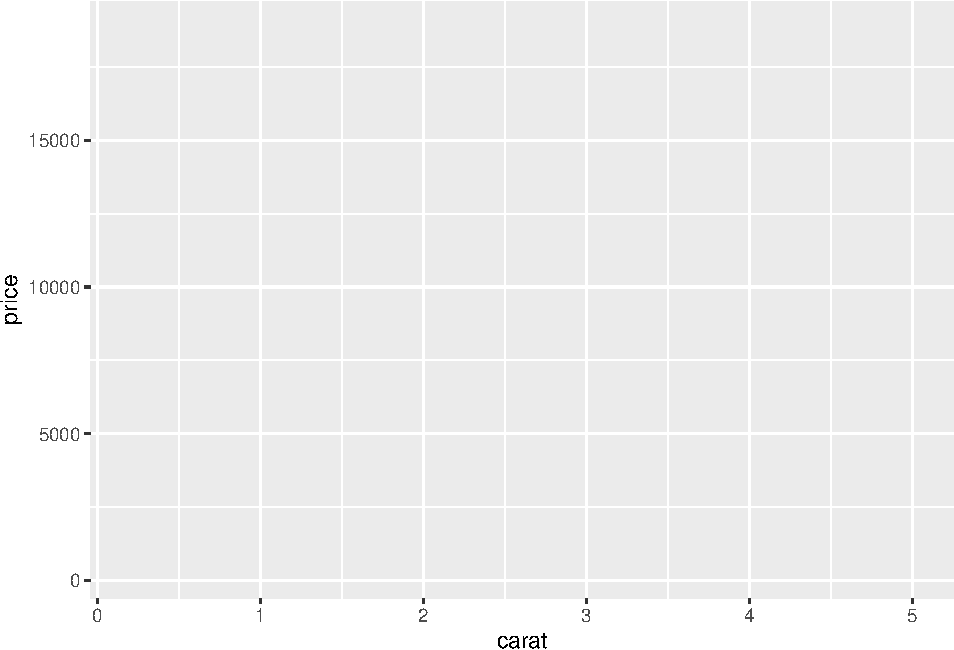
\includegraphics{Introduction-to-R,-Rstudio,-and-ggplot2_files/figure-latex/unnamed-chunk-4-1.pdf}

\begin{Shaded}
\begin{Highlighting}[]
\CommentTok{# geom_points() adds a new layer to a plot by drawing points to produce a scatter plot }
\KeywordTok{ggplot}\NormalTok{(}\DataTypeTok{data =}\NormalTok{ diamonds, }\KeywordTok{aes}\NormalTok{(}\DataTypeTok{x =}\NormalTok{ carat, }\DataTypeTok{y =}\NormalTok{ price)) }\OperatorTok{+}\StringTok{ }\KeywordTok{geom_point}\NormalTok{()}
\end{Highlighting}
\end{Shaded}

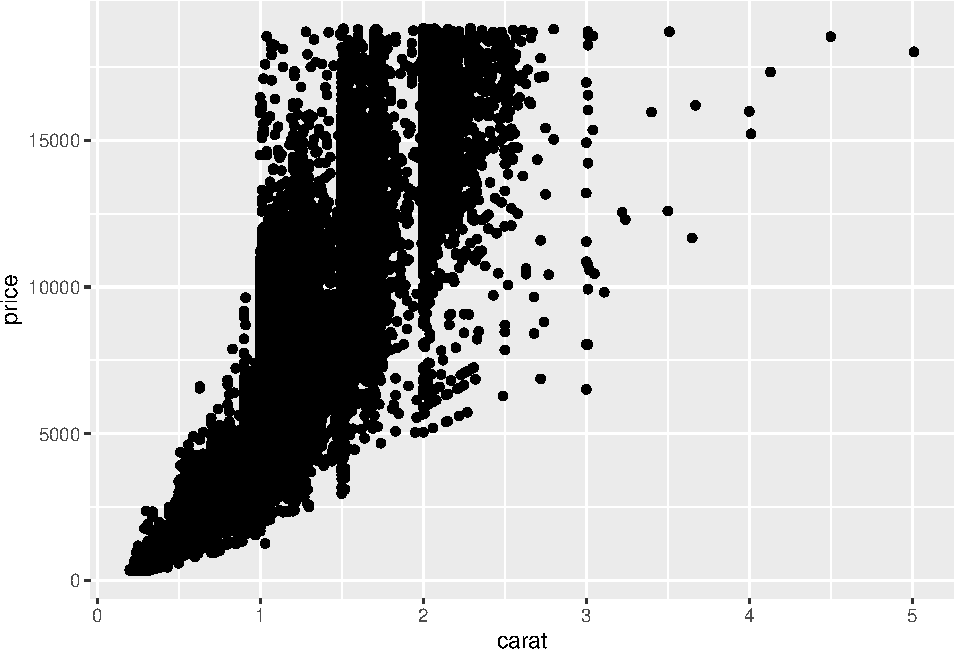
\includegraphics{Introduction-to-R,-Rstudio,-and-ggplot2_files/figure-latex/unnamed-chunk-5-1.pdf}

\begin{Shaded}
\begin{Highlighting}[]
\CommentTok{# geom_smooth() adds an additional layer to the plot by drawing a smoothed line to capture the trend in the scatterplot}
\KeywordTok{ggplot}\NormalTok{(}\DataTypeTok{data =}\NormalTok{ diamonds, }\KeywordTok{aes}\NormalTok{(}\DataTypeTok{x =}\NormalTok{ carat, }\DataTypeTok{y =}\NormalTok{ price)) }\OperatorTok{+}\StringTok{ }\KeywordTok{geom_point}\NormalTok{() }\OperatorTok{+}\StringTok{ }\KeywordTok{geom_smooth}\NormalTok{()}
\end{Highlighting}
\end{Shaded}

\begin{verbatim}
## `geom_smooth()` using method = 'gam' and formula 'y ~ s(x, bs = "cs")'
\end{verbatim}

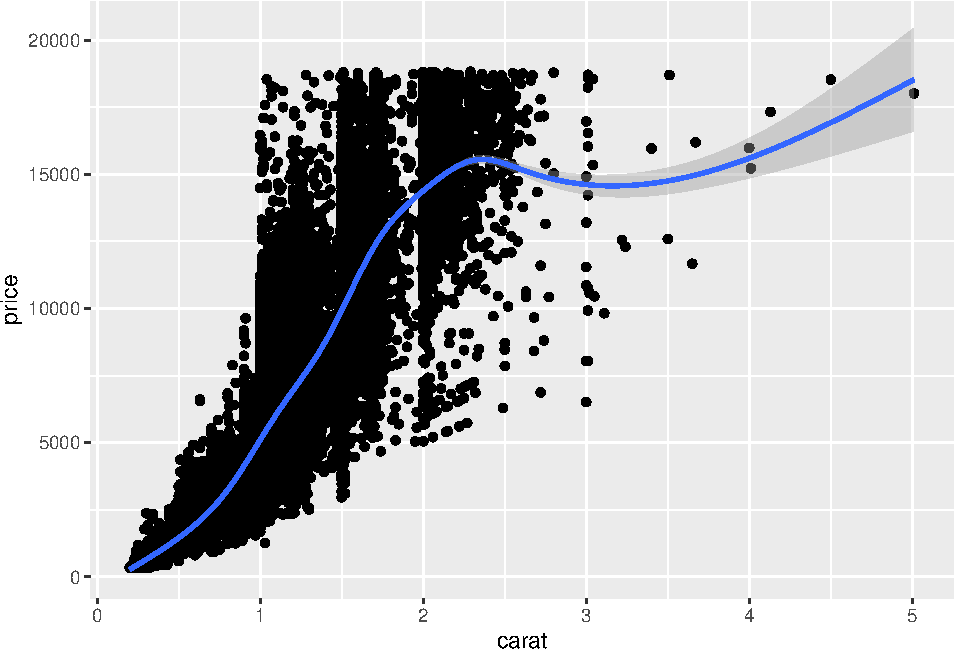
\includegraphics{Introduction-to-R,-Rstudio,-and-ggplot2_files/figure-latex/unnamed-chunk-6-1.pdf}

\textbf{Exercise}

\begin{itemize}
\item
  Create code chunks (gray area in a rmd file) using a short cut key (Mac: Command + Option + I; Windows: Ctrl + Alt + I).
\item
  Typing \texttt{mtcars} in your code chunks will display the content of the \texttt{mtcars} dataset. How can we display the help document for the \texttt{mtcars} data?
\item
  Type \texttt{head(mtcars)}. What did \texttt{head()} do? Check the help document of \texttt{head()} (\texttt{mtcar} is a dataframe in base R, whereas the \texttt{diamonds} is a tibble in \texttt{tidyverse}).
\item
  Using the \texttt{mtcars} data, plot the scatter plot between \texttt{mpg} (miles per gallon: y axis) and \texttt{disp} (displacement: x axis) with a smoothed line.
\end{itemize}

\hypertarget{aesthetic-mappings}{%
\subsection{Aesthetic mappings}\label{aesthetic-mappings}}

\begin{itemize}
\item
  ``A set of aesthetic mappings describe how \textbf{variables in the data} are mapped to \textbf{aesthetic properties} of the layer'' \citep{ggplot2}
\item
  ``To describe the way that \textbf{variables in the data} are mapped to \textbf{things that we can perceive on the plot (the "aesthetics")}, we use the \texttt{aes} function. The \texttt{aes} function takes a list of \textbf{aesthetic-variable pairs} like these: \texttt{aes(x\ =\ weight,\ y\ =\ height,\ colour\ =\ age)}. Here we are mapping x-position to \texttt{weight}, y-position to \texttt{height} and colour to \texttt{age}. The first two arguments can be left without names, in which case they correspond to the x and y variables.'' \citep{ggplot2}
\item
  Aesthetic properties include

  \begin{itemize}
  \tightlist
  \item
    \texttt{position} (e.g., x and y coordinates)
  \item
    \texttt{color} (outside color)
  \item
    \texttt{fill} (inside color)
  \item
    \texttt{shape} (of points; e.g., circle, triangle)
  \item
    \texttt{linetype} (e.g., solid line, dotted line)
  \item
    \texttt{size}
  \item
    \texttt{alpha} (transparency)
  \end{itemize}
\end{itemize}

\begin{Shaded}
\begin{Highlighting}[]
\CommentTok{# `color = color` maps the variable `color` in the dataset to the `color` aesthetics of points to encode further information in the graphic. }
\KeywordTok{ggplot}\NormalTok{(}\DataTypeTok{data =}\NormalTok{ diamonds, }\KeywordTok{aes}\NormalTok{(}\DataTypeTok{x =}\NormalTok{ carat, }\DataTypeTok{y =}\NormalTok{ price, }\DataTypeTok{color =}\NormalTok{ color)) }\OperatorTok{+}\StringTok{ }\KeywordTok{geom_point}\NormalTok{()}
\end{Highlighting}
\end{Shaded}

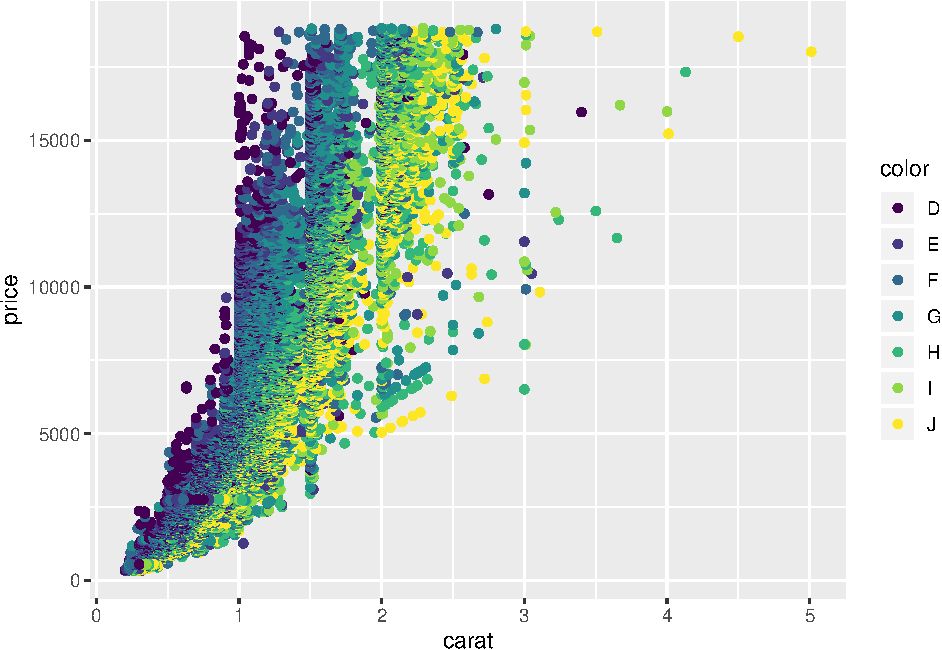
\includegraphics{Introduction-to-R,-Rstudio,-and-ggplot2_files/figure-latex/unnamed-chunk-7-1.pdf}

\begin{Shaded}
\begin{Highlighting}[]
\CommentTok{# `shape = cut` maps the `shape` aesthetics of points to the variable `cut` in the dataset to encode further information in the graphic. }
\CommentTok{# Note that the graphic is not so informative because points are overplotted. Sometimes, facetting may handle overplotting.  }
\KeywordTok{ggplot}\NormalTok{(}\DataTypeTok{data =}\NormalTok{ diamonds, }\KeywordTok{aes}\NormalTok{(}\DataTypeTok{x =}\NormalTok{ carat, }\DataTypeTok{y =}\NormalTok{ price, }\DataTypeTok{shape =}\NormalTok{ cut)) }\OperatorTok{+}\StringTok{ }\KeywordTok{geom_point}\NormalTok{()}
\end{Highlighting}
\end{Shaded}

\begin{verbatim}
## Warning: Using shapes for an ordinal variable is not advised
\end{verbatim}

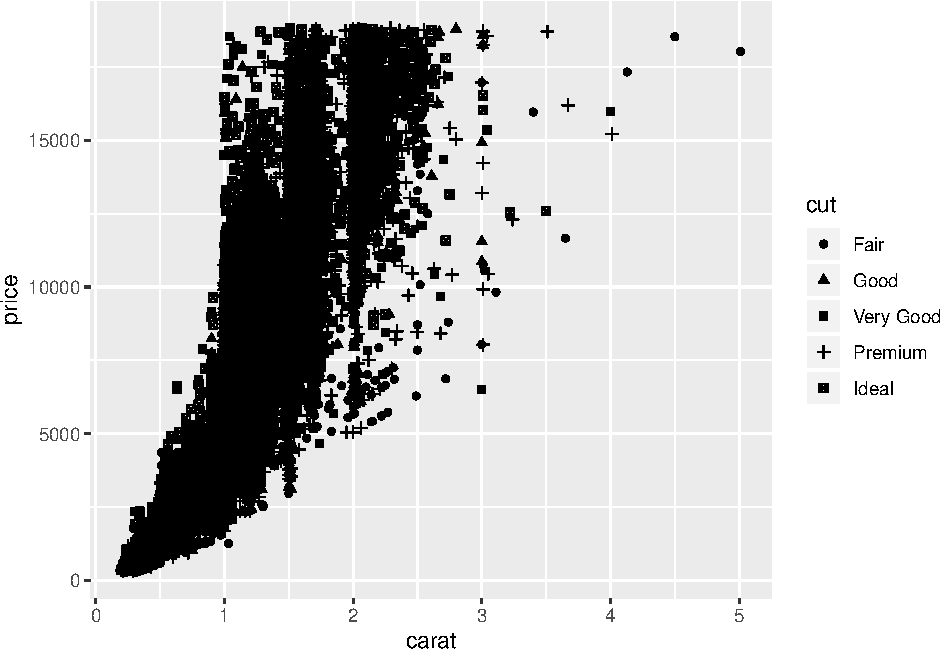
\includegraphics{Introduction-to-R,-Rstudio,-and-ggplot2_files/figure-latex/unnamed-chunk-8-1.pdf}

\begin{Shaded}
\begin{Highlighting}[]
\CommentTok{# We can set aesthetic properties to a constant outside aes() function. }
\KeywordTok{ggplot}\NormalTok{(}\DataTypeTok{data =}\NormalTok{ diamonds, }\KeywordTok{aes}\NormalTok{(}\DataTypeTok{x =}\NormalTok{ carat, }\DataTypeTok{y =}\NormalTok{ price)) }\OperatorTok{+}\StringTok{ }\KeywordTok{geom_point}\NormalTok{(}\DataTypeTok{color =} \StringTok{"blue"}\NormalTok{)}
\end{Highlighting}
\end{Shaded}

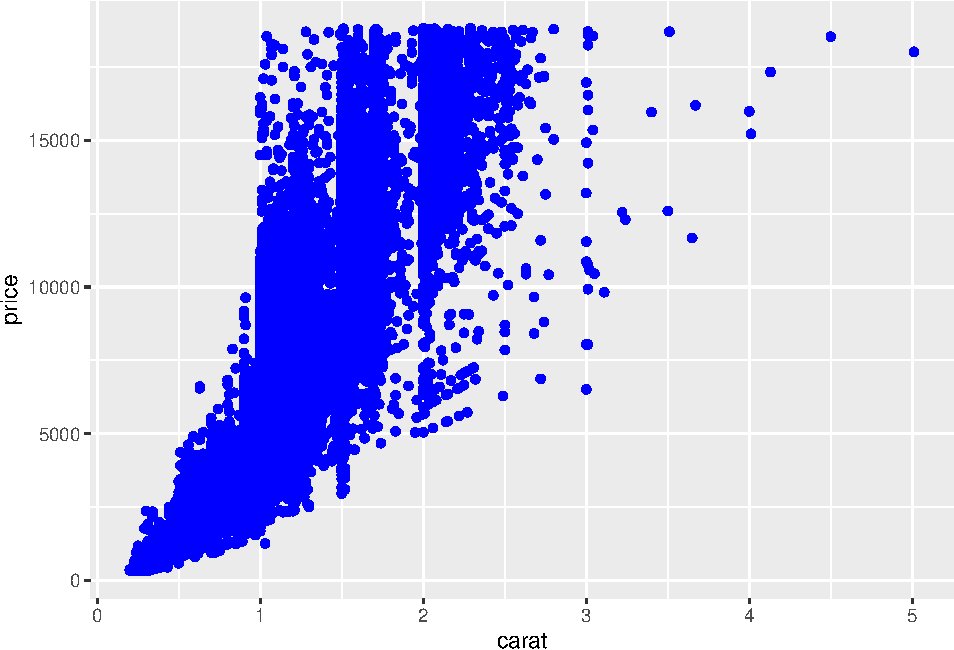
\includegraphics{Introduction-to-R,-Rstudio,-and-ggplot2_files/figure-latex/unnamed-chunk-9-1.pdf}

\textbf{Exercise}

\begin{itemize}
\item
  \texttt{mpg} is similar to \texttt{mtcars} but is a built-in tibble in \texttt{ggplot2}. 1) Plot \texttt{hwy} (mile per gallon: y axis) against \texttt{displ} (engine displancement: x axis), 2) Given the plot from 1), map the \texttt{class} variable to color, shape, alpha, and size aesthetics.
\item
  Explain what happens.
\end{itemize}

\begin{Shaded}
\begin{Highlighting}[]
\KeywordTok{ggplot}\NormalTok{(}\DataTypeTok{data =}\NormalTok{ mpg, }\DataTypeTok{mapping =} \KeywordTok{aes}\NormalTok{(}\DataTypeTok{x =}\NormalTok{ displ, }\DataTypeTok{y =}\NormalTok{ hwy, }\DataTypeTok{color=}\NormalTok{drv)) }\OperatorTok{+}\StringTok{ }\KeywordTok{geom_point}\NormalTok{() }\OperatorTok{+}\StringTok{ }\KeywordTok{geom_smooth}\NormalTok{(}\DataTypeTok{method=}\StringTok{"lm"}\NormalTok{)}
\end{Highlighting}
\end{Shaded}

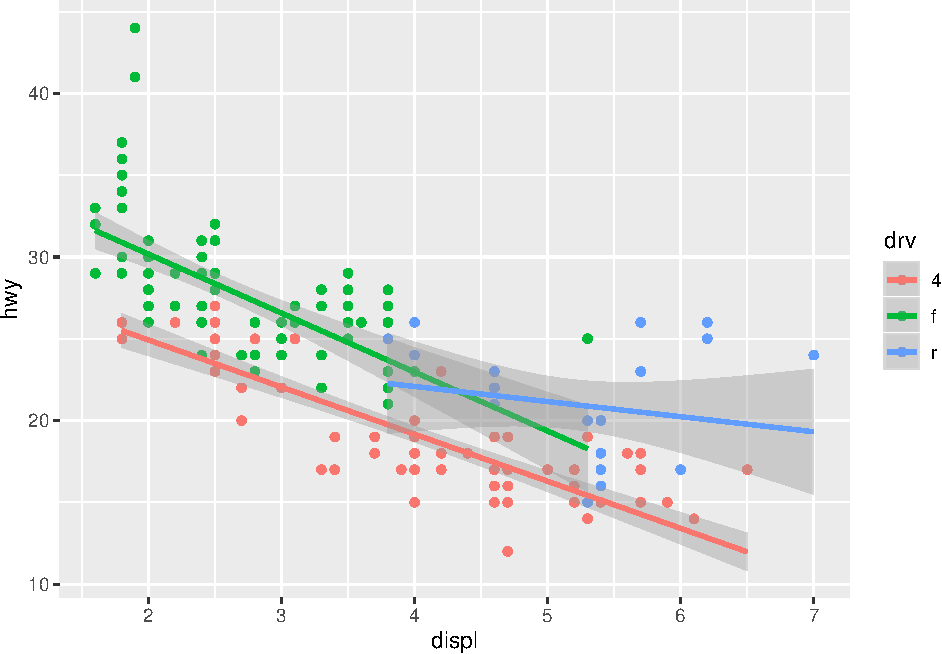
\includegraphics{Introduction-to-R,-Rstudio,-and-ggplot2_files/figure-latex/unnamed-chunk-10-1.pdf}

\begin{itemize}
\tightlist
\item
  This is what happens when mapping \texttt{x}, \texttt{y}, and \texttt{color} aesthetics to \texttt{hyw}, \texttt{displ}, and \texttt{cyl} variables: R creates a new dataset that contains all the data to be displayed on the plot.
\end{itemize}

\begin{longtable}[]{@{}lll@{}}
\toprule
x & y & color\tabularnewline
\midrule
\endhead
1.8 & 29 & 4\tabularnewline
1.8 & 29 & 4\tabularnewline
2.0 & 31 & 4\tabularnewline
2.0 & 30 & 4\tabularnewline
2.8 & 26 & 6\tabularnewline
2.8 & 26 & 6\tabularnewline
3.1 & 27 & 6\tabularnewline
1.8 & 26 & 4\tabularnewline
1.8 & 25 & 4\tabularnewline
2.0 & 28 & 4\tabularnewline
\bottomrule
\end{longtable}

\hypertarget{scales}{%
\subsection{Scales}\label{scales}}

\begin{itemize}
\item
  ``The scales map values in the data space to values in an aesthetic space, whether it be colour, or size, or shape. Scales draw a legend or axes, which provide an inverse mapping to make it possible to read the original data values from the graph.'' \citep{ggplot2}
\item
  In the previous table, computers don't know how to display colors based on 4, 6, \ldots{} Computers need a hexadecimal code for colors such as \texttt{FF6C91}. The mapping from the data to the final values that computers can use to display aesthetics is called \textbf{a scale}. In this sense, \textbf{a scale controls aesthetic mapping} from data to aesthetics. To control the mapping, use a custom scale using \texttt{scale\_*()} functions.
\end{itemize}

\begin{longtable}[]{@{}lll@{}}
\toprule
x & y & color\tabularnewline
\midrule
\endhead
1.8 & 29 & \#FF6C91\tabularnewline
1.8 & 29 & \#FF6C91\tabularnewline
2.0 & 31 & \#FF6C91\tabularnewline
2.0 & 30 & \#FF6C91\tabularnewline
2.8 & 26 & \#00C1A9\tabularnewline
2.8 & 26 & \#00C1A9\tabularnewline
3.1 & 27 & \#00C1A9\tabularnewline
1.8 & 26 & \#FF6C91\tabularnewline
1.8 & 25 & \#FF6C91\tabularnewline
2.0 & 28 & \#FF6C91\tabularnewline
\bottomrule
\end{longtable}

\begin{itemize}
\tightlist
\item
  e.g., \texttt{scale\_x\_continuous()} and \texttt{scale\_y\_continuous()} allow us to change the default scales for continuous \texttt{x} and \texttt{y} aesthetics: \url{https://ggplot2.tidyverse.org/reference/scale_continuous.html}.
\end{itemize}

\begin{Shaded}
\begin{Highlighting}[]
\NormalTok{p1 <-}\StringTok{ }\KeywordTok{ggplot}\NormalTok{(mpg, }\KeywordTok{aes}\NormalTok{(displ, hwy)) }\OperatorTok{+}\StringTok{ }\KeywordTok{geom_point}\NormalTok{()}
\NormalTok{p1}
\end{Highlighting}
\end{Shaded}

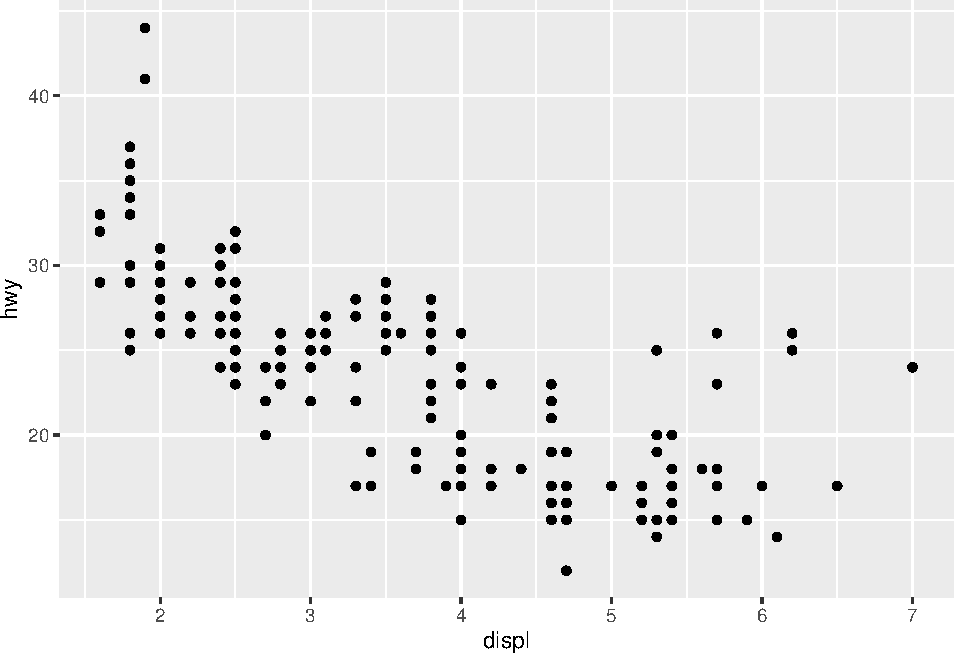
\includegraphics{Introduction-to-R,-Rstudio,-and-ggplot2_files/figure-latex/unnamed-chunk-11-1.pdf}

\begin{Shaded}
\begin{Highlighting}[]
\CommentTok{# change the axis labels}
\NormalTok{p1 }\OperatorTok{+}\StringTok{ }\KeywordTok{scale_x_continuous}\NormalTok{(}\StringTok{"Engine displacement (L)"}\NormalTok{) }\OperatorTok{+}
\StringTok{  }\KeywordTok{scale_y_continuous}\NormalTok{(}\StringTok{"Highway MPG"}\NormalTok{)}
\end{Highlighting}
\end{Shaded}

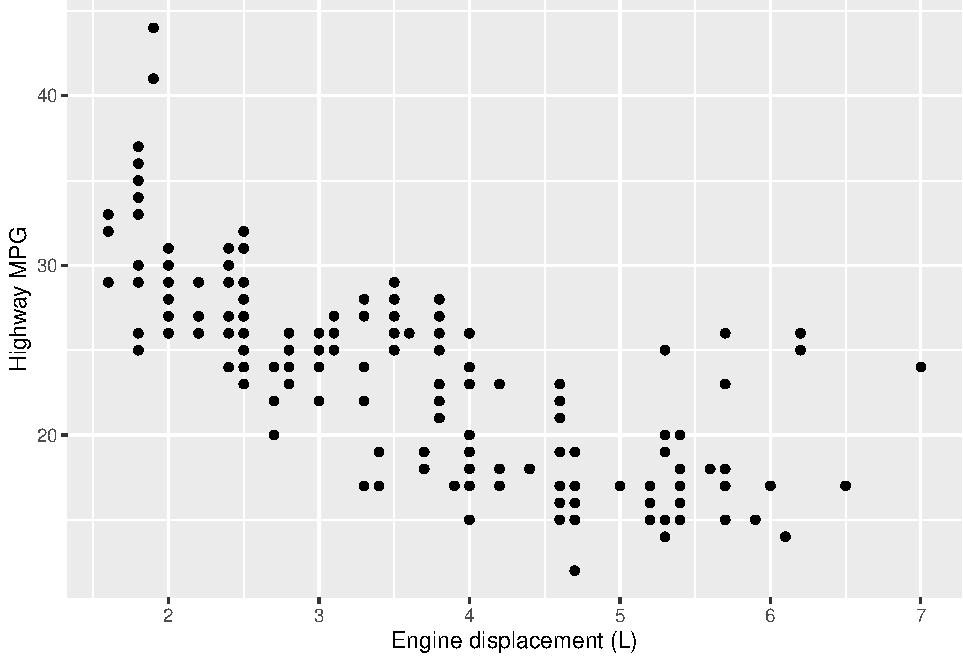
\includegraphics{Introduction-to-R,-Rstudio,-and-ggplot2_files/figure-latex/unnamed-chunk-12-1.pdf}

\begin{Shaded}
\begin{Highlighting}[]
\CommentTok{# also use the short-cut labs()}
\NormalTok{p1 }\OperatorTok{+}\StringTok{ }\KeywordTok{labs}\NormalTok{(}\DataTypeTok{x =} \StringTok{"Engine displacement (L)"}\NormalTok{, }\DataTypeTok{y =} \StringTok{"Highway MPG"}\NormalTok{)}
\end{Highlighting}
\end{Shaded}

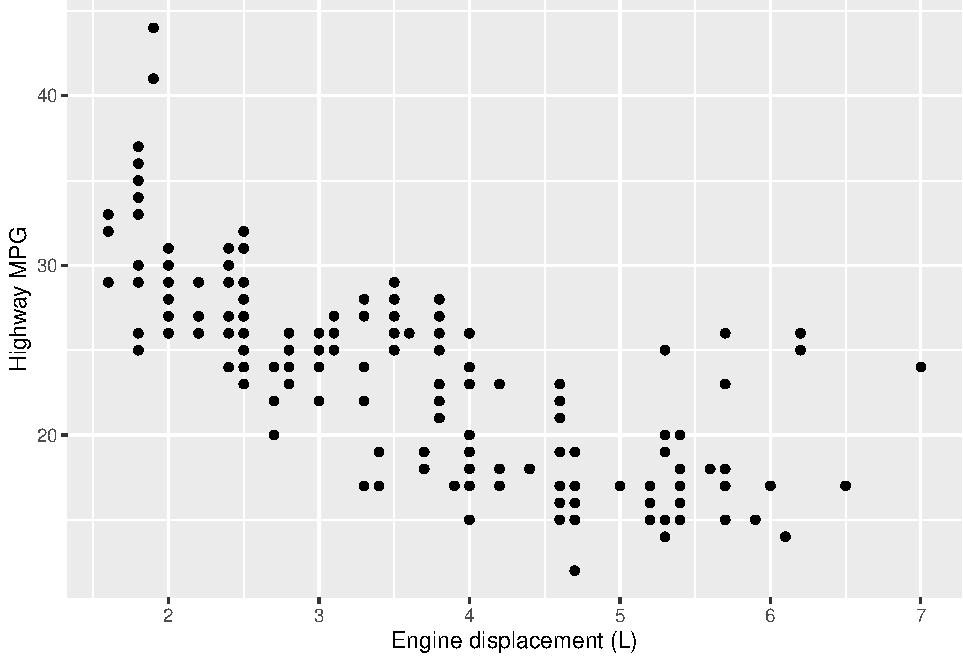
\includegraphics{Introduction-to-R,-Rstudio,-and-ggplot2_files/figure-latex/unnamed-chunk-13-1.pdf}

\begin{Shaded}
\begin{Highlighting}[]
\CommentTok{# modify the axis limits}
\NormalTok{p1 }\OperatorTok{+}\StringTok{ }\KeywordTok{scale_x_continuous}\NormalTok{(}\DataTypeTok{limits =} \KeywordTok{c}\NormalTok{(}\DecValTok{2}\NormalTok{, }\DecValTok{6}\NormalTok{))}
\end{Highlighting}
\end{Shaded}

\begin{verbatim}
## Warning: Removed 27 rows containing missing values (geom_point).
\end{verbatim}

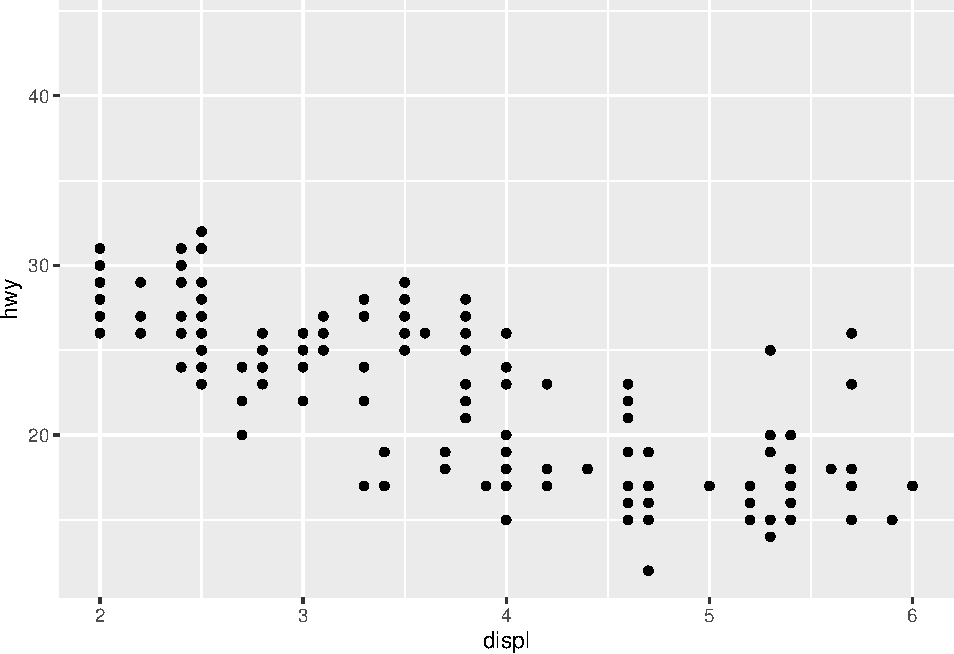
\includegraphics{Introduction-to-R,-Rstudio,-and-ggplot2_files/figure-latex/unnamed-chunk-14-1.pdf}

\begin{Shaded}
\begin{Highlighting}[]
\CommentTok{# use the short hand functions `xlim()` and `ylim()`}
\NormalTok{p1 }\OperatorTok{+}\StringTok{ }\KeywordTok{xlim}\NormalTok{(}\DecValTok{2}\NormalTok{, }\DecValTok{6}\NormalTok{)}
\end{Highlighting}
\end{Shaded}

\begin{verbatim}
## Warning: Removed 27 rows containing missing values (geom_point).
\end{verbatim}

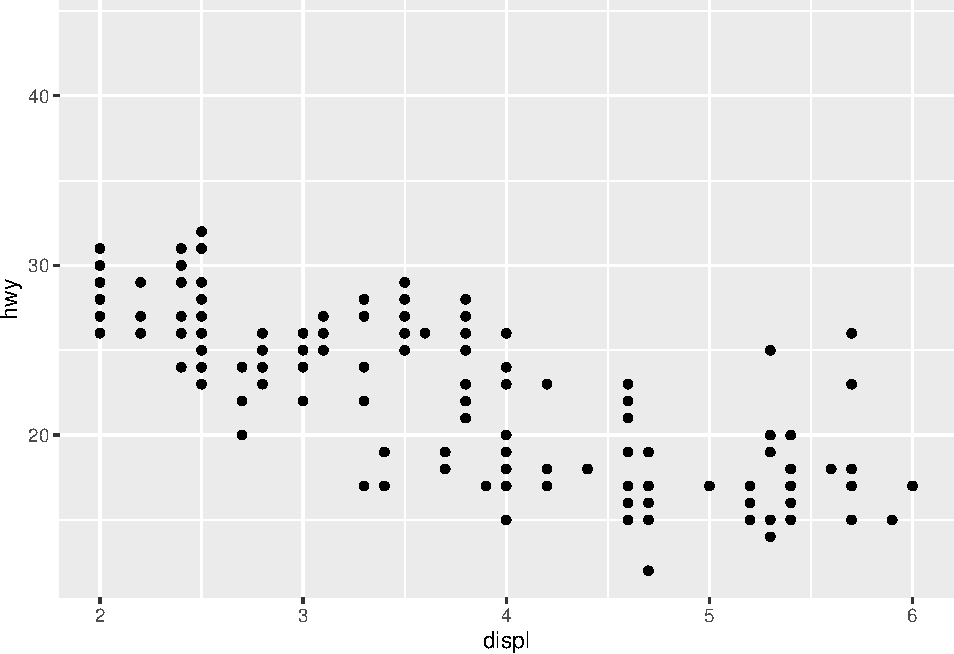
\includegraphics{Introduction-to-R,-Rstudio,-and-ggplot2_files/figure-latex/unnamed-chunk-15-1.pdf}

\begin{Shaded}
\begin{Highlighting}[]
\CommentTok{#  choose where the ticks appear}
\NormalTok{p1 }\OperatorTok{+}\StringTok{ }\KeywordTok{scale_x_continuous}\NormalTok{(}\DataTypeTok{breaks =} \KeywordTok{c}\NormalTok{(}\DecValTok{2}\NormalTok{, }\DecValTok{4}\NormalTok{, }\DecValTok{6}\NormalTok{))}
\end{Highlighting}
\end{Shaded}

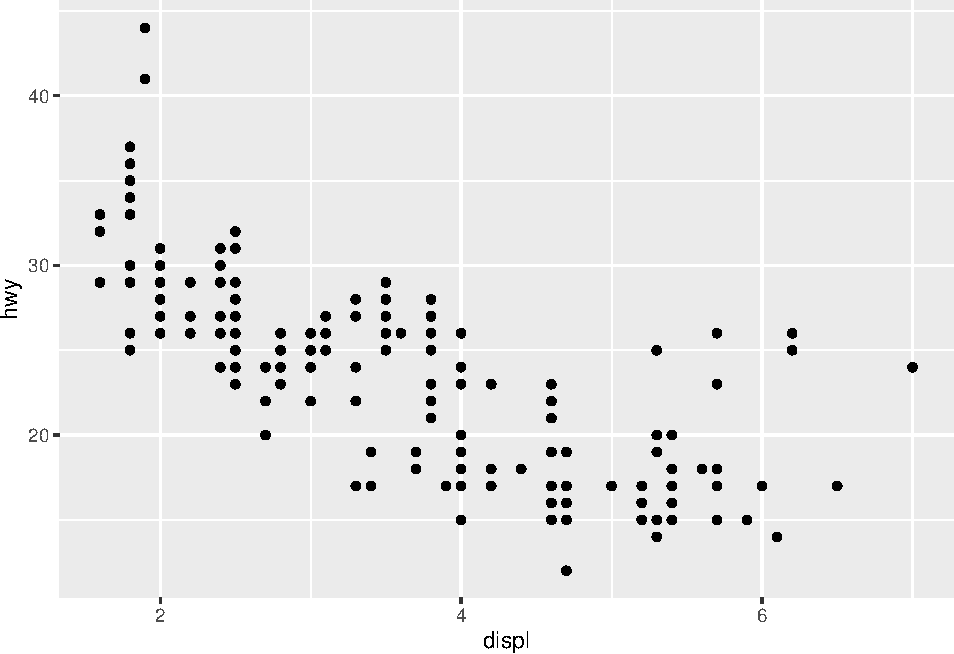
\includegraphics{Introduction-to-R,-Rstudio,-and-ggplot2_files/figure-latex/unnamed-chunk-16-1.pdf}

\begin{Shaded}
\begin{Highlighting}[]
\CommentTok{#  choose your own labels}
\NormalTok{p1 }\OperatorTok{+}\StringTok{ }\KeywordTok{scale_x_continuous}\NormalTok{(}\DataTypeTok{breaks =} \KeywordTok{c}\NormalTok{(}\DecValTok{2}\NormalTok{, }\DecValTok{4}\NormalTok{, }\DecValTok{6}\NormalTok{), }\DataTypeTok{label =} \KeywordTok{c}\NormalTok{(}\StringTok{"two"}\NormalTok{, }\StringTok{"four"}\NormalTok{, }\StringTok{"six"}\NormalTok{))}
\end{Highlighting}
\end{Shaded}

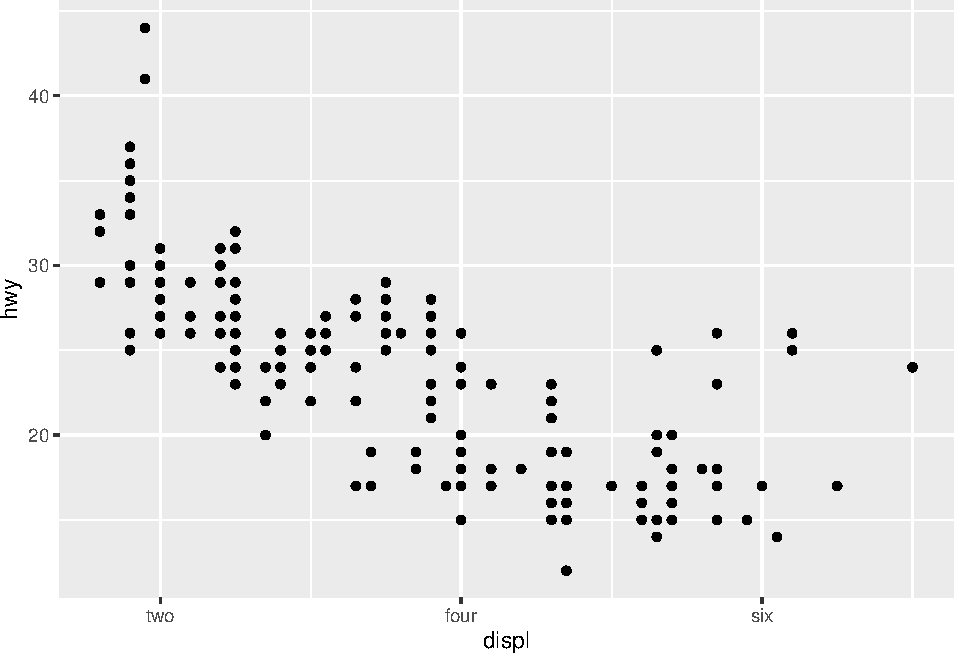
\includegraphics{Introduction-to-R,-Rstudio,-and-ggplot2_files/figure-latex/unnamed-chunk-17-1.pdf}

\begin{Shaded}
\begin{Highlighting}[]
\KeywordTok{ggplot}\NormalTok{(}\DataTypeTok{data =}\NormalTok{ mpg, }\DataTypeTok{mapping =} \KeywordTok{aes}\NormalTok{(}\DataTypeTok{x =}\NormalTok{ displ, }\DataTypeTok{y =}\NormalTok{ hwy, }\DataTypeTok{color=}\NormalTok{drv)) }\OperatorTok{+}\StringTok{ }\KeywordTok{geom_point}\NormalTok{() }\OperatorTok{+}\StringTok{ }\KeywordTok{geom_smooth}\NormalTok{(}\DataTypeTok{method=}\StringTok{"lm"}\NormalTok{) }\OperatorTok{+}\StringTok{ }\KeywordTok{labs}\NormalTok{(}\DataTypeTok{title =}\StringTok{"MPG vs Engine size"}\NormalTok{, }\DataTypeTok{x =} \StringTok{"Engine size"}\NormalTok{, }\DataTypeTok{y =} \StringTok{"MPG"}\NormalTok{)}
\end{Highlighting}
\end{Shaded}

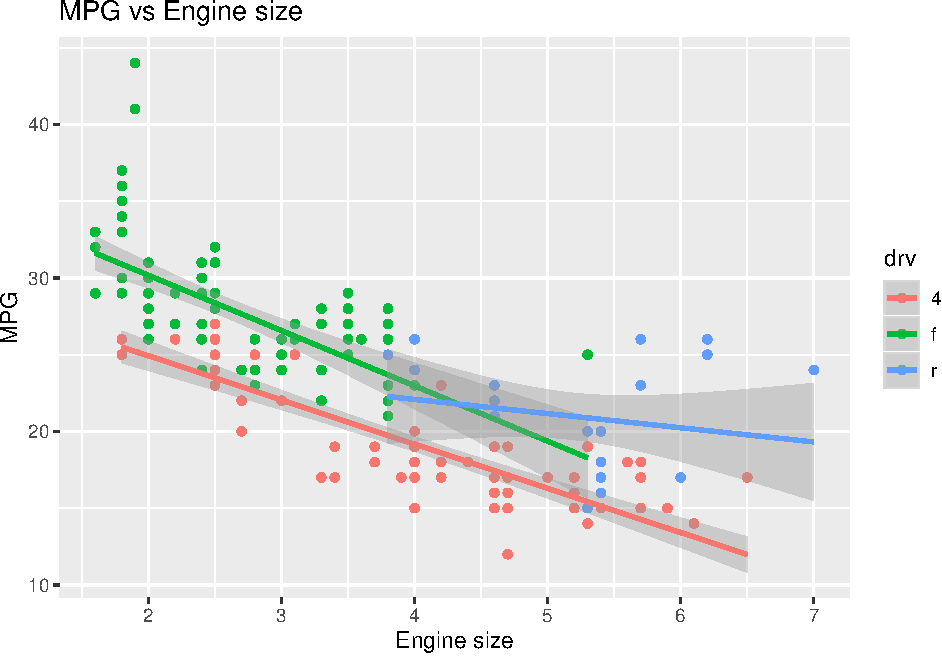
\includegraphics{Introduction-to-R,-Rstudio,-and-ggplot2_files/figure-latex/unnamed-chunk-18-1.pdf}

\begin{Shaded}
\begin{Highlighting}[]
\CommentTok{# Create your own discrete scale}
\KeywordTok{ggplot}\NormalTok{(}\DataTypeTok{data =}\NormalTok{ mpg, }\DataTypeTok{mapping =} \KeywordTok{aes}\NormalTok{(}\DataTypeTok{x =}\NormalTok{ displ, }\DataTypeTok{y =}\NormalTok{ hwy, }\DataTypeTok{color=}\NormalTok{drv)) }\OperatorTok{+}\StringTok{ }\KeywordTok{geom_point}\NormalTok{() }\OperatorTok{+}\StringTok{ }\KeywordTok{geom_smooth}\NormalTok{(}\DataTypeTok{method=}\StringTok{"lm"}\NormalTok{) }\OperatorTok{+}\StringTok{ }\KeywordTok{labs}\NormalTok{(}\DataTypeTok{title =}\StringTok{"MPG vs Engine size"}\NormalTok{, }\DataTypeTok{x =} \StringTok{"Engine size"}\NormalTok{, }\DataTypeTok{y =} \StringTok{"MPG"}\NormalTok{) }\OperatorTok{+}\StringTok{ }\KeywordTok{scale_colour_manual}\NormalTok{(}\DataTypeTok{name =} \StringTok{"Drive"}\NormalTok{, }\DataTypeTok{values =} \KeywordTok{c}\NormalTok{(}\StringTok{"lightpink"}\NormalTok{, }\StringTok{"darkseagreen"}\NormalTok{, }\StringTok{"lightblue"}\NormalTok{))}
\end{Highlighting}
\end{Shaded}

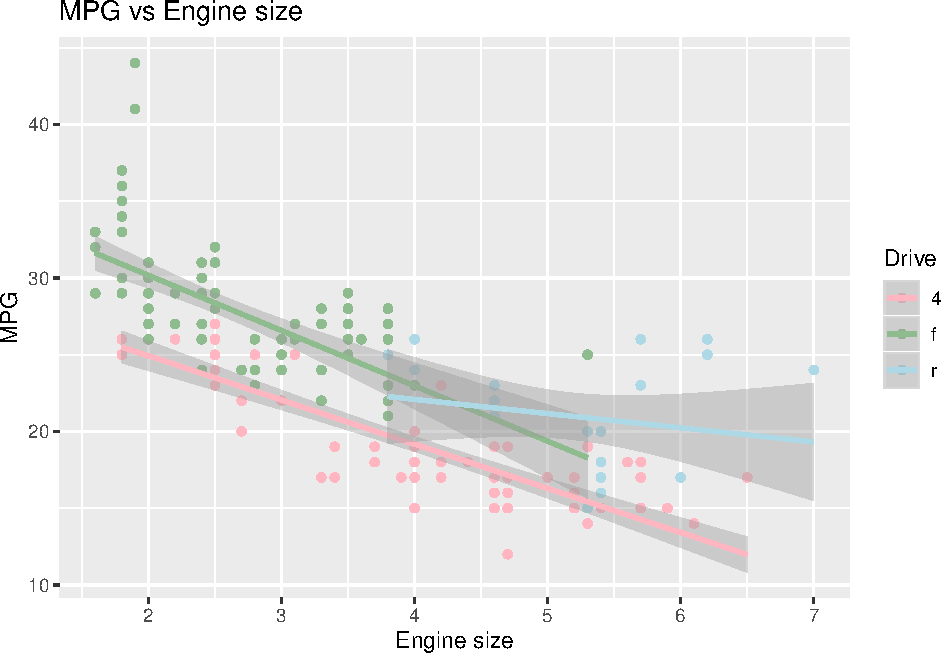
\includegraphics{Introduction-to-R,-Rstudio,-and-ggplot2_files/figure-latex/unnamed-chunk-19-1.pdf}

\begin{Shaded}
\begin{Highlighting}[]
\KeywordTok{ggplot}\NormalTok{(}\DataTypeTok{data =}\NormalTok{ mpg, }\DataTypeTok{mapping =} \KeywordTok{aes}\NormalTok{(}\DataTypeTok{x =}\NormalTok{ displ, }\DataTypeTok{y =}\NormalTok{ hwy, }\DataTypeTok{color=}\NormalTok{cty)) }\OperatorTok{+}\StringTok{ }\KeywordTok{geom_point}\NormalTok{() }
\end{Highlighting}
\end{Shaded}

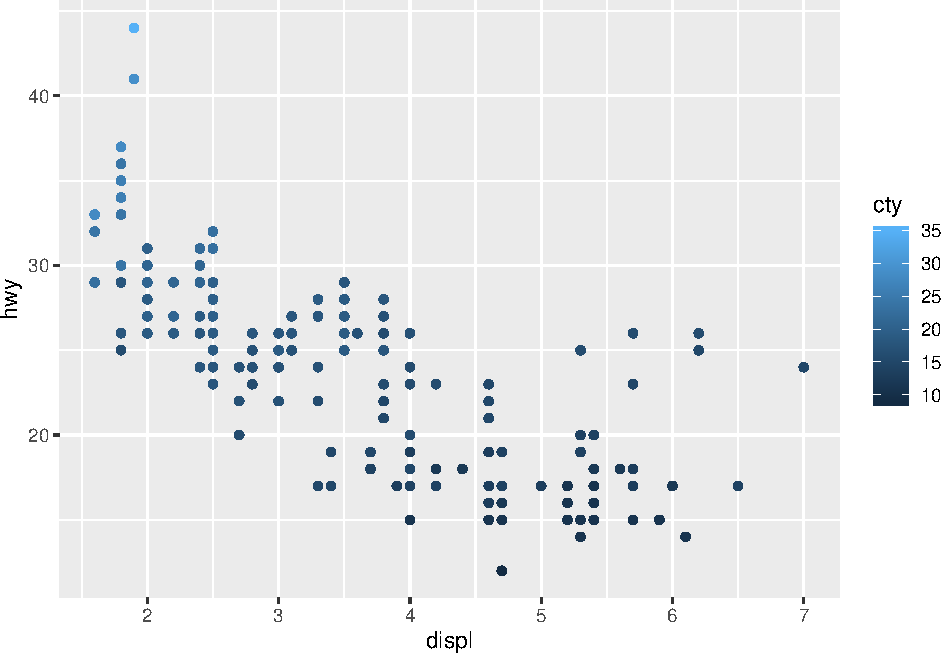
\includegraphics{Introduction-to-R,-Rstudio,-and-ggplot2_files/figure-latex/unnamed-chunk-20-1.pdf}

\begin{Shaded}
\begin{Highlighting}[]
\KeywordTok{ggplot}\NormalTok{(}\DataTypeTok{data =}\NormalTok{ mpg, }\DataTypeTok{mapping =} \KeywordTok{aes}\NormalTok{(}\DataTypeTok{x =}\NormalTok{ displ, }\DataTypeTok{y =}\NormalTok{ hwy, }\DataTypeTok{color=}\NormalTok{cty)) }\OperatorTok{+}\StringTok{ }\KeywordTok{geom_point}\NormalTok{() }\OperatorTok{+}\StringTok{ }\KeywordTok{scale_colour_gradient}\NormalTok{(}\DataTypeTok{name =} \StringTok{"City MPG"}\NormalTok{, }\DataTypeTok{low =} \StringTok{"red"}\NormalTok{, }\DataTypeTok{high =} \StringTok{"blue"}\NormalTok{)}
\end{Highlighting}
\end{Shaded}

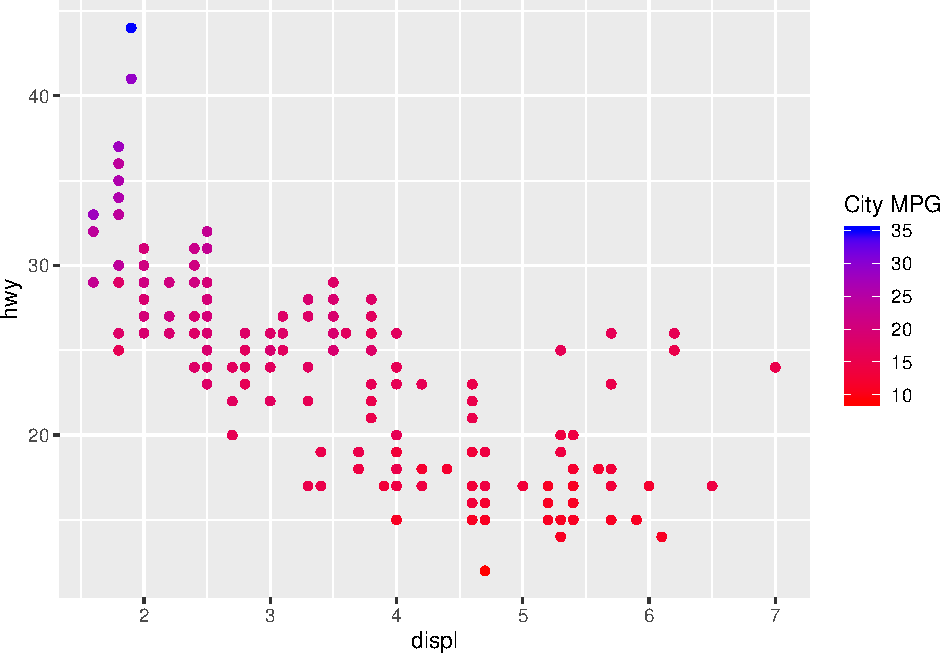
\includegraphics{Introduction-to-R,-Rstudio,-and-ggplot2_files/figure-latex/unnamed-chunk-21-1.pdf}

\begin{itemize}
\item
  For more details about scales, see \url{https://ggplot2.tidyverse.org/reference/}.
\item
  Colors in R: \url{http://www.sthda.com/english/wiki/colors-in-r}
\end{itemize}

\hypertarget{statistical-transformations-stats-for-short}{%
\subsection{\texorpdfstring{Statistical transformations (\textbf{stats} for short)}{Statistical transformations (stats for short)}}\label{statistical-transformations-stats-for-short}}

\begin{Shaded}
\begin{Highlighting}[]
\CommentTok{# historam shows the distribution of a single variable. }
\CommentTok{# where does the `count` in the plot come from? }
\KeywordTok{ggplot}\NormalTok{(}\DataTypeTok{data =}\NormalTok{ diamonds, }\KeywordTok{aes}\NormalTok{(}\DataTypeTok{x =}\NormalTok{ carat)) }\OperatorTok{+}\StringTok{ }\KeywordTok{geom_histogram}\NormalTok{()}
\end{Highlighting}
\end{Shaded}

\begin{verbatim}
## `stat_bin()` using `bins = 30`. Pick better value with `binwidth`.
\end{verbatim}

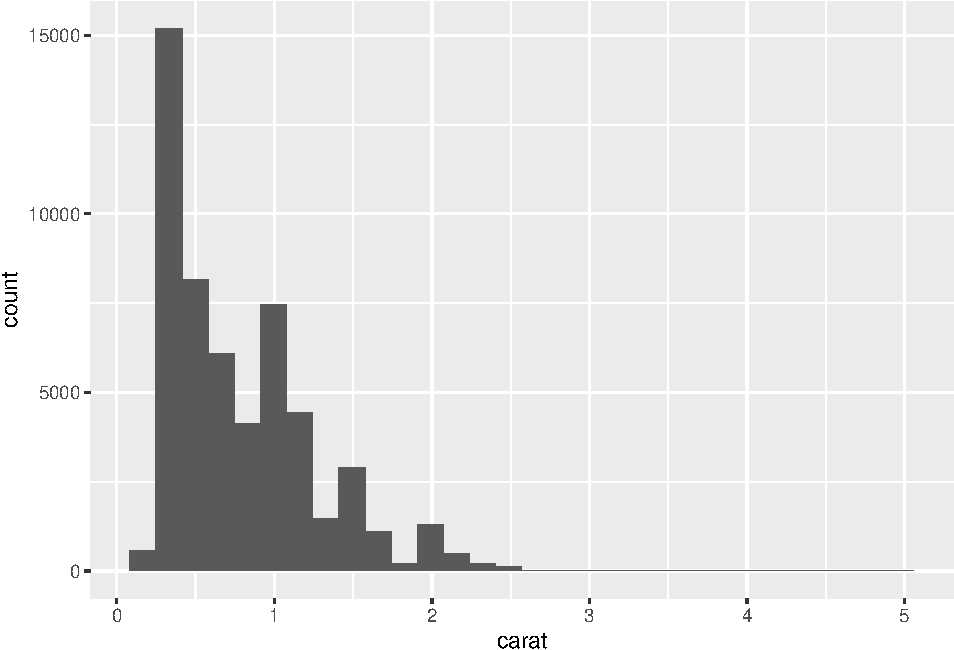
\includegraphics{Introduction-to-R,-Rstudio,-and-ggplot2_files/figure-latex/unnamed-chunk-22-1.pdf}

\begin{itemize}
\item
  ``Statistical transformations, \textbf{stats} for short, summarise data in many useful ways. For example, binning and counting observations to create a histogram, or summarising a 2d relationship with a linear model. Stats are optional, but very useful.'' \citep{ggplot2}
\item
  How \texttt{geom\_histogram()} works?

  \begin{itemize}
  \tightlist
  \item
    "A stat takes a dataset as input and returns a dataset as output, and so a stat can add new variables to the original dataset. It is possible to map aesthetics to these new variables. For example, \texttt{stat\_bin}, the statistic used to make histograms, produces the following variables:

    \begin{itemize}
    \tightlist
    \item
      \texttt{count}, the number of observations in each bin
    \item
      \texttt{density}, the density of observations in each bin (percentage of total / bar
      width)
    \item
      \texttt{x}, the centre of the bin" \citep{ggplot2}
    \end{itemize}
  \item
    ``These generated variables can be used instead of the variables present in
    the original dataset. For example, the default histogram geom assigns the height of the bars to the number of observations (\texttt{count}), but if you'd prefer a more traditional histogram, you can use the density (\texttt{density}). The following example shows a density histogram of carat from the diamonds dataset.'' \citep{ggplot2}
  \end{itemize}
\end{itemize}

\begin{Shaded}
\begin{Highlighting}[]
\CommentTok{# The names of generated variables must be surrounded with ..}
 \KeywordTok{ggplot}\NormalTok{(diamonds, }\KeywordTok{aes}\NormalTok{(carat)) }\OperatorTok{+}\StringTok{ }\KeywordTok{geom_histogram}\NormalTok{(}\KeywordTok{aes}\NormalTok{(}\DataTypeTok{y =}\NormalTok{ ..density..), }\DataTypeTok{binwidth =} \FloatTok{0.1}\NormalTok{)}
\end{Highlighting}
\end{Shaded}

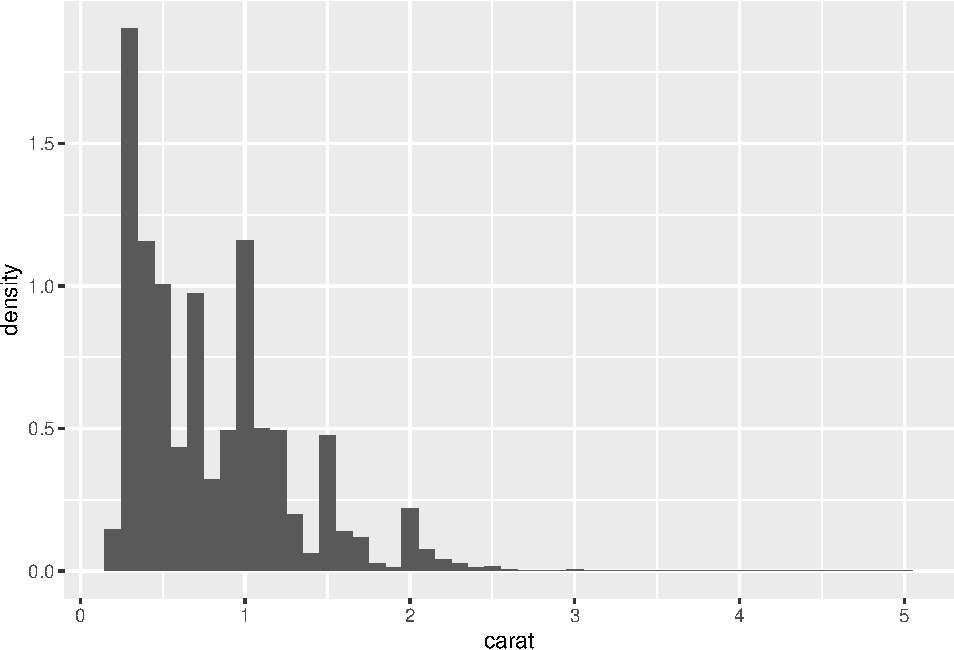
\includegraphics{Introduction-to-R,-Rstudio,-and-ggplot2_files/figure-latex/unnamed-chunk-23-1.pdf}

\begin{itemize}
\tightlist
\item
  Every \textbf{geom} has a default \textbf{stats}.
\end{itemize}

\begin{Shaded}
\begin{Highlighting}[]
\CommentTok{# An alternative way to build a layer}
 \KeywordTok{ggplot}\NormalTok{(diamonds, }\KeywordTok{aes}\NormalTok{(carat)) }\OperatorTok{+}\StringTok{ }\KeywordTok{stat_bin}\NormalTok{()}
\end{Highlighting}
\end{Shaded}

\begin{verbatim}
## `stat_bin()` using `bins = 30`. Pick better value with `binwidth`.
\end{verbatim}

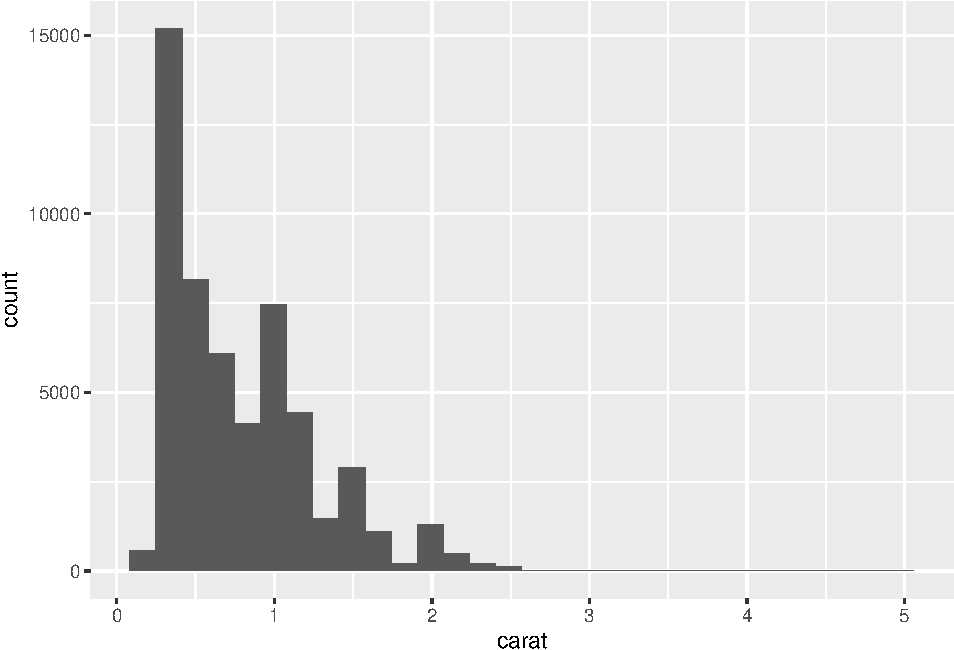
\includegraphics{Introduction-to-R,-Rstudio,-and-ggplot2_files/figure-latex/unnamed-chunk-24-1.pdf}

\begin{itemize}
\tightlist
\item
  Position adjustments

  \begin{itemize}
  \tightlist
  \item
    Position adjustments determine how to arrange \textbf{geoms} that would otherwise occupy the same space.
  \end{itemize}
\end{itemize}

\begin{Shaded}
\begin{Highlighting}[]
\CommentTok{# The discrete analogue of histogram is the bar plot}
\NormalTok{s <-}\StringTok{ }\KeywordTok{ggplot}\NormalTok{(mpg, }\KeywordTok{aes}\NormalTok{(fl, }\DataTypeTok{fill =}\NormalTok{ drv))}
\end{Highlighting}
\end{Shaded}

\begin{Shaded}
\begin{Highlighting}[]
\NormalTok{s }\OperatorTok{+}\StringTok{ }\KeywordTok{geom_bar}\NormalTok{()}
\end{Highlighting}
\end{Shaded}

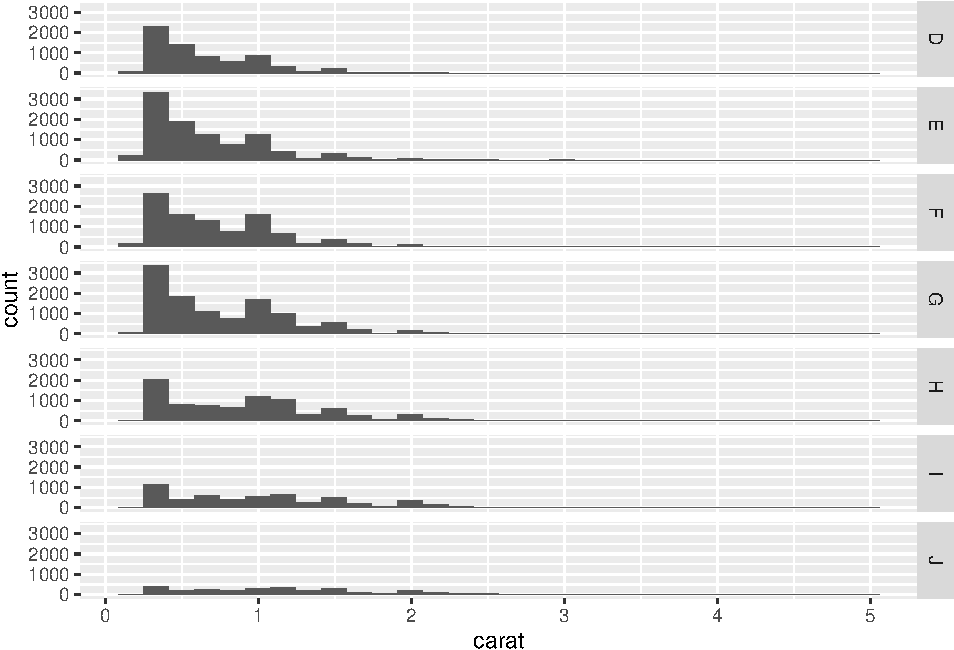
\includegraphics{Introduction-to-R,-Rstudio,-and-ggplot2_files/figure-latex/unnamed-chunk-26-1.pdf}

\begin{Shaded}
\begin{Highlighting}[]
\CommentTok{# Stack elements on top of one another}
\NormalTok{s }\OperatorTok{+}\StringTok{ }\KeywordTok{geom_bar}\NormalTok{(}\DataTypeTok{position =} \StringTok{"stack"}\NormalTok{)}
\end{Highlighting}
\end{Shaded}

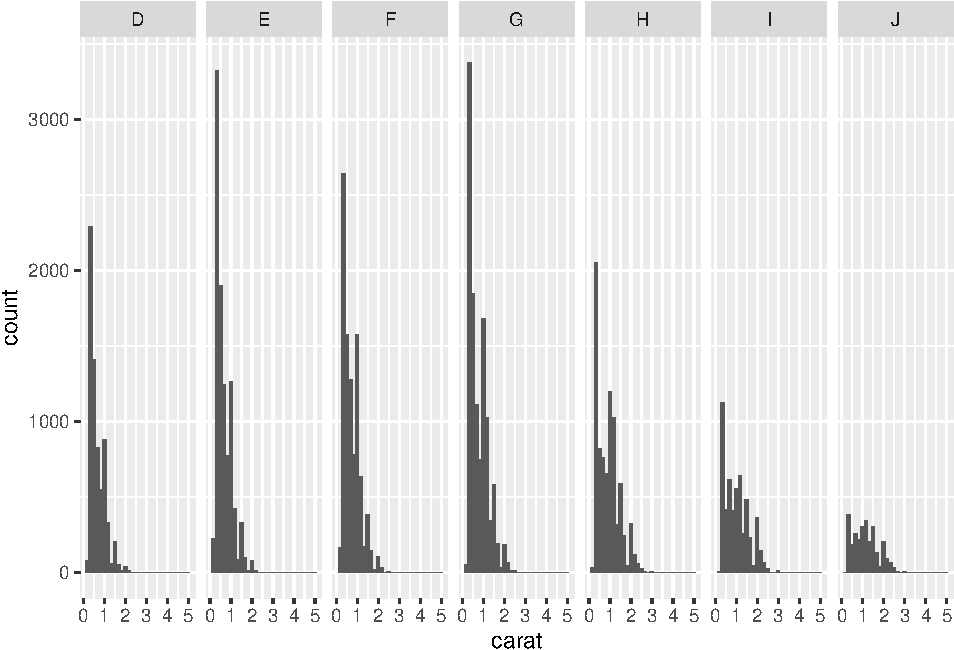
\includegraphics{Introduction-to-R,-Rstudio,-and-ggplot2_files/figure-latex/unnamed-chunk-27-1.pdf}

\begin{Shaded}
\begin{Highlighting}[]
\CommentTok{# Arrange elements side by side}
\NormalTok{s }\OperatorTok{+}\StringTok{ }\KeywordTok{geom_bar}\NormalTok{(}\DataTypeTok{position =} \StringTok{"dodge"}\NormalTok{)}
\end{Highlighting}
\end{Shaded}

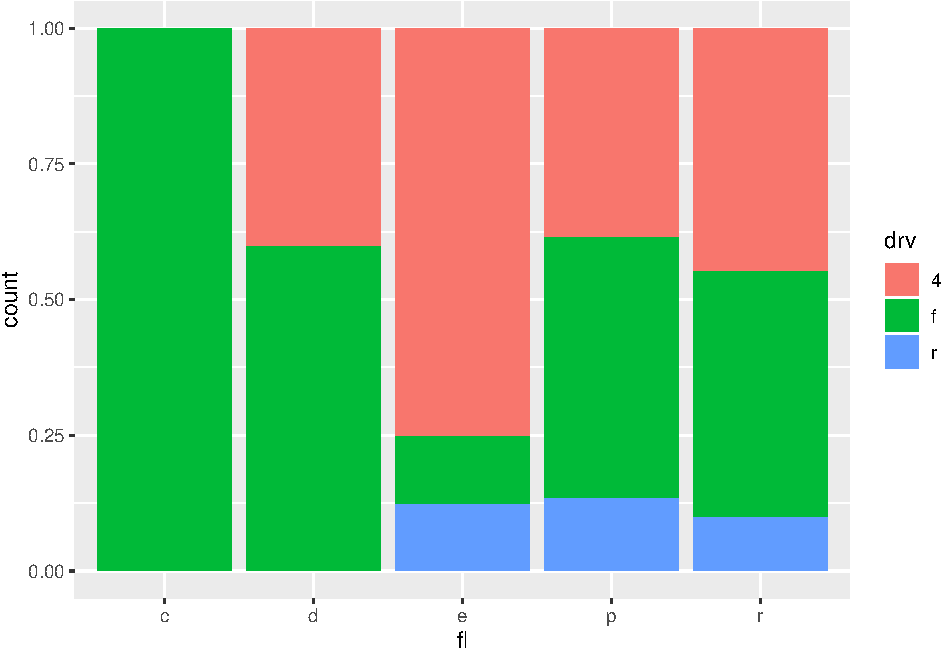
\includegraphics{Introduction-to-R,-Rstudio,-and-ggplot2_files/figure-latex/unnamed-chunk-28-1.pdf}

\begin{Shaded}
\begin{Highlighting}[]
\CommentTok{# Stack elements on top of one another,normalize height}
\NormalTok{s }\OperatorTok{+}\StringTok{ }\KeywordTok{geom_bar}\NormalTok{(}\DataTypeTok{position =} \StringTok{"fill"}\NormalTok{)}
\end{Highlighting}
\end{Shaded}

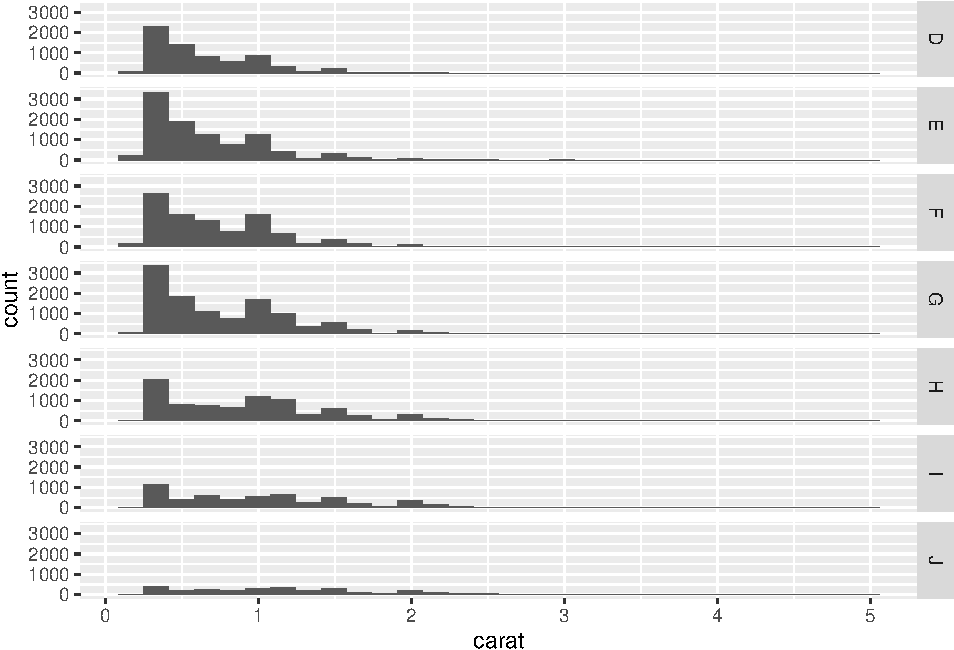
\includegraphics{Introduction-to-R,-Rstudio,-and-ggplot2_files/figure-latex/unnamed-chunk-29-1.pdf}

\hypertarget{a-faceting}{%
\subsection{A faceting}\label{a-faceting}}

\begin{itemize}
\item
  ``A faceting specification describes how to break up the data into \textbf{subsets} and how to display those subsets as \textbf{small multiples}. This is also known as \textbf{conditioning} or latticing/trellising.'' \citep{ggplot2}
\item
  ``There are two types of faceting provided by ggplot2: \texttt{facet\_grid} and \texttt{facet\_wrap}. Facet grid produces a 2d grid of panels defined by variables which form the rows and columns, while facet wrap produces a 1d ribbon of panels that is wrapped into 2d'' \citep{ggplot2}
\end{itemize}

\begin{Shaded}
\begin{Highlighting}[]
\CommentTok{# facet into rows}
\KeywordTok{ggplot}\NormalTok{(}\DataTypeTok{data =}\NormalTok{ diamonds, }\KeywordTok{aes}\NormalTok{(}\DataTypeTok{x =}\NormalTok{ carat)) }\OperatorTok{+}\StringTok{ }\KeywordTok{geom_histogram}\NormalTok{() }\OperatorTok{+}\StringTok{ }\KeywordTok{facet_grid}\NormalTok{(color }\OperatorTok{~}\StringTok{ }\NormalTok{.)}
\end{Highlighting}
\end{Shaded}

\begin{verbatim}
## `stat_bin()` using `bins = 30`. Pick better value with `binwidth`.
\end{verbatim}

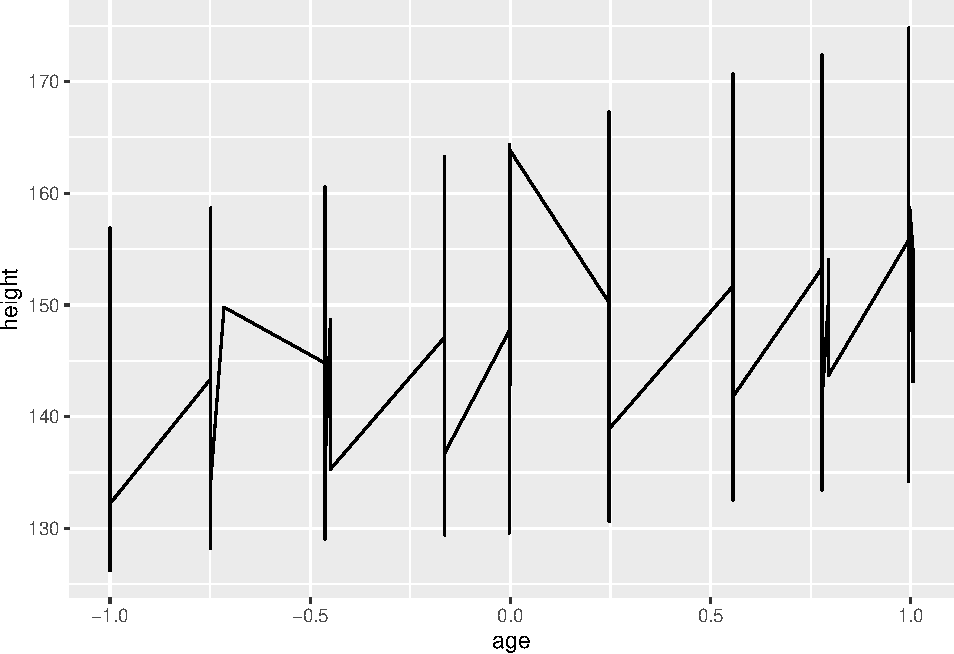
\includegraphics{Introduction-to-R,-Rstudio,-and-ggplot2_files/figure-latex/unnamed-chunk-30-1.pdf}

\begin{Shaded}
\begin{Highlighting}[]
\CommentTok{# facet into columns}
\KeywordTok{ggplot}\NormalTok{(}\DataTypeTok{data =}\NormalTok{ diamonds, }\KeywordTok{aes}\NormalTok{(}\DataTypeTok{x =}\NormalTok{ carat)) }\OperatorTok{+}\StringTok{ }\KeywordTok{geom_histogram}\NormalTok{() }\OperatorTok{+}\StringTok{ }\KeywordTok{facet_grid}\NormalTok{(. }\OperatorTok{~}\StringTok{ }\NormalTok{color)}
\end{Highlighting}
\end{Shaded}

\begin{verbatim}
## `stat_bin()` using `bins = 30`. Pick better value with `binwidth`.
\end{verbatim}

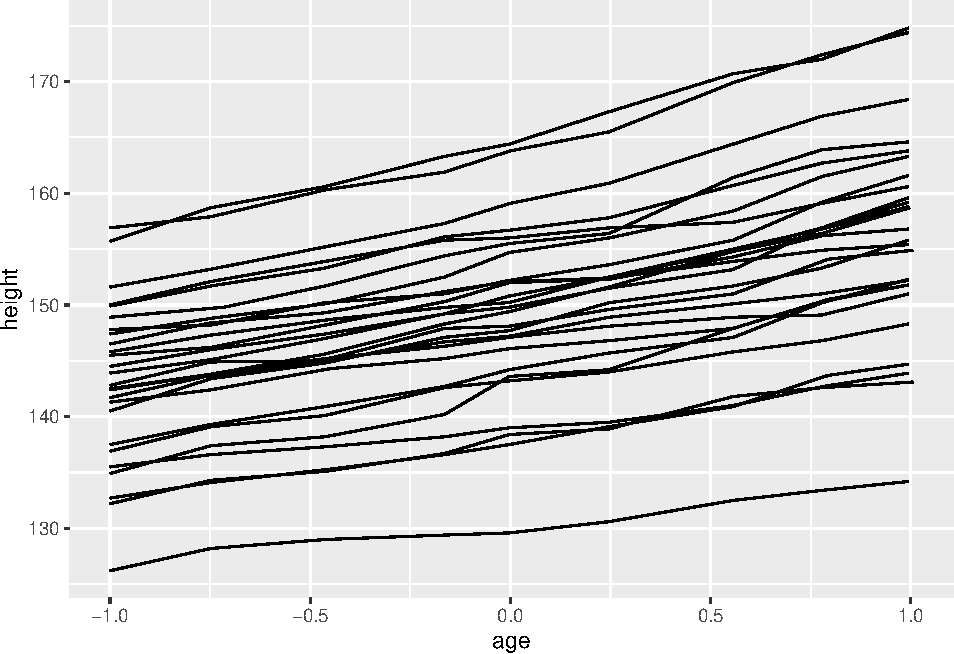
\includegraphics{Introduction-to-R,-Rstudio,-and-ggplot2_files/figure-latex/unnamed-chunk-31-1.pdf}

\textbf{Exercise}

\begin{itemize}
\item
  Using \texttt{mpg} data, plot \texttt{hwy} (y) vs \texttt{cty} (x).
\item
  facet into rows using \texttt{cyl}.
\item
  facet into columns using \texttt{cyl}.
\item
  facet into rows using \texttt{cyl} and columns using \texttt{year}
\end{itemize}

\hypertarget{grouping}{%
\subsection{Grouping}\label{grouping}}

\begin{itemize}
\item
  ``In many situations, you want to \textbf{separate your data into groups}, but render them in the same way. When looking at the data in aggregate you want to be able to distinguish individual subjects, but not identify them. This is common in \textbf{longitudinal studies} with many subjects, where the plots are often descriptively called spaghetti plots.'' \citep{ggplot2}
\item
  \texttt{Oxboys} is a dataset in the \texttt{nlme} package. \texttt{Oxboys} includes the height of a selection of boys from Oxford, England versus a standardized age.
\end{itemize}

\begin{Shaded}
\begin{Highlighting}[]
\KeywordTok{library}\NormalTok{(nlme)}
\end{Highlighting}
\end{Shaded}

\begin{Shaded}
\begin{Highlighting}[]
\CommentTok{# age = a numeric vector giving the standardized age }
\KeywordTok{head}\NormalTok{(Oxboys)}
\end{Highlighting}
\end{Shaded}

\begin{verbatim}
## Grouped Data: height ~ age | Subject
##   Subject     age height Occasion
## 1       1 -1.0000  140.5        1
## 2       1 -0.7479  143.4        2
## 3       1 -0.4630  144.8        3
## 4       1 -0.1643  147.1        4
## 5       1 -0.0027  147.7        5
## 6       1  0.2466  150.2        6
\end{verbatim}

\begin{Shaded}
\begin{Highlighting}[]
\KeywordTok{ggplot}\NormalTok{(Oxboys, }\KeywordTok{aes}\NormalTok{(age, height)) }\OperatorTok{+}\StringTok{ }\KeywordTok{geom_line}\NormalTok{()}
\end{Highlighting}
\end{Shaded}

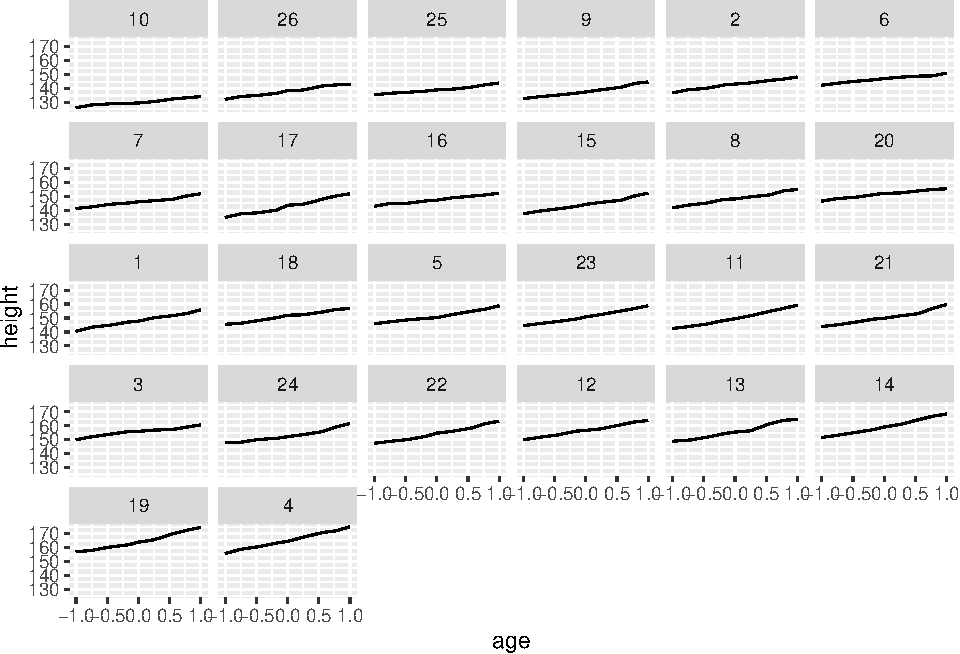
\includegraphics{Introduction-to-R,-Rstudio,-and-ggplot2_files/figure-latex/unnamed-chunk-34-1.pdf}

\begin{Shaded}
\begin{Highlighting}[]
\KeywordTok{ggplot}\NormalTok{(Oxboys, }\KeywordTok{aes}\NormalTok{(age, height, }\DataTypeTok{group =}\NormalTok{ Subject)) }\OperatorTok{+}\StringTok{ }\KeywordTok{geom_line}\NormalTok{()}
\end{Highlighting}
\end{Shaded}

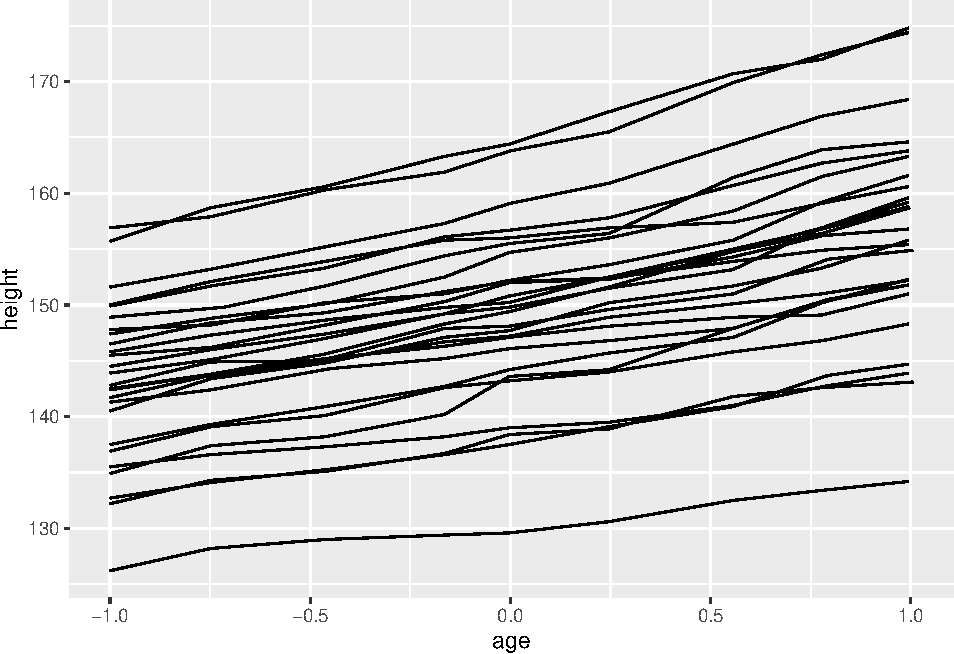
\includegraphics{Introduction-to-R,-Rstudio,-and-ggplot2_files/figure-latex/unnamed-chunk-35-1.pdf}

\begin{Shaded}
\begin{Highlighting}[]
\CommentTok{# In many cases, this is not what we want}
\KeywordTok{ggplot}\NormalTok{(Oxboys, }\KeywordTok{aes}\NormalTok{(age, height, }\DataTypeTok{group =}\NormalTok{ Subject)) }\OperatorTok{+}\StringTok{ }\KeywordTok{geom_line}\NormalTok{() }\OperatorTok{+}\StringTok{ }\KeywordTok{geom_smooth}\NormalTok{()}
\end{Highlighting}
\end{Shaded}

\begin{verbatim}
## `geom_smooth()` using method = 'loess' and formula 'y ~ x'
\end{verbatim}

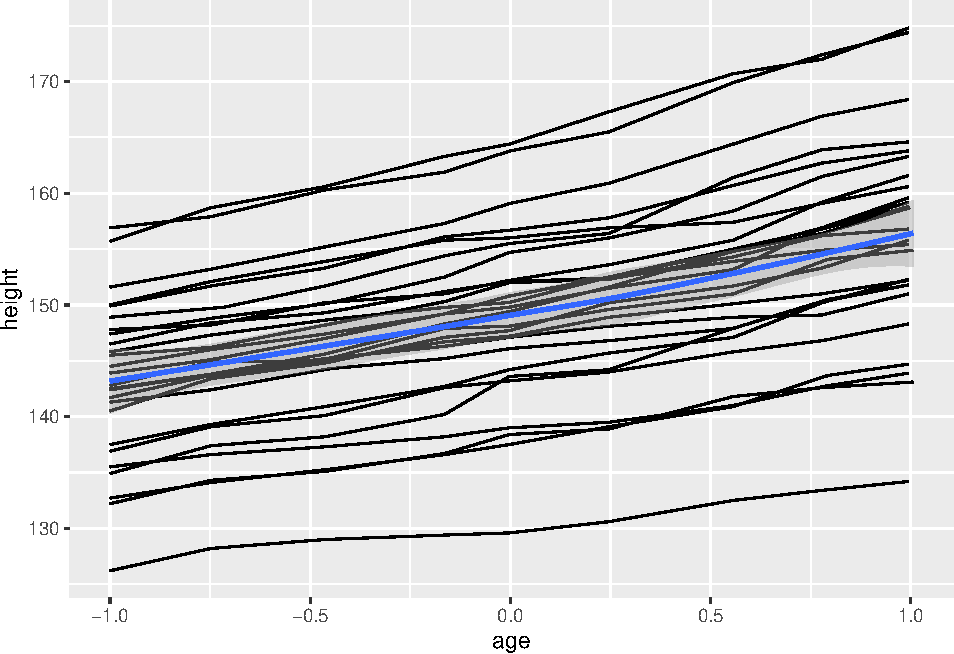
\includegraphics{Introduction-to-R,-Rstudio,-and-ggplot2_files/figure-latex/unnamed-chunk-36-1.pdf}

\begin{Shaded}
\begin{Highlighting}[]
\CommentTok{# group = 1 override the default grouping }
\KeywordTok{ggplot}\NormalTok{(Oxboys, }\KeywordTok{aes}\NormalTok{(age, height, }\DataTypeTok{group =}\NormalTok{ Subject)) }\OperatorTok{+}\StringTok{ }\KeywordTok{geom_line}\NormalTok{() }\OperatorTok{+}\StringTok{ }\KeywordTok{geom_smooth}\NormalTok{(}\KeywordTok{aes}\NormalTok{(}\DataTypeTok{group =} \DecValTok{1}\NormalTok{))}
\end{Highlighting}
\end{Shaded}

\begin{verbatim}
## `geom_smooth()` using method = 'loess' and formula 'y ~ x'
\end{verbatim}

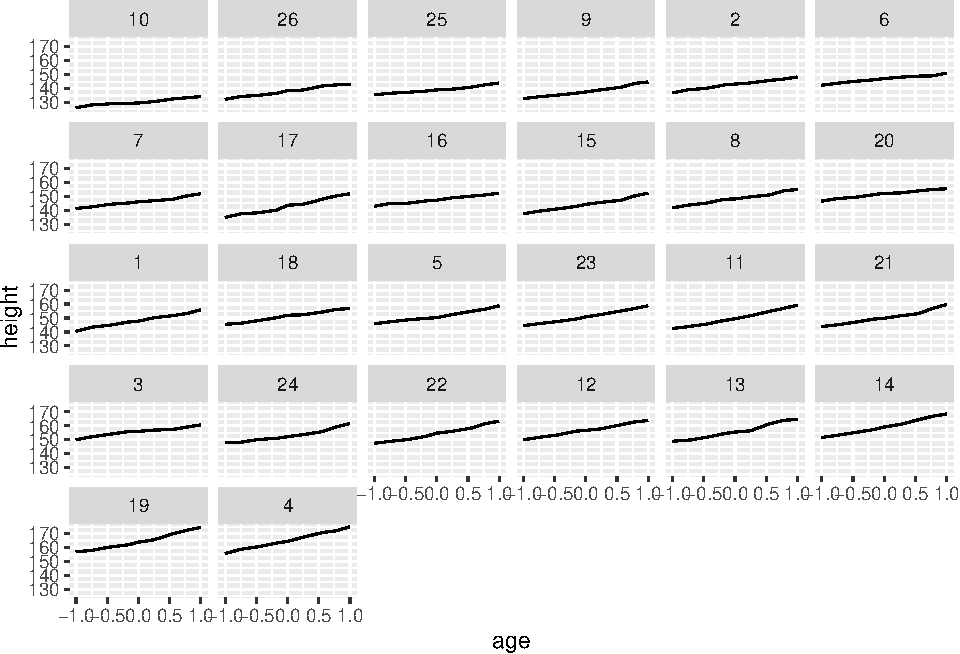
\includegraphics{Introduction-to-R,-Rstudio,-and-ggplot2_files/figure-latex/unnamed-chunk-37-1.pdf}

\begin{Shaded}
\begin{Highlighting}[]
\CommentTok{# facet is also useful for visualizing longitudinal data}
\KeywordTok{ggplot}\NormalTok{(Oxboys, }\KeywordTok{aes}\NormalTok{(age, height)) }\OperatorTok{+}\StringTok{ }\KeywordTok{geom_line}\NormalTok{() }\OperatorTok{+}\StringTok{ }\KeywordTok{facet_wrap}\NormalTok{(}\OperatorTok{~}\NormalTok{Subject)}
\end{Highlighting}
\end{Shaded}

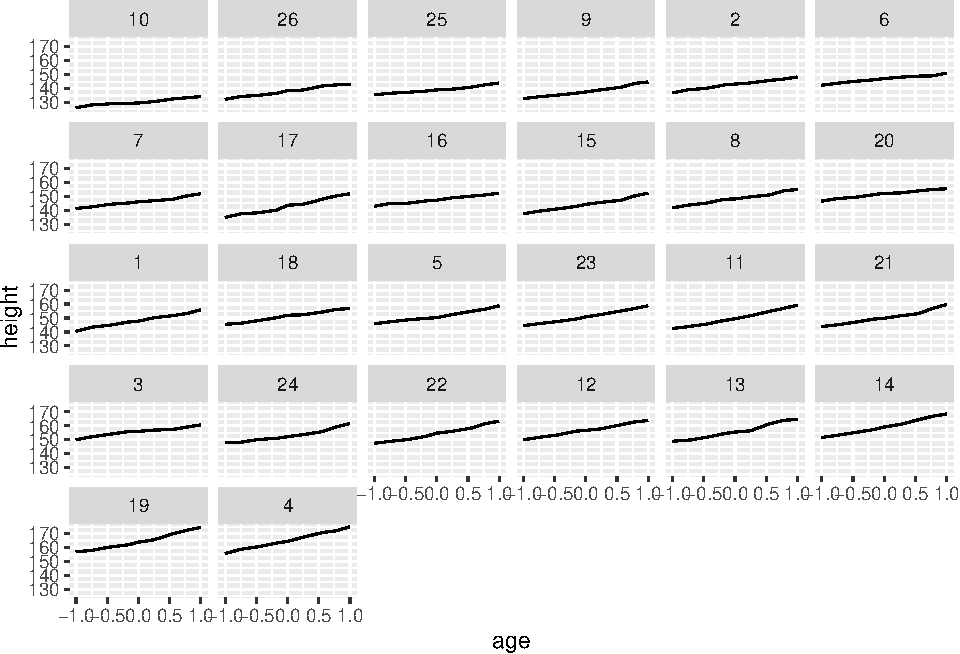
\includegraphics{Introduction-to-R,-Rstudio,-and-ggplot2_files/figure-latex/unnamed-chunk-38-1.pdf}

\hypertarget{themes}{%
\subsection{Themes}\label{themes}}

``Themes are a powerful way to \textbf{customize} the non-data components of your plots: i.e.~titles, labels, fonts, background, gridlines, and legends.'' More details are available at \url{https://ggplot2.tidyverse.org/reference/theme.html}

\begin{Shaded}
\begin{Highlighting}[]
\KeywordTok{ggplot}\NormalTok{(mpg, }\KeywordTok{aes}\NormalTok{(}\DataTypeTok{x =}\NormalTok{ hwy, }\DataTypeTok{y =}\NormalTok{ cty)) }\OperatorTok{+}\StringTok{ }\KeywordTok{geom_point}\NormalTok{() }
\end{Highlighting}
\end{Shaded}

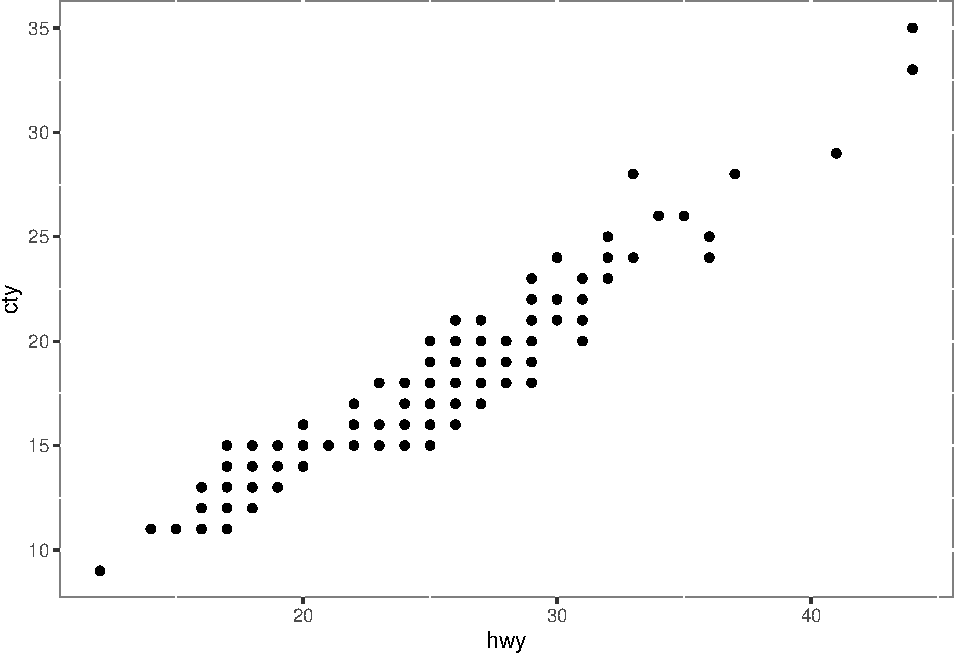
\includegraphics{Introduction-to-R,-Rstudio,-and-ggplot2_files/figure-latex/unnamed-chunk-39-1.pdf}

\begin{Shaded}
\begin{Highlighting}[]
\KeywordTok{ggplot}\NormalTok{(mpg, }\KeywordTok{aes}\NormalTok{(}\DataTypeTok{x =}\NormalTok{ hwy, }\DataTypeTok{y =}\NormalTok{ cty)) }\OperatorTok{+}\StringTok{ }\KeywordTok{geom_point}\NormalTok{() }\OperatorTok{+}\StringTok{ }\KeywordTok{theme}\NormalTok{(}\DataTypeTok{panel.background =} \KeywordTok{element_rect}\NormalTok{(}\DataTypeTok{fill =} \StringTok{"white"}\NormalTok{, }\DataTypeTok{colour =} \StringTok{"grey50"}\NormalTok{))}
\end{Highlighting}
\end{Shaded}

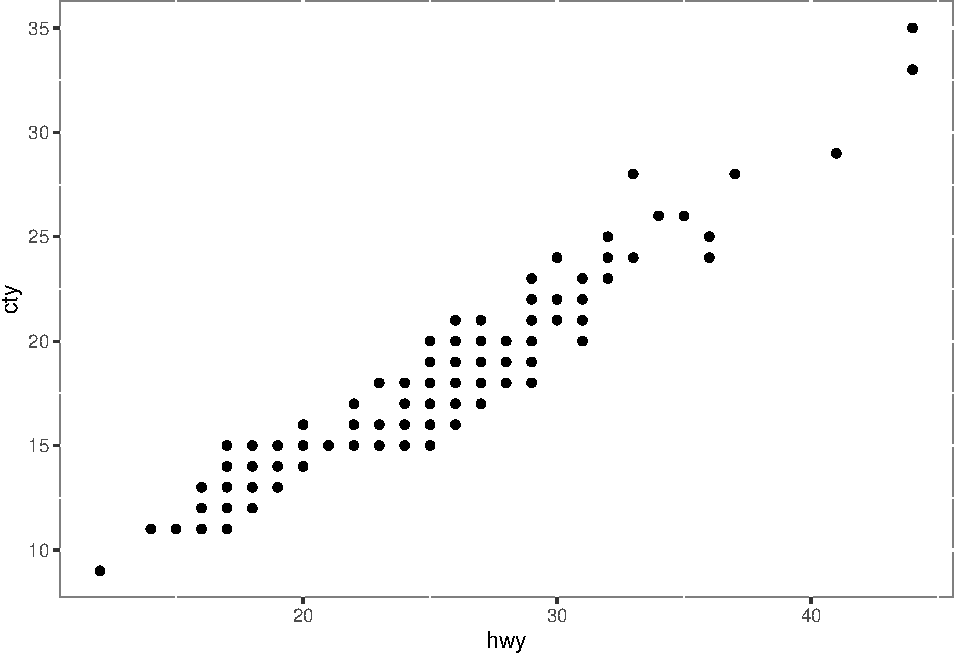
\includegraphics{Introduction-to-R,-Rstudio,-and-ggplot2_files/figure-latex/unnamed-chunk-40-1.pdf}

\begin{Shaded}
\begin{Highlighting}[]
\KeywordTok{ggplot}\NormalTok{(mpg, }\KeywordTok{aes}\NormalTok{(}\DataTypeTok{x =}\NormalTok{ hwy, }\DataTypeTok{y =}\NormalTok{ cty)) }\OperatorTok{+}\StringTok{ }\KeywordTok{geom_point}\NormalTok{() }\OperatorTok{+}\StringTok{ }\KeywordTok{theme_classic}\NormalTok{()}
\end{Highlighting}
\end{Shaded}

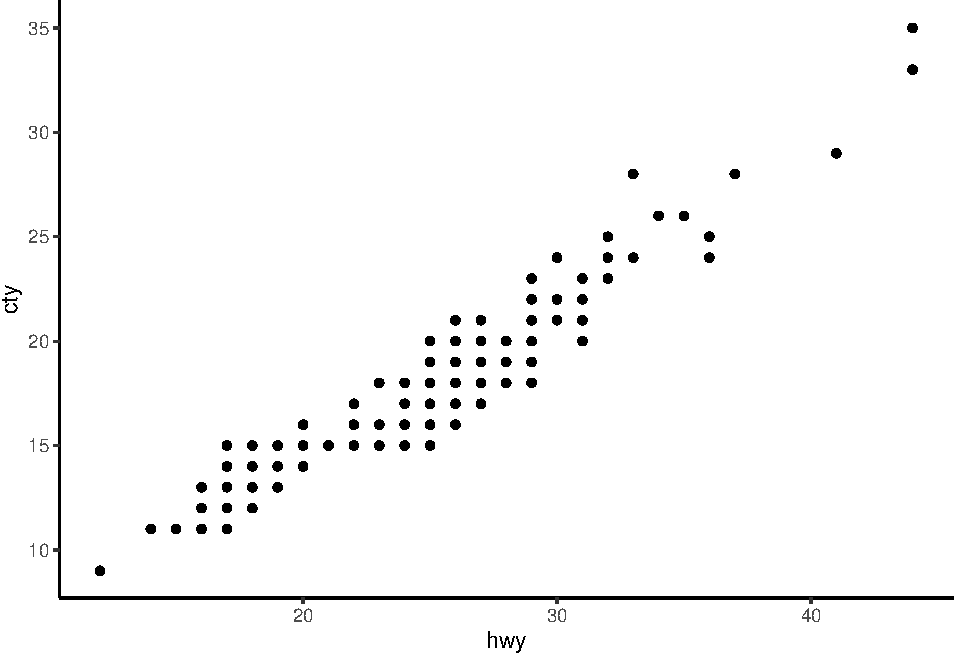
\includegraphics{Introduction-to-R,-Rstudio,-and-ggplot2_files/figure-latex/unnamed-chunk-41-1.pdf}

\hypertarget{saving-a-ggplot}{%
\section{Saving a ggplot}\label{saving-a-ggplot}}

\begin{itemize}
\tightlist
\item
  \texttt{ggsave()} is a convenient function for saving a plot. It defaults to saving the \textbf{last plot} that you displayed.
\end{itemize}

\begin{Shaded}
\begin{Highlighting}[]
\KeywordTok{ggsave}\NormalTok{(}\StringTok{"mtcars.pdf"}\NormalTok{)}
\end{Highlighting}
\end{Shaded}

\begin{verbatim}
## Saving 6.5 x 4.5 in image
\end{verbatim}

\hypertarget{more-resources}{%
\section{More resources}\label{more-resources}}

\begin{itemize}
\tightlist
\item
  \texttt{ggplot2} Reference: \url{https://ggplot2.tidyverse.org/reference/index.html}
\item
  Many R galleries (e.g., \url{https://www.r-graph-gallery.com})
\item
  Google
\end{itemize}

\hypertarget{descriptive-statistics}{%
\chapter{Descriptive Statistics}\label{descriptive-statistics}}

\hypertarget{r-functions-for-descriptive-statistics}{%
\section{R functions for descriptive statistics}\label{r-functions-for-descriptive-statistics}}

\begin{Shaded}
\begin{Highlighting}[]
\CommentTok{# compute mean}
\CommentTok{# we use $ to access `price` variable in the `diamonds` dataset }
\KeywordTok{mean}\NormalTok{(diamonds}\OperatorTok{$}\NormalTok{price)}
\end{Highlighting}
\end{Shaded}

\begin{verbatim}
## [1] 3932.8
\end{verbatim}

\begin{Shaded}
\begin{Highlighting}[]
\CommentTok{# compute median}
\KeywordTok{median}\NormalTok{(diamonds}\OperatorTok{$}\NormalTok{price)}
\end{Highlighting}
\end{Shaded}

\begin{verbatim}
## [1] 2401
\end{verbatim}

\begin{Shaded}
\begin{Highlighting}[]
\CommentTok{# compute variance}
\KeywordTok{var}\NormalTok{(diamonds}\OperatorTok{$}\NormalTok{price)}
\end{Highlighting}
\end{Shaded}

\begin{verbatim}
## [1] 15915629
\end{verbatim}

\begin{Shaded}
\begin{Highlighting}[]
\CommentTok{# compute standard deviation}
\KeywordTok{sd}\NormalTok{(diamonds}\OperatorTok{$}\NormalTok{price)}
\end{Highlighting}
\end{Shaded}

\begin{verbatim}
## [1] 3989.44
\end{verbatim}

\begin{Shaded}
\begin{Highlighting}[]
\CommentTok{# summary of a data frame}
\KeywordTok{summary}\NormalTok{(diamonds)}
\end{Highlighting}
\end{Shaded}

\begin{verbatim}
##      carat               cut        color        clarity     
##  Min.   :0.2000   Fair     : 1610   D: 6775   SI1    :13065  
##  1st Qu.:0.4000   Good     : 4906   E: 9797   VS2    :12258  
##  Median :0.7000   Very Good:12082   F: 9542   SI2    : 9194  
##  Mean   :0.7979   Premium  :13791   G:11292   VS1    : 8171  
##  3rd Qu.:1.0400   Ideal    :21551   H: 8304   VVS2   : 5066  
##  Max.   :5.0100                     I: 5422   VVS1   : 3655  
##                                     J: 2808   (Other): 2531  
##      depth           table           price             x         
##  Min.   :43.00   Min.   :43.00   Min.   :  326   Min.   : 0.000  
##  1st Qu.:61.00   1st Qu.:56.00   1st Qu.:  950   1st Qu.: 4.710  
##  Median :61.80   Median :57.00   Median : 2401   Median : 5.700  
##  Mean   :61.75   Mean   :57.46   Mean   : 3933   Mean   : 5.731  
##  3rd Qu.:62.50   3rd Qu.:59.00   3rd Qu.: 5324   3rd Qu.: 6.540  
##  Max.   :79.00   Max.   :95.00   Max.   :18823   Max.   :10.740  
##                                                                  
##        y                z         
##  Min.   : 0.000   Min.   : 0.000  
##  1st Qu.: 4.720   1st Qu.: 2.910  
##  Median : 5.710   Median : 3.530  
##  Mean   : 5.735   Mean   : 3.539  
##  3rd Qu.: 6.540   3rd Qu.: 4.040  
##  Max.   :58.900   Max.   :31.800  
## 
\end{verbatim}

\hypertarget{qplot}{%
\section{qplot()}\label{qplot}}

\texttt{qplot()}, short for \textbf{quick plot} is a function in the \texttt{ggplot2} package. qplot makes it easy to produce complex plots, often requiring several lines of code using other plotting systems, \textbf{in one line}.

\hypertarget{scatterplots}{%
\section{Scatterplots}\label{scatterplots}}

\begin{Shaded}
\begin{Highlighting}[]
\KeywordTok{ggplot}\NormalTok{(}\DataTypeTok{data =}\NormalTok{ mpg, }\KeywordTok{aes}\NormalTok{(}\DataTypeTok{x =}\NormalTok{ displ, }\DataTypeTok{y =}\NormalTok{ hwy)) }\OperatorTok{+}\StringTok{ }\KeywordTok{geom_point}\NormalTok{()}
\end{Highlighting}
\end{Shaded}

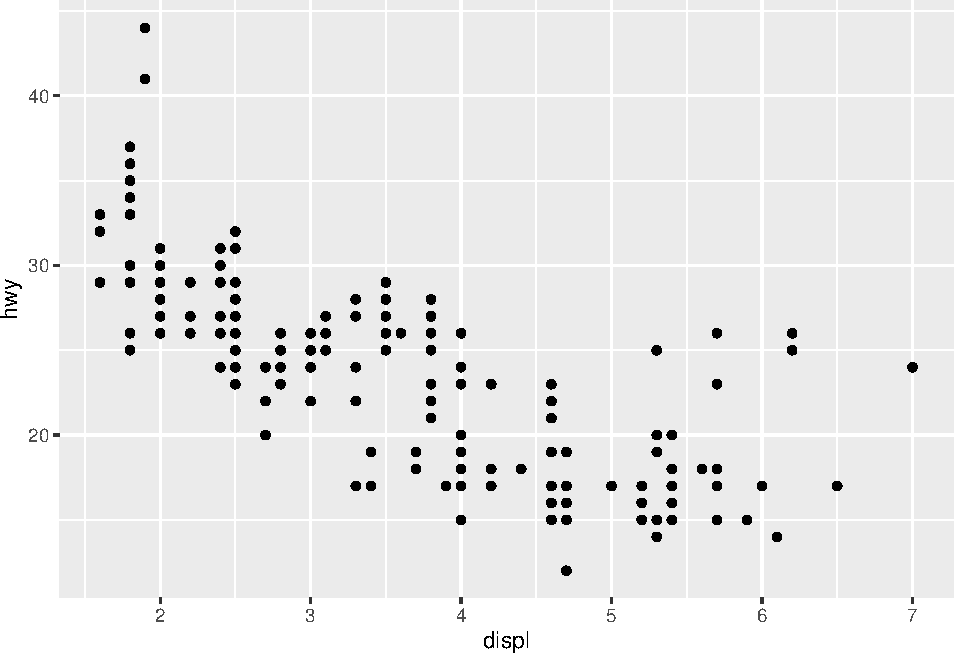
\includegraphics{Introduction-to-R,-Rstudio,-and-ggplot2_files/figure-latex/unnamed-chunk-48-1.pdf}

\begin{Shaded}
\begin{Highlighting}[]
\KeywordTok{qplot}\NormalTok{(displ, hwy, }\DataTypeTok{data =}\NormalTok{ mpg)}
\end{Highlighting}
\end{Shaded}

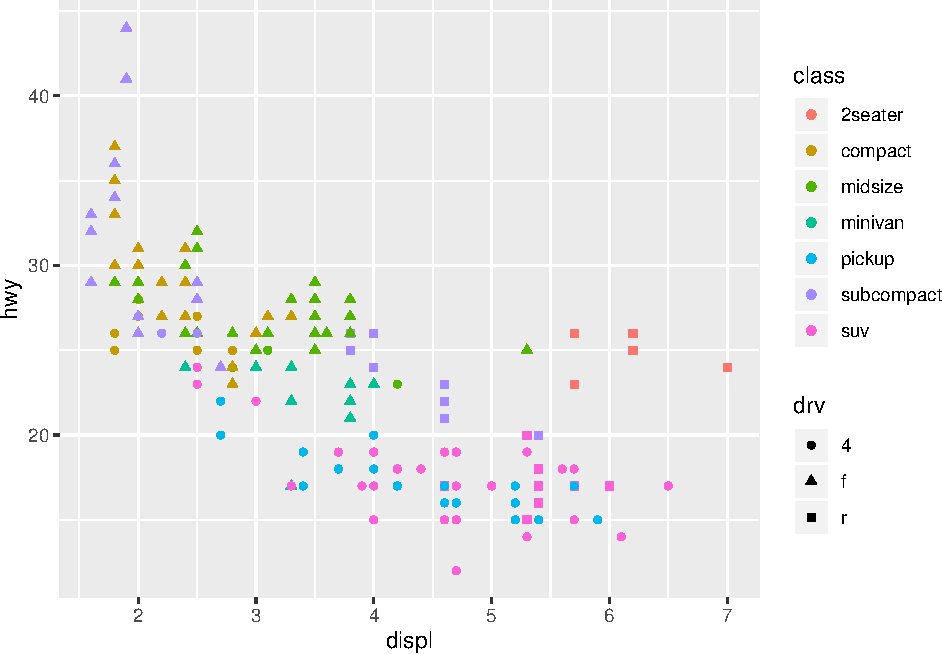
\includegraphics{Introduction-to-R,-Rstudio,-and-ggplot2_files/figure-latex/unnamed-chunk-49-1.pdf}

\begin{Shaded}
\begin{Highlighting}[]
\KeywordTok{ggplot}\NormalTok{(}\DataTypeTok{data =}\NormalTok{ mpg, }\KeywordTok{aes}\NormalTok{(}\DataTypeTok{x =}\NormalTok{ displ, }\DataTypeTok{y =}\NormalTok{ hwy, }\DataTypeTok{color =}\NormalTok{ class)) }\OperatorTok{+}\StringTok{ }\KeywordTok{geom_point}\NormalTok{()}
\end{Highlighting}
\end{Shaded}

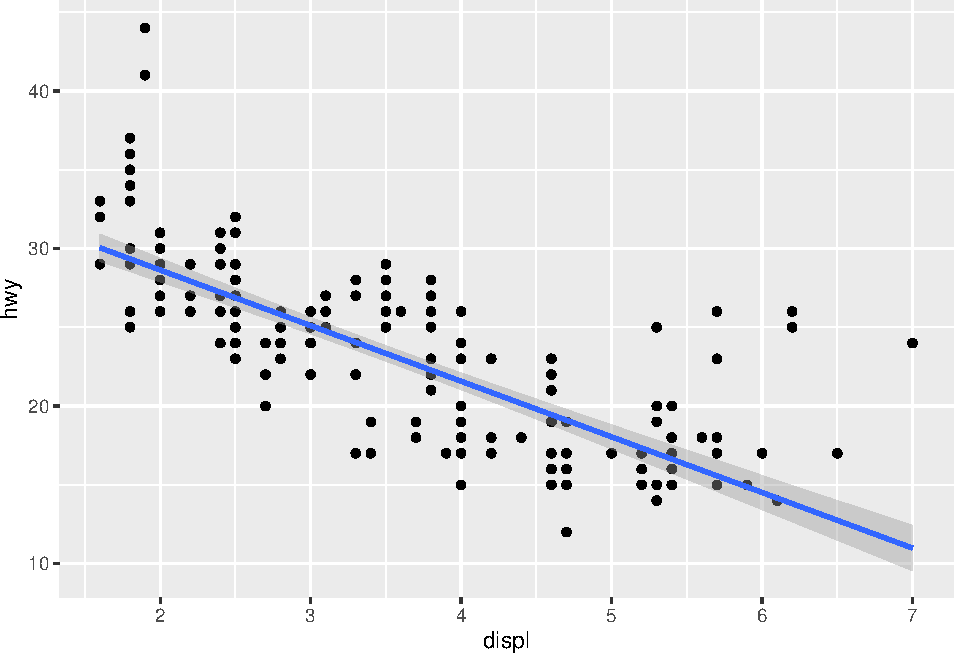
\includegraphics{Introduction-to-R,-Rstudio,-and-ggplot2_files/figure-latex/unnamed-chunk-50-1.pdf}

\begin{Shaded}
\begin{Highlighting}[]
\KeywordTok{qplot}\NormalTok{(displ, hwy, }\DataTypeTok{data =}\NormalTok{ mpg, }\DataTypeTok{color =}\NormalTok{ class)}
\end{Highlighting}
\end{Shaded}

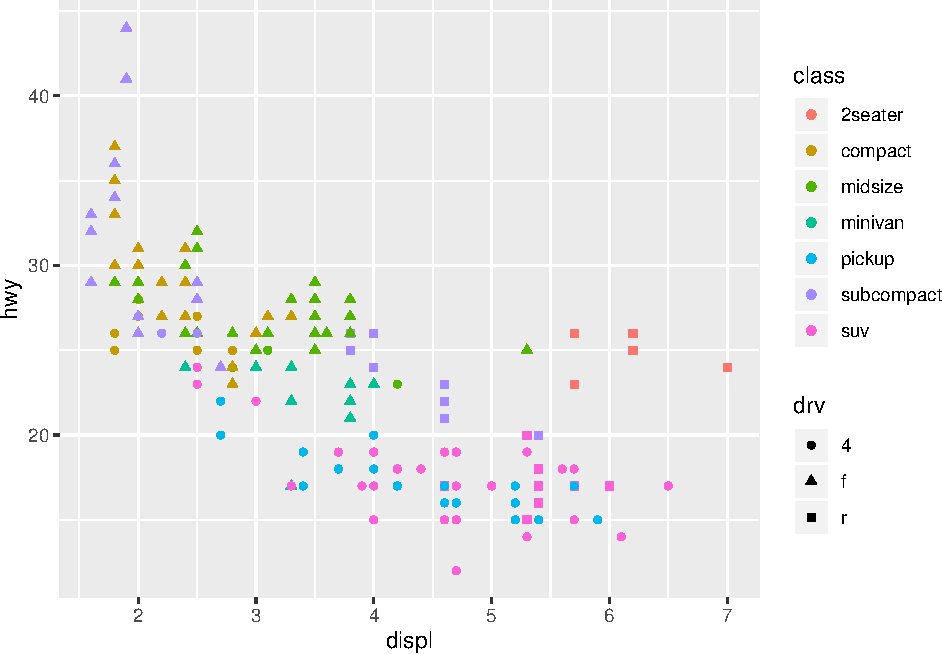
\includegraphics{Introduction-to-R,-Rstudio,-and-ggplot2_files/figure-latex/unnamed-chunk-51-1.pdf}

\begin{Shaded}
\begin{Highlighting}[]
\KeywordTok{ggplot}\NormalTok{(}\DataTypeTok{data =}\NormalTok{ mpg, }\KeywordTok{aes}\NormalTok{(}\DataTypeTok{x =}\NormalTok{ displ, }\DataTypeTok{y =}\NormalTok{ hwy, }\DataTypeTok{color =}\NormalTok{ class, }\DataTypeTok{shape =}\NormalTok{ drv)) }\OperatorTok{+}\StringTok{ }\KeywordTok{geom_point}\NormalTok{()}
\end{Highlighting}
\end{Shaded}

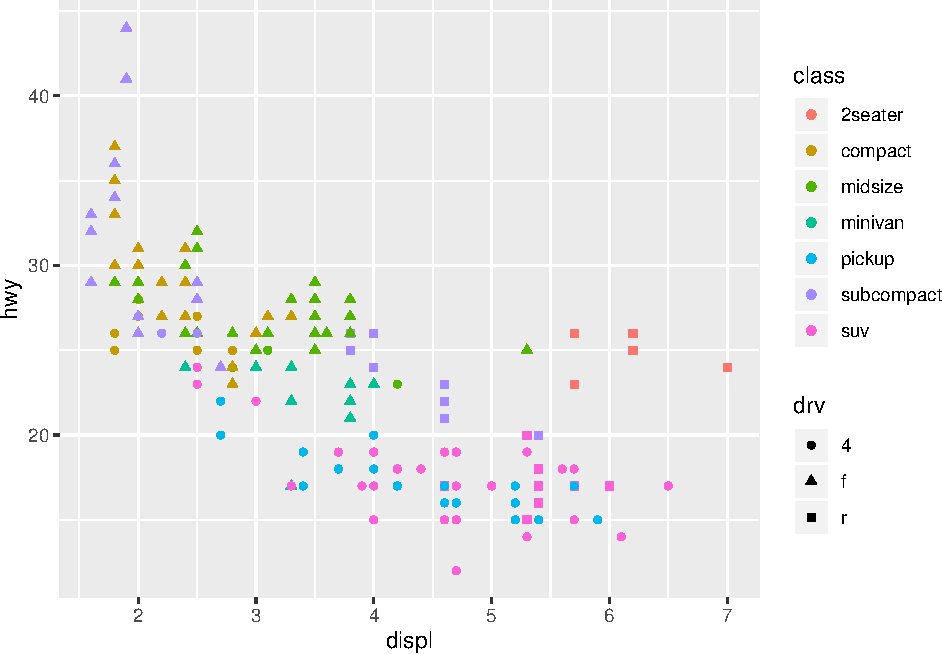
\includegraphics{Introduction-to-R,-Rstudio,-and-ggplot2_files/figure-latex/unnamed-chunk-52-1.pdf}

\begin{Shaded}
\begin{Highlighting}[]
\KeywordTok{qplot}\NormalTok{(displ, hwy, }\DataTypeTok{data =}\NormalTok{ mpg, }\DataTypeTok{color =}\NormalTok{ class, }\DataTypeTok{shape =}\NormalTok{ drv)}
\end{Highlighting}
\end{Shaded}

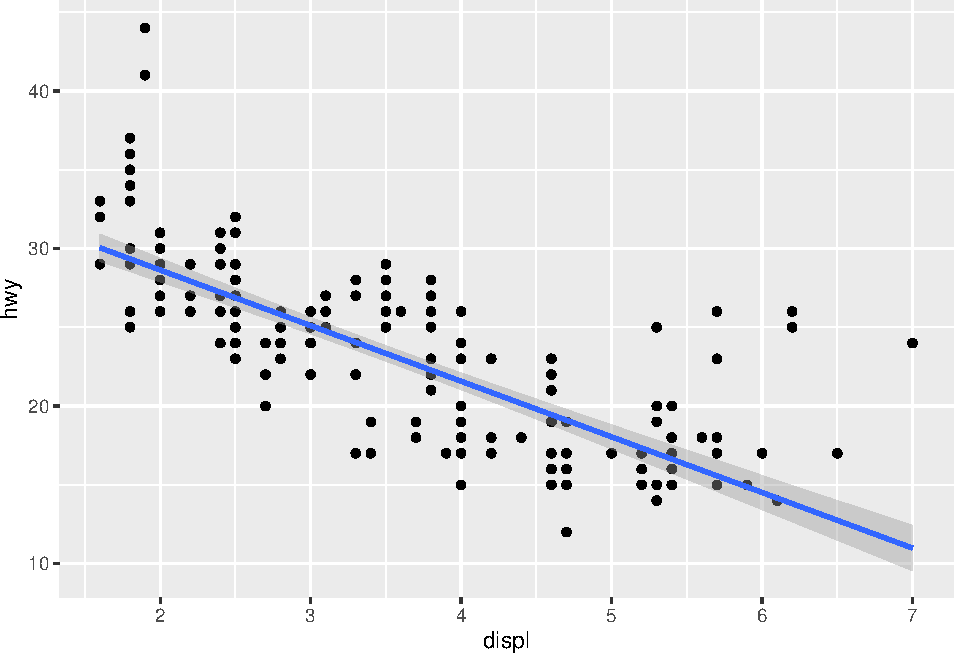
\includegraphics{Introduction-to-R,-Rstudio,-and-ggplot2_files/figure-latex/unnamed-chunk-53-1.pdf}

\begin{Shaded}
\begin{Highlighting}[]
\KeywordTok{ggplot}\NormalTok{(}\DataTypeTok{data =}\NormalTok{ mpg, }\KeywordTok{aes}\NormalTok{(}\DataTypeTok{x =}\NormalTok{ displ, }\DataTypeTok{y =}\NormalTok{ hwy)) }\OperatorTok{+}\StringTok{ }\KeywordTok{geom_point}\NormalTok{() }\OperatorTok{+}\StringTok{ }\KeywordTok{geom_smooth}\NormalTok{(}\DataTypeTok{method =} \StringTok{"lm"}\NormalTok{)}
\end{Highlighting}
\end{Shaded}

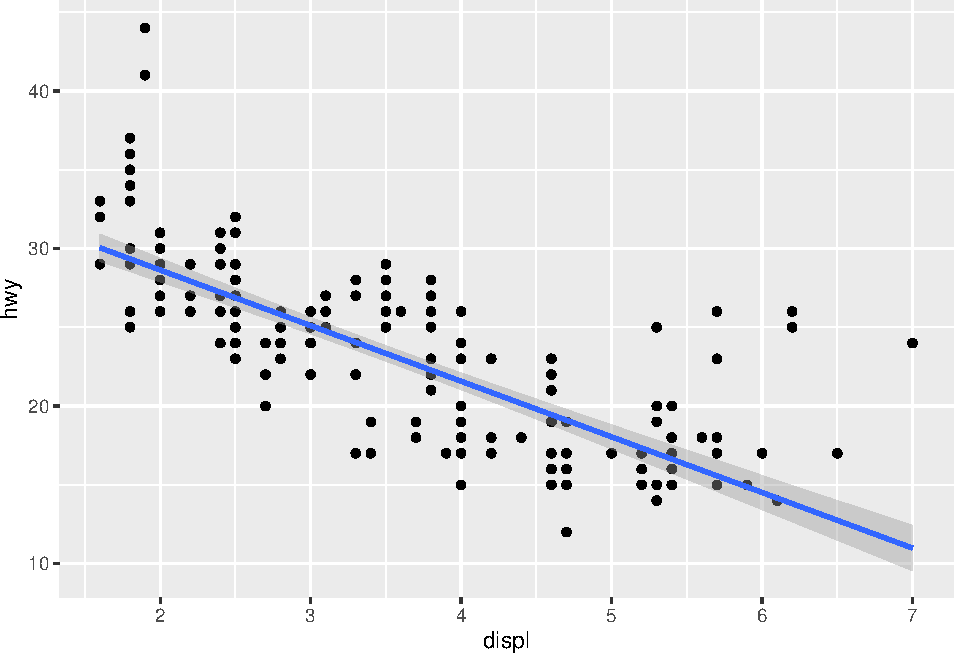
\includegraphics{Introduction-to-R,-Rstudio,-and-ggplot2_files/figure-latex/unnamed-chunk-54-1.pdf}

\begin{Shaded}
\begin{Highlighting}[]
\KeywordTok{qplot}\NormalTok{(displ, hwy, }\DataTypeTok{data =}\NormalTok{ mpg, }\DataTypeTok{geom =} \KeywordTok{c}\NormalTok{(}\StringTok{"point"}\NormalTok{, }\StringTok{"smooth"}\NormalTok{)) }
\end{Highlighting}
\end{Shaded}

\begin{verbatim}
## `geom_smooth()` using method = 'loess' and formula 'y ~ x'
\end{verbatim}

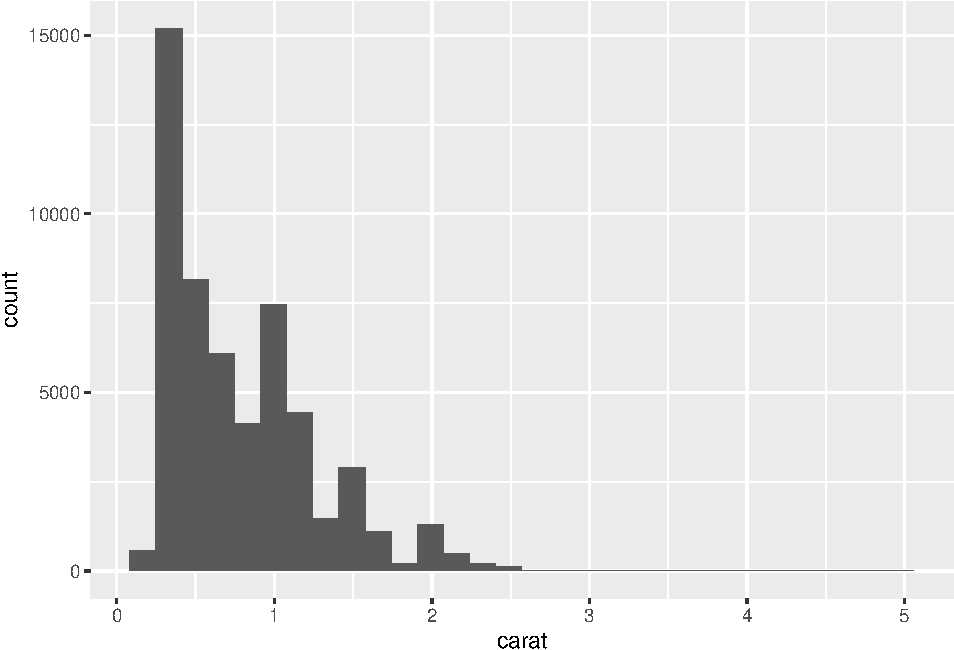
\includegraphics{Introduction-to-R,-Rstudio,-and-ggplot2_files/figure-latex/unnamed-chunk-55-1.pdf}

\hypertarget{histogram}{%
\section{Histogram}\label{histogram}}

\begin{Shaded}
\begin{Highlighting}[]
\KeywordTok{ggplot}\NormalTok{(}\DataTypeTok{data =}\NormalTok{ diamonds, }\KeywordTok{aes}\NormalTok{(}\DataTypeTok{x =}\NormalTok{ carat)) }\OperatorTok{+}\StringTok{ }\KeywordTok{geom_histogram}\NormalTok{()}
\end{Highlighting}
\end{Shaded}

\begin{verbatim}
## `stat_bin()` using `bins = 30`. Pick better value with `binwidth`.
\end{verbatim}

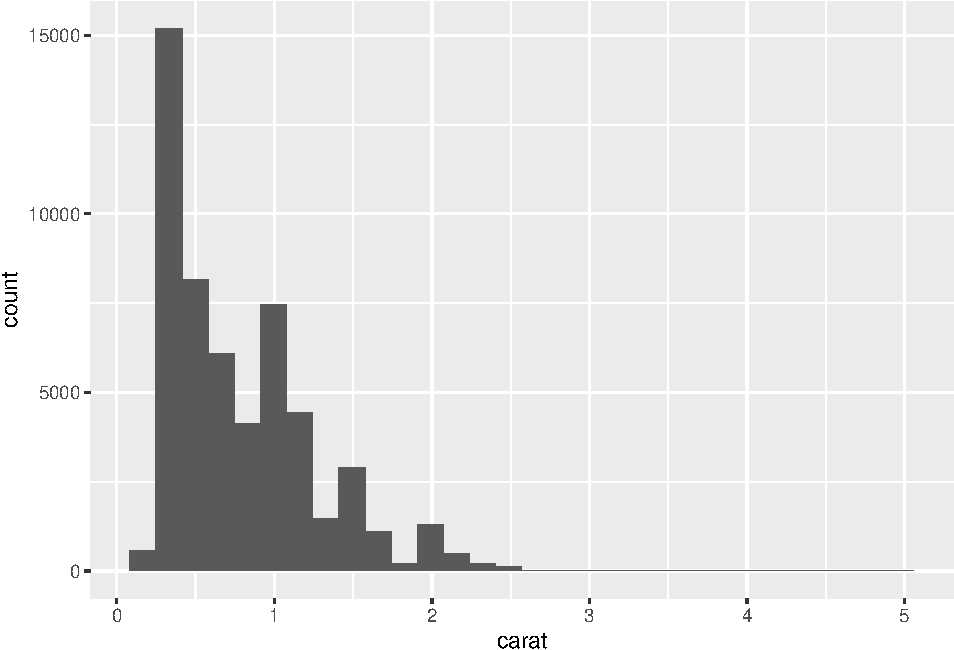
\includegraphics{Introduction-to-R,-Rstudio,-and-ggplot2_files/figure-latex/unnamed-chunk-56-1.pdf}

\begin{Shaded}
\begin{Highlighting}[]
\KeywordTok{qplot}\NormalTok{(carat, }\DataTypeTok{data =}\NormalTok{ diamonds, }\DataTypeTok{geom =} \StringTok{"histogram"}\NormalTok{)}
\end{Highlighting}
\end{Shaded}

\begin{verbatim}
## `stat_bin()` using `bins = 30`. Pick better value with `binwidth`.
\end{verbatim}

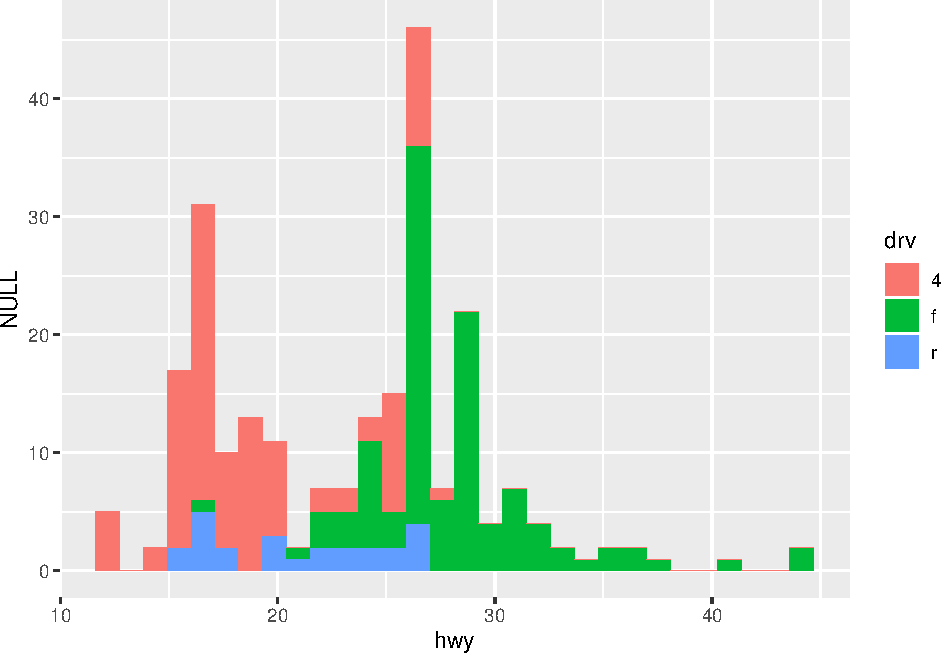
\includegraphics{Introduction-to-R,-Rstudio,-and-ggplot2_files/figure-latex/unnamed-chunk-57-1.pdf}

\begin{Shaded}
\begin{Highlighting}[]
\KeywordTok{ggplot}\NormalTok{(}\DataTypeTok{data =}\NormalTok{ diamonds, }\KeywordTok{aes}\NormalTok{(}\DataTypeTok{x =}\NormalTok{ carat)) }\OperatorTok{+}\StringTok{ }\KeywordTok{geom_histogram}\NormalTok{(}\DataTypeTok{binwidth =} \FloatTok{0.05}\NormalTok{) }\OperatorTok{+}\StringTok{ }\KeywordTok{xlim}\NormalTok{(}\KeywordTok{c}\NormalTok{(}\DecValTok{0}\NormalTok{,}\DecValTok{3}\NormalTok{))}
\end{Highlighting}
\end{Shaded}

\begin{verbatim}
## Warning: Removed 32 rows containing non-finite values (stat_bin).
\end{verbatim}

\begin{verbatim}
## Warning: Removed 2 rows containing missing values (geom_bar).
\end{verbatim}

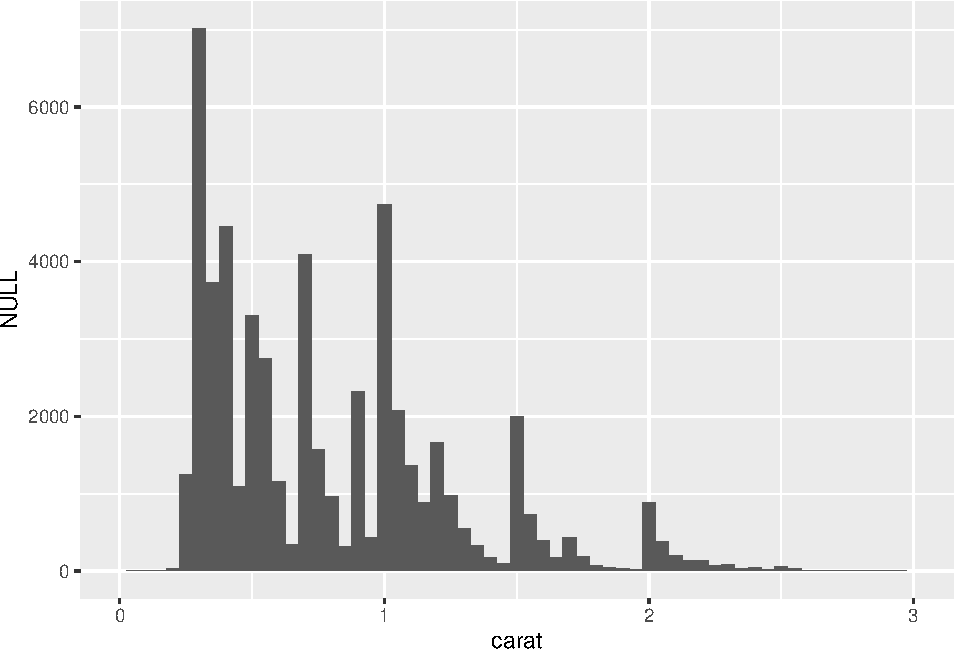
\includegraphics{Introduction-to-R,-Rstudio,-and-ggplot2_files/figure-latex/unnamed-chunk-58-1.pdf}

\begin{Shaded}
\begin{Highlighting}[]
\KeywordTok{qplot}\NormalTok{(carat, }\DataTypeTok{data =}\NormalTok{ diamonds, }\DataTypeTok{geom =} \StringTok{"histogram"}\NormalTok{, }\DataTypeTok{binwidth =} \FloatTok{0.05}\NormalTok{, }\DataTypeTok{xlim =} \KeywordTok{c}\NormalTok{(}\DecValTok{0}\NormalTok{,}\DecValTok{3}\NormalTok{))}
\end{Highlighting}
\end{Shaded}

\begin{verbatim}
## Warning: Removed 32 rows containing non-finite values (stat_bin).
\end{verbatim}

\begin{verbatim}
## Warning: Removed 2 rows containing missing values (geom_bar).
\end{verbatim}

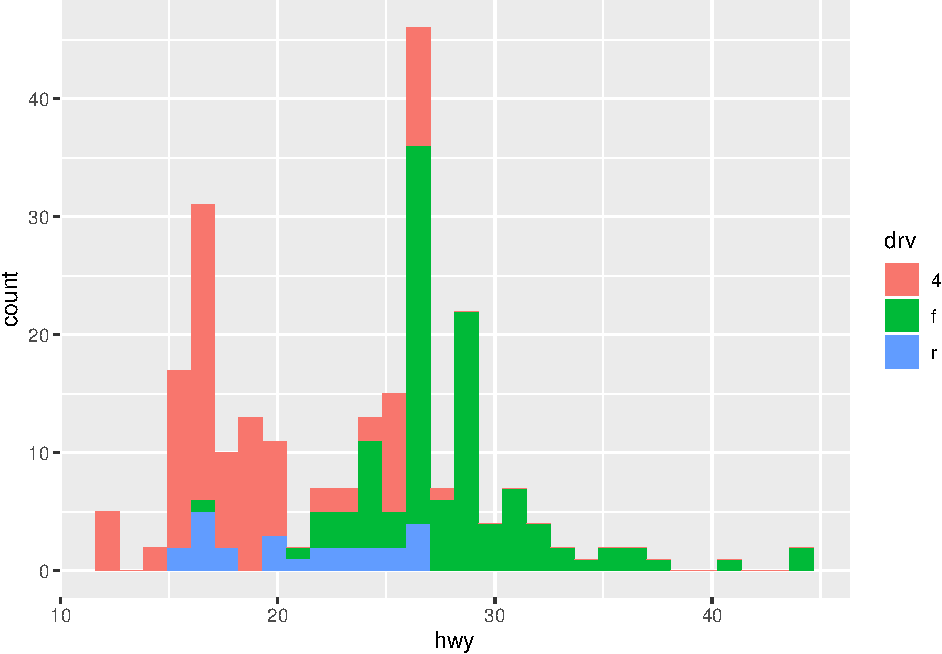
\includegraphics{Introduction-to-R,-Rstudio,-and-ggplot2_files/figure-latex/unnamed-chunk-59-1.pdf}

\begin{Shaded}
\begin{Highlighting}[]
\KeywordTok{ggplot}\NormalTok{(}\DataTypeTok{data =}\NormalTok{ mpg, }\KeywordTok{aes}\NormalTok{(}\DataTypeTok{x =}\NormalTok{ hwy, }\DataTypeTok{fill =}\NormalTok{ drv)) }\OperatorTok{+}\StringTok{ }\KeywordTok{geom_histogram}\NormalTok{() }
\end{Highlighting}
\end{Shaded}

\begin{verbatim}
## `stat_bin()` using `bins = 30`. Pick better value with `binwidth`.
\end{verbatim}

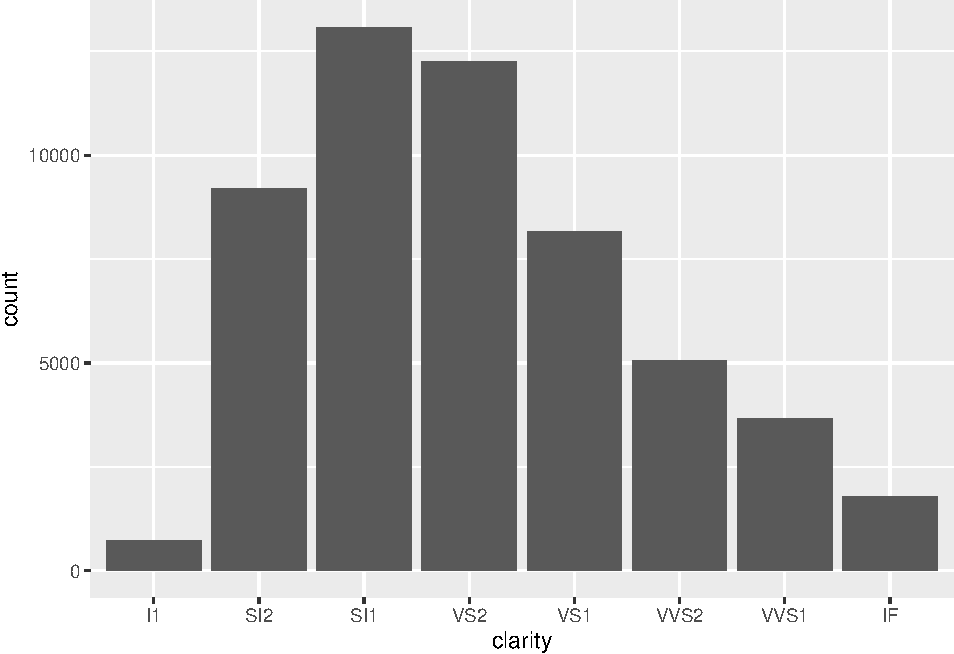
\includegraphics{Introduction-to-R,-Rstudio,-and-ggplot2_files/figure-latex/unnamed-chunk-60-1.pdf}

\begin{Shaded}
\begin{Highlighting}[]
\KeywordTok{qplot}\NormalTok{(hwy, }\DataTypeTok{data =}\NormalTok{ mpg, }\DataTypeTok{geom =} \StringTok{"histogram"}\NormalTok{, }\DataTypeTok{fill =}\NormalTok{ drv)}
\end{Highlighting}
\end{Shaded}

\begin{verbatim}
## `stat_bin()` using `bins = 30`. Pick better value with `binwidth`.
\end{verbatim}

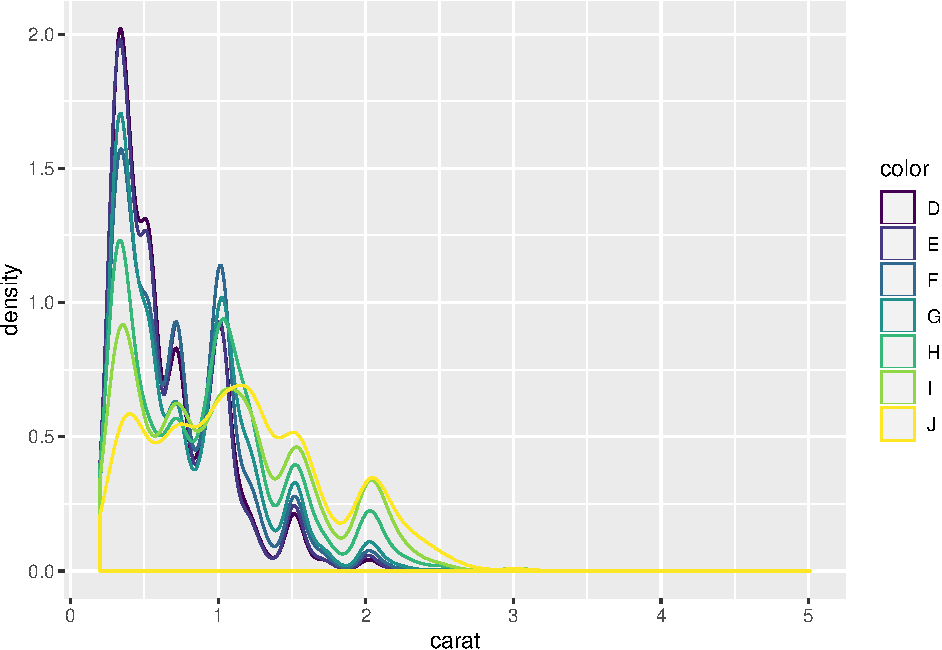
\includegraphics{Introduction-to-R,-Rstudio,-and-ggplot2_files/figure-latex/unnamed-chunk-61-1.pdf}

\hypertarget{density-plots}{%
\section{Density plots}\label{density-plots}}

\begin{Shaded}
\begin{Highlighting}[]
\KeywordTok{ggplot}\NormalTok{(}\DataTypeTok{data =}\NormalTok{ diamonds, }\KeywordTok{aes}\NormalTok{(}\DataTypeTok{x =}\NormalTok{ carat, }\DataTypeTok{color =}\NormalTok{ color)) }\OperatorTok{+}\StringTok{ }\KeywordTok{geom_density}\NormalTok{() }
\end{Highlighting}
\end{Shaded}

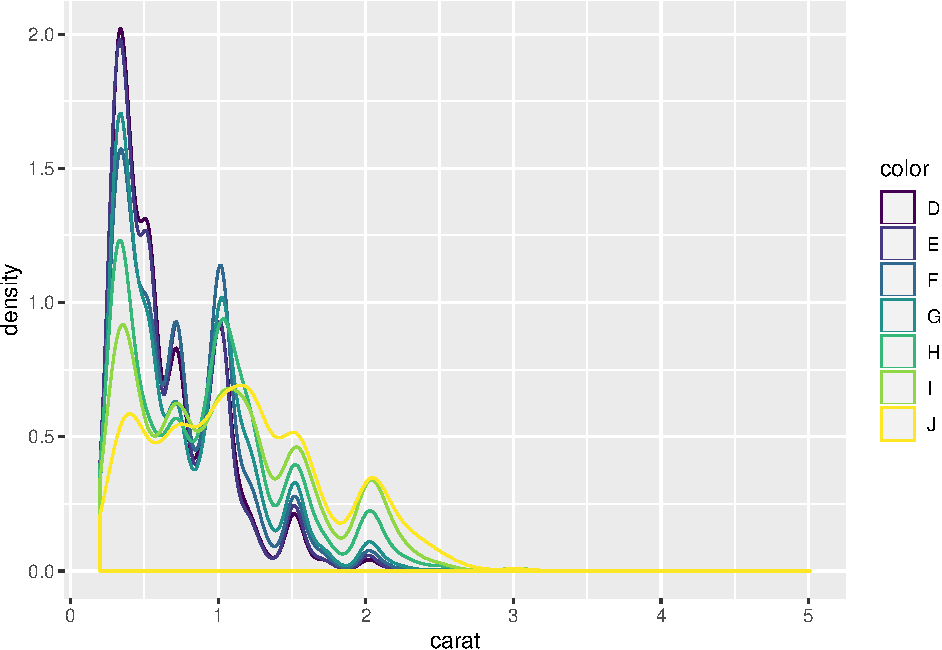
\includegraphics{Introduction-to-R,-Rstudio,-and-ggplot2_files/figure-latex/unnamed-chunk-62-1.pdf}

\begin{Shaded}
\begin{Highlighting}[]
\KeywordTok{qplot}\NormalTok{(carat, }\DataTypeTok{data =}\NormalTok{ diamonds, }\DataTypeTok{geom =} \StringTok{"density"}\NormalTok{, }\DataTypeTok{color =}\NormalTok{ color)}
\end{Highlighting}
\end{Shaded}

\includegraphics{Introduction-to-R,-Rstudio,-and-ggplot2_files/figure-latex/unnamed-chunk-63-1.pdf}

\hypertarget{barplots}{%
\section{Barplots}\label{barplots}}

\begin{Shaded}
\begin{Highlighting}[]
\KeywordTok{ggplot}\NormalTok{(}\DataTypeTok{data =}\NormalTok{ diamonds, }\KeywordTok{aes}\NormalTok{(}\DataTypeTok{x =}\NormalTok{ clarity)) }\OperatorTok{+}\StringTok{ }\KeywordTok{geom_bar}\NormalTok{() }
\end{Highlighting}
\end{Shaded}

\includegraphics{Introduction-to-R,-Rstudio,-and-ggplot2_files/figure-latex/unnamed-chunk-64-1.pdf}

\begin{Shaded}
\begin{Highlighting}[]
\KeywordTok{qplot}\NormalTok{(clarity, }\DataTypeTok{data =}\NormalTok{ diamonds, }\DataTypeTok{geom =} \StringTok{"bar"}\NormalTok{)}
\end{Highlighting}
\end{Shaded}

\includegraphics{Introduction-to-R,-Rstudio,-and-ggplot2_files/figure-latex/unnamed-chunk-65-1.pdf}

\begin{Shaded}
\begin{Highlighting}[]
\KeywordTok{ggplot}\NormalTok{(}\DataTypeTok{data =}\NormalTok{ diamonds, }\KeywordTok{aes}\NormalTok{(}\DataTypeTok{x =}\NormalTok{ clarity, }\DataTypeTok{fill =}\NormalTok{ cut)) }\OperatorTok{+}\StringTok{ }\KeywordTok{geom_bar}\NormalTok{() }
\end{Highlighting}
\end{Shaded}

\includegraphics{Introduction-to-R,-Rstudio,-and-ggplot2_files/figure-latex/unnamed-chunk-66-1.pdf}

\begin{Shaded}
\begin{Highlighting}[]
\KeywordTok{qplot}\NormalTok{(clarity, }\DataTypeTok{data =}\NormalTok{ diamonds, }\DataTypeTok{geom =} \StringTok{"bar"}\NormalTok{, }\DataTypeTok{fill =}\NormalTok{ cut)}
\end{Highlighting}
\end{Shaded}

\includegraphics{Introduction-to-R,-Rstudio,-and-ggplot2_files/figure-latex/unnamed-chunk-67-1.pdf}

\hypertarget{boxplots}{%
\section{Boxplots}\label{boxplots}}

\begin{Shaded}
\begin{Highlighting}[]
\KeywordTok{ggplot}\NormalTok{(}\DataTypeTok{data =}\NormalTok{ diamonds, }\KeywordTok{aes}\NormalTok{(}\DataTypeTok{y =}\NormalTok{ price)) }\OperatorTok{+}\StringTok{ }\KeywordTok{geom_boxplot}\NormalTok{() }
\end{Highlighting}
\end{Shaded}

\includegraphics{Introduction-to-R,-Rstudio,-and-ggplot2_files/figure-latex/unnamed-chunk-68-1.pdf}

\begin{Shaded}
\begin{Highlighting}[]
\KeywordTok{qplot}\NormalTok{(}\DataTypeTok{y =}\NormalTok{ price, }\DataTypeTok{data =}\NormalTok{ diamonds, }\DataTypeTok{geom =} \StringTok{"boxplot"}\NormalTok{)}
\end{Highlighting}
\end{Shaded}

\includegraphics{Introduction-to-R,-Rstudio,-and-ggplot2_files/figure-latex/unnamed-chunk-69-1.pdf}

\begin{Shaded}
\begin{Highlighting}[]
\KeywordTok{ggplot}\NormalTok{(}\DataTypeTok{data =}\NormalTok{ diamonds, }\KeywordTok{aes}\NormalTok{(}\DataTypeTok{x =}\NormalTok{ cut, }\DataTypeTok{y =}\NormalTok{ price)) }\OperatorTok{+}\StringTok{ }\KeywordTok{geom_boxplot}\NormalTok{() }
\end{Highlighting}
\end{Shaded}

\includegraphics{Introduction-to-R,-Rstudio,-and-ggplot2_files/figure-latex/unnamed-chunk-70-1.pdf}

\hypertarget{faceting}{%
\section{Faceting}\label{faceting}}

\begin{Shaded}
\begin{Highlighting}[]
\KeywordTok{ggplot}\NormalTok{(}\DataTypeTok{data =}\NormalTok{ diamonds, }\KeywordTok{aes}\NormalTok{(}\DataTypeTok{x =}\NormalTok{ carat, }\DataTypeTok{y =}\NormalTok{ price)) }\OperatorTok{+}\StringTok{ }\KeywordTok{geom_point}\NormalTok{() }\OperatorTok{+}\StringTok{ }\KeywordTok{facet_grid}\NormalTok{(cut }\OperatorTok{~}\StringTok{ }\NormalTok{color)}
\end{Highlighting}
\end{Shaded}

\includegraphics{Introduction-to-R,-Rstudio,-and-ggplot2_files/figure-latex/unnamed-chunk-71-1.pdf}

\begin{Shaded}
\begin{Highlighting}[]
\KeywordTok{qplot}\NormalTok{(carat, price, }\DataTypeTok{data =}\NormalTok{ diamonds, }\DataTypeTok{facets =}\NormalTok{ cut }\OperatorTok{~}\StringTok{ }\NormalTok{color)}
\end{Highlighting}
\end{Shaded}

\includegraphics{Introduction-to-R,-Rstudio,-and-ggplot2_files/figure-latex/unnamed-chunk-72-1.pdf}

\hypertarget{the-corrplot-package}{%
\section{\texorpdfstring{The \texttt{corrplot} Package}{The corrplot Package}}\label{the-corrplot-package}}

\begin{itemize}
\tightlist
\item
  \url{https://cran.r-project.org/web/packages/corrplot/vignettes/corrplot-intro.html}
\item
  ``The corrplot package is a graphical display of a \textbf{correlation matrix}, confidence interval. It also contains some algorithms to do matrix reordering. In addition, corrplot is good at details, including choosing color, text labels, color labels, layout, etc.''
\end{itemize}

\begin{Shaded}
\begin{Highlighting}[]
\KeywordTok{library}\NormalTok{(corrplot)}
\end{Highlighting}
\end{Shaded}

\begin{Shaded}
\begin{Highlighting}[]
\KeywordTok{corrplot.mixed}\NormalTok{(}\KeywordTok{cor}\NormalTok{(mtcars))}
\end{Highlighting}
\end{Shaded}

\includegraphics{Introduction-to-R,-Rstudio,-and-ggplot2_files/figure-latex/unnamed-chunk-74-1.pdf}

\hypertarget{exercise}{%
\chapter{Exercise}\label{exercise}}

\begin{itemize}
\tightlist
\item
  Exercise 1: \texttt{midwest} is a dataset in \texttt{ggplot2}, and contains demographic information of midwest counties. Replicate the following scatterplot as close as you can. The variable for the x-axis, y-axis, color aesthetic, size aesthetic are \texttt{area}, \texttt{poptotal}, \texttt{state}, and \texttt{popdensity}.
\end{itemize}

\includegraphics{practice1.png}

\begin{itemize}
\tightlist
\item
  Excercise 2: Replicate the following barplot using the \texttt{mpg} dataset. Use \texttt{theme(axis.text.x\ =\ element\_text(angle=65,\ vjust=0.6))}. Check why we need this theme by plotting with and without this theme. You also need \texttt{width\ =\ 0.5} option in a geom to have more space between bar.
\end{itemize}

\includegraphics{practice2.png}

\hypertarget{base-r}{%
\chapter{Base R}\label{base-r}}

\begin{Shaded}
\begin{Highlighting}[]
\KeywordTok{suppressMessages}\NormalTok{(}\KeywordTok{library}\NormalTok{(tidyverse))}
\end{Highlighting}
\end{Shaded}

\hypertarget{topics}{%
\section{Topics}\label{topics}}

\begin{itemize}
\tightlist
\item
  R Objects and Variables
\item
  Data Structure
\item
  Sub-Setting
\item
  Functions
\item
  Control Flow (if, for, while)
\end{itemize}

\hypertarget{further-reading}{%
\section{Further reading}\label{further-reading}}

\begin{itemize}
\tightlist
\item
  Wickham, H. (2014). Advanced R. Chapman and Hall/CRC

  \begin{itemize}
  \tightlist
  \item
    \url{http://adv-r.had.co.nz}
  \item
    This is a nice book to read after you become comfortable in base R (not required in this course)
  \end{itemize}
\end{itemize}

\hypertarget{interaction-with-r}{%
\section{Interaction with R}\label{interaction-with-r}}

\begin{itemize}
\tightlist
\item
  R Console: for easy interactive exploration of ideas
\item
  R Script file (.R): for sequence of R commands
\item
  R markdown (.Rmd): for reproducible and dynamic reports
\end{itemize}

\hypertarget{r-objects-and-variables}{%
\section{R Objects and Variables}\label{r-objects-and-variables}}

\begin{itemize}
\tightlist
\item
  \textbf{Everything in R is stored as an object}, which is associated with a variable name.
\item
  An object is a technical terminology defined in \textbf{Object Oriented Programming (OOP)}. (OOP is an important concept but not in this class)
\item
  A variable name can be assigned to an object using the \textbf{assignment operator}.
\end{itemize}

\begin{Shaded}
\begin{Highlighting}[]
\CommentTok{# store a number to a variable named `a`}
\NormalTok{a <-}\StringTok{ }\FloatTok{0.2}
\end{Highlighting}
\end{Shaded}

\begin{Shaded}
\begin{Highlighting}[]
\CommentTok{# print a}
\NormalTok{a}
\end{Highlighting}
\end{Shaded}

\begin{verbatim}
## [1] 0.2
\end{verbatim}

\begin{Shaded}
\begin{Highlighting}[]
\CommentTok{# store a vector to a variable named `b`}
\NormalTok{b <-}\StringTok{ }\KeywordTok{c}\NormalTok{(}\DecValTok{1}\NormalTok{,}\DecValTok{4}\NormalTok{,}\DecValTok{9}\NormalTok{)}
\end{Highlighting}
\end{Shaded}

\begin{Shaded}
\begin{Highlighting}[]
\CommentTok{# print b}
\NormalTok{b}
\end{Highlighting}
\end{Shaded}

\begin{verbatim}
## [1] 1 4 9
\end{verbatim}

\begin{Shaded}
\begin{Highlighting}[]
\NormalTok{z <-}\StringTok{ }\DecValTok{5}
\NormalTok{i <-}\StringTok{ }\NormalTok{(z }\OperatorTok{*}\StringTok{ }\DecValTok{2} \OperatorTok{+}\StringTok{ }\DecValTok{45}\NormalTok{)}\OperatorTok{/}\DecValTok{2}
\NormalTok{i}
\end{Highlighting}
\end{Shaded}

\begin{verbatim}
## [1] 27.5
\end{verbatim}

\begin{itemize}
\tightlist
\item
  We can think of the assignment operation as ``\textbf{evaluate} whatever is given on the \textbf{right side} of the operator, and assign (store) the result (an object of some type) of this evaluation in the variable whose name is given on the \textbf{left side}
\end{itemize}

\hypertarget{data-structure}{%
\section{Data Structure}\label{data-structure}}

\begin{itemize}
\tightlist
\item
  R has \textbf{base data structures}.
\item
  Almost all other objects are built upon base data structures.
\item
  R base data structures can be organized by their dimensionality:
\end{itemize}

\begin{longtable}[]{@{}lll@{}}
\toprule
Dimension & Homogeneous & Heterogeneous\tabularnewline
\midrule
\endhead
1D & Atomic vector & List\tabularnewline
2D & Matrix & Data frame\tabularnewline
nD & Array &\tabularnewline
\bottomrule
\end{longtable}

\includegraphics{datastructure.png}

\hypertarget{vectors-come-in-two-flavours}{%
\section{Vectors Come in Two Flavours}\label{vectors-come-in-two-flavours}}

\begin{itemize}
\tightlist
\item
  Atomic vectors (homogeneous)

  \begin{itemize}
  \tightlist
  \item
    All elements of an atomic vector \textbf{must be the same type}.
  \item
    There are \textbf{6 types} of an atomic vector

    \begin{itemize}
    \tightlist
    \item
      \textbf{Logical} (TRUE or FALSE), \textbf{integer}, \textbf{double}, and \textbf{character} (+ rarely used \textbf{complex} and \textbf{raw})
    \end{itemize}
  \item
    Atomic vectors are usually created with \texttt{c()}, short for combine:

    \begin{itemize}
    \tightlist
    \item
      \texttt{a\ \textless{}-\ c(TRUE,\ FALSE,\ T,\ F)} \# logical
    \item
      \texttt{a\ \textless{}-\ c(1L,\ 6L,\ 5L)} \# integer
    \item
      \texttt{a\ \textless{}-\ c(1,\ 2.5,\ 3.8)} \# double
    \item
      \texttt{a\ \textless{}-\ c("apple",\ "orange")} \# character
    \end{itemize}
  \end{itemize}
\item
  Lists (heterogeneous)

  \begin{itemize}
  \tightlist
  \item
    Lists are different from atomic vectors because their elements can be of any type.
  \item
    List are created by \texttt{list()}
  \item
    \texttt{\textgreater{}\ x\ \textless{}-\ list(1:3,\ "a",\ c(TRUE,\ FALSE))}
  \end{itemize}
\end{itemize}

\hypertarget{a-vector-has-three-properties}{%
\section{A Vector Has Three Properties}\label{a-vector-has-three-properties}}

\begin{itemize}
\tightlist
\item
  \textbf{Type}: \texttt{typeof()} returns the type of an object.
\end{itemize}

\begin{Shaded}
\begin{Highlighting}[]
\KeywordTok{typeof}\NormalTok{(}\KeywordTok{c}\NormalTok{(}\DecValTok{1}\NormalTok{,}\DecValTok{2}\NormalTok{,}\DecValTok{3}\NormalTok{))}
\end{Highlighting}
\end{Shaded}

\begin{verbatim}
## [1] "double"
\end{verbatim}

\begin{itemize}
\tightlist
\item
  \textbf{Length}: \texttt{length()} returns the number of elements in a vector
\end{itemize}

\begin{Shaded}
\begin{Highlighting}[]
\KeywordTok{length}\NormalTok{(}\KeywordTok{c}\NormalTok{(}\DecValTok{1}\NormalTok{,}\DecValTok{2}\NormalTok{,}\DecValTok{3}\NormalTok{))}
\end{Highlighting}
\end{Shaded}

\begin{verbatim}
## [1] 3
\end{verbatim}

\begin{itemize}
\tightlist
\item
  \textbf{Attributes}: \texttt{attributes()} returns additional arbitrary metadata
\end{itemize}

\begin{Shaded}
\begin{Highlighting}[]
\KeywordTok{attributes}\NormalTok{(}\KeywordTok{c}\NormalTok{(}\DecValTok{1}\NormalTok{,}\DecValTok{2}\NormalTok{,}\DecValTok{3}\NormalTok{))}
\end{Highlighting}
\end{Shaded}

\begin{verbatim}
## NULL
\end{verbatim}

\hypertarget{attributes}{%
\section{Attributes}\label{attributes}}

\begin{itemize}
\tightlist
\item
  All objects can have attributes to store \textbf{metadata} about the object.
\item
  Attributes can be considered as a \textbf{named list}.
\item
  Attributes can be accessed individually with \texttt{attr()} or all at once with \texttt{attributes()}.
\item
  Names are attributes of a vector. You can name a vector in two ways:
\end{itemize}

\begin{Shaded}
\begin{Highlighting}[]
\NormalTok{a <-}\StringTok{ }\KeywordTok{c}\NormalTok{(}\DataTypeTok{x=}\DecValTok{1}\NormalTok{,}\DataTypeTok{y=}\DecValTok{2}\NormalTok{,}\DataTypeTok{z=}\DecValTok{3}\NormalTok{)   }\CommentTok{# when creating}
\KeywordTok{names}\NormalTok{(a)}
\end{Highlighting}
\end{Shaded}

\begin{verbatim}
## [1] "x" "y" "z"
\end{verbatim}

\begin{Shaded}
\begin{Highlighting}[]
\KeywordTok{names}\NormalTok{(a) <-}\StringTok{ }\KeywordTok{c}\NormalTok{(}\StringTok{"l"}\NormalTok{, }\StringTok{"m"}\NormalTok{, }\StringTok{"n"}\NormalTok{)   }\CommentTok{# by modifying existing names}
\NormalTok{a}
\end{Highlighting}
\end{Shaded}

\begin{verbatim}
## l m n 
## 1 2 3
\end{verbatim}

\begin{Shaded}
\begin{Highlighting}[]
\KeywordTok{attributes}\NormalTok{(a)    }\CommentTok{# names are attributes}
\end{Highlighting}
\end{Shaded}

\begin{verbatim}
## $names
## [1] "l" "m" "n"
\end{verbatim}

\begin{Shaded}
\begin{Highlighting}[]
\KeywordTok{attributes}\NormalTok{(mtcars)}
\end{Highlighting}
\end{Shaded}

\begin{verbatim}
## $names
##  [1] "mpg"  "cyl"  "disp" "hp"   "drat" "wt"   "qsec" "vs"   "am"   "gear"
## [11] "carb"
## 
## $row.names
##  [1] "Mazda RX4"           "Mazda RX4 Wag"       "Datsun 710"         
##  [4] "Hornet 4 Drive"      "Hornet Sportabout"   "Valiant"            
##  [7] "Duster 360"          "Merc 240D"           "Merc 230"           
## [10] "Merc 280"            "Merc 280C"           "Merc 450SE"         
## [13] "Merc 450SL"          "Merc 450SLC"         "Cadillac Fleetwood" 
## [16] "Lincoln Continental" "Chrysler Imperial"   "Fiat 128"           
## [19] "Honda Civic"         "Toyota Corolla"      "Toyota Corona"      
## [22] "Dodge Challenger"    "AMC Javelin"         "Camaro Z28"         
## [25] "Pontiac Firebird"    "Fiat X1-9"           "Porsche 914-2"      
## [28] "Lotus Europa"        "Ford Pantera L"      "Ferrari Dino"       
## [31] "Maserati Bora"       "Volvo 142E"         
## 
## $class
## [1] "data.frame"
\end{verbatim}

\hypertarget{type-coercion-conversion}{%
\section{Type Coercion (Conversion)}\label{type-coercion-conversion}}

\begin{itemize}
\tightlist
\item
  All elements of a vector must belong to the same base data type. If that is not true, R will automatically \textbf{force} it by type coercion.
\end{itemize}

\begin{Shaded}
\begin{Highlighting}[]
\NormalTok{v <-}\StringTok{ }\KeywordTok{c}\NormalTok{(}\DecValTok{4}\NormalTok{, }\DecValTok{7}\NormalTok{, }\FloatTok{23.5}\NormalTok{, }\FloatTok{76.2}\NormalTok{, }\DecValTok{80}\NormalTok{, }\StringTok{"rrt"}\NormalTok{)}
\NormalTok{v}
\end{Highlighting}
\end{Shaded}

\begin{verbatim}
## [1] "4"    "7"    "23.5" "76.2" "80"   "rrt"
\end{verbatim}

\begin{Shaded}
\begin{Highlighting}[]
\KeywordTok{typeof}\NormalTok{(v)}
\end{Highlighting}
\end{Shaded}

\begin{verbatim}
## [1] "character"
\end{verbatim}

\begin{itemize}
\tightlist
\item
  Functions can automatically convert data type.
\end{itemize}

\begin{Shaded}
\begin{Highlighting}[]
\KeywordTok{sum}\NormalTok{(}\KeywordTok{c}\NormalTok{(}\OtherTok{TRUE}\NormalTok{, }\OtherTok{FALSE}\NormalTok{, }\OtherTok{TRUE}\NormalTok{))}
\end{Highlighting}
\end{Shaded}

\begin{verbatim}
## [1] 2
\end{verbatim}

\begin{itemize}
\tightlist
\item
  You can \textbf{explicitly} convert data type with \texttt{as.character()}, \texttt{as.double()}, \texttt{as.integer()}, and \texttt{as.logical()}.
\end{itemize}

\begin{Shaded}
\begin{Highlighting}[]
\NormalTok{a <-}\StringTok{ }\KeywordTok{c}\NormalTok{(}\DecValTok{1}\NormalTok{,}\DecValTok{2}\NormalTok{,}\DecValTok{3}\NormalTok{)}
\NormalTok{a}
\end{Highlighting}
\end{Shaded}

\begin{verbatim}
## [1] 1 2 3
\end{verbatim}

\begin{Shaded}
\begin{Highlighting}[]
\NormalTok{b <-}\StringTok{ }\KeywordTok{as.character}\NormalTok{(a)}
\NormalTok{b}
\end{Highlighting}
\end{Shaded}

\begin{verbatim}
## [1] "1" "2" "3"
\end{verbatim}

\hypertarget{na-represents-missing}{%
\section{NA represents missing}\label{na-represents-missing}}

\begin{Shaded}
\begin{Highlighting}[]
\NormalTok{u <-}\StringTok{ }\KeywordTok{c}\NormalTok{(}\DecValTok{4}\NormalTok{, }\DecValTok{6}\NormalTok{, }\OtherTok{NA}\NormalTok{, }\DecValTok{2}\NormalTok{)}
\NormalTok{u}
\end{Highlighting}
\end{Shaded}

\begin{verbatim}
## [1]  4  6 NA  2
\end{verbatim}

\begin{Shaded}
\begin{Highlighting}[]
\NormalTok{k <-}\StringTok{ }\KeywordTok{c}\NormalTok{(}\OtherTok{TRUE}\NormalTok{, }\OtherTok{FALSE}\NormalTok{, }\OtherTok{FALSE}\NormalTok{, }\OtherTok{NA}\NormalTok{, }\OtherTok{TRUE}\NormalTok{)}
\NormalTok{k}
\end{Highlighting}
\end{Shaded}

\begin{verbatim}
## [1]  TRUE FALSE FALSE    NA  TRUE
\end{verbatim}

\hypertarget{useful-functions-for-a-vector}{%
\section{Useful Functions for a vector}\label{useful-functions-for-a-vector}}

\hypertarget{generate-a-vector}{%
\subsection{Generate a vector}\label{generate-a-vector}}

\begin{Shaded}
\begin{Highlighting}[]
\CommentTok{# we can manually type the element of a vector using c()}
\NormalTok{a <-}\StringTok{ }\KeywordTok{c}\NormalTok{(}\DecValTok{1}\NormalTok{,}\DecValTok{2}\NormalTok{,}\DecValTok{3}\NormalTok{,}\DecValTok{4}\NormalTok{,}\DecValTok{5}\NormalTok{)}
\NormalTok{a}
\end{Highlighting}
\end{Shaded}

\begin{verbatim}
## [1] 1 2 3 4 5
\end{verbatim}

\begin{Shaded}
\begin{Highlighting}[]
\CommentTok{# c() also combine vectors}
\NormalTok{a <-}\StringTok{ }\KeywordTok{c}\NormalTok{(}\DecValTok{1}\NormalTok{,}\DecValTok{2}\NormalTok{,}\DecValTok{3}\NormalTok{)}
\NormalTok{b <-}\StringTok{ }\KeywordTok{c}\NormalTok{(}\DecValTok{4}\NormalTok{,}\DecValTok{5}\NormalTok{,}\DecValTok{6}\NormalTok{)}
\NormalTok{c <-}\StringTok{ }\KeywordTok{c}\NormalTok{(a, b)}
\NormalTok{c}
\end{Highlighting}
\end{Shaded}

\begin{verbatim}
## [1] 1 2 3 4 5 6
\end{verbatim}

\begin{Shaded}
\begin{Highlighting}[]
\CommentTok{# k:n generates a vector whose elements are the sequence of numbers from k to n}
\DecValTok{1}\OperatorTok{:}\DecValTok{10}
\end{Highlighting}
\end{Shaded}

\begin{verbatim}
##  [1]  1  2  3  4  5  6  7  8  9 10
\end{verbatim}

\begin{Shaded}
\begin{Highlighting}[]
\CommentTok{# seq() generates regular sequence}
\CommentTok{# seq(from, to)}
\KeywordTok{seq}\NormalTok{(}\DecValTok{1}\NormalTok{, }\DecValTok{10}\NormalTok{)}
\end{Highlighting}
\end{Shaded}

\begin{verbatim}
##  [1]  1  2  3  4  5  6  7  8  9 10
\end{verbatim}

\begin{Shaded}
\begin{Highlighting}[]
\CommentTok{# seq(from, to, by)}
\KeywordTok{seq}\NormalTok{(}\DecValTok{1}\NormalTok{, }\DecValTok{10}\NormalTok{, }\DecValTok{2}\NormalTok{)}
\end{Highlighting}
\end{Shaded}

\begin{verbatim}
## [1] 1 3 5 7 9
\end{verbatim}

\begin{Shaded}
\begin{Highlighting}[]
\CommentTok{# rep(x, times) replicates the values in x multiple times}
\CommentTok{# x can be a number or vector}
\CommentTok{# replicates 1 5 times}
\KeywordTok{rep}\NormalTok{(}\DecValTok{1}\NormalTok{, }\DecValTok{5}\NormalTok{)}
\end{Highlighting}
\end{Shaded}

\begin{verbatim}
## [1] 1 1 1 1 1
\end{verbatim}

\begin{Shaded}
\begin{Highlighting}[]
\CommentTok{# replicates c(1, 2) 5 times}
\KeywordTok{rep}\NormalTok{(}\KeywordTok{c}\NormalTok{(}\DecValTok{1}\NormalTok{,}\DecValTok{2}\NormalTok{), }\DecValTok{5}\NormalTok{)}
\end{Highlighting}
\end{Shaded}

\begin{verbatim}
##  [1] 1 2 1 2 1 2 1 2 1 2
\end{verbatim}

\begin{Shaded}
\begin{Highlighting}[]
\CommentTok{# each element of c(1,2) is repeated 5 times}
\KeywordTok{rep}\NormalTok{(}\KeywordTok{c}\NormalTok{(}\DecValTok{1}\NormalTok{,}\DecValTok{2}\NormalTok{), }\DataTypeTok{each =} \DecValTok{5}\NormalTok{)}
\end{Highlighting}
\end{Shaded}

\begin{verbatim}
##  [1] 1 1 1 1 1 2 2 2 2 2
\end{verbatim}

\begin{Shaded}
\begin{Highlighting}[]
\CommentTok{# rnorm(n, mean = 0, sd = 1) generates a vector of n random samples }
\CommentTok{# from a normal distribution with specific mean and sd. }
\KeywordTok{rnorm}\NormalTok{(}\DecValTok{100}\NormalTok{)}
\end{Highlighting}
\end{Shaded}

\begin{verbatim}
##   [1]  2.24532517  0.32933254  0.24138579 -0.14612848 -0.94108146
##   [6] -0.34464322 -0.50156799 -1.36360197 -2.53636477 -0.97864130
##  [11]  0.54055975  0.49340076  1.74567726  0.85196318  0.35947923
##  [16] -0.84807598 -0.20594313 -0.19023670  0.32902227  0.19716768
##  [21] -2.34757773  0.03950430  0.56531542  1.92434187  1.09296576
##  [26] -0.03403117  0.42661417 -0.52092508  0.03762163  1.27035779
##  [31] -1.09650328  1.30461904 -0.30019160 -0.47325535 -0.49726580
##  [36] -0.45348149 -0.17772001  1.56659343  1.83435054 -0.05054619
##  [41]  0.55579764  0.69028469 -0.52948805 -1.37149029 -1.28486843
##  [46] -0.25169268 -0.52494386  1.18311337  1.57102776 -0.18044087
##  [51]  0.68090784 -0.18667711 -2.04352881 -0.46384454  0.66062082
##  [56]  1.39046646  0.36774875 -0.10423746  1.02503758  0.85664397
##  [61]  0.35073570  2.43517159  0.79112968  0.66088551  1.39187507
##  [66]  0.54570566 -0.70382101  0.87285945  1.51756339 -0.39062439
##  [71] -0.79390743 -0.68516185 -0.51416849  1.35296661 -1.24997223
##  [76]  1.15621466 -0.01528957 -1.19036338  0.40544989 -1.79669357
##  [81] -0.85477641  0.28667861 -1.23479250 -0.35542845 -0.16047975
##  [86]  0.38396446 -2.27734964  0.36135163 -0.82100603  0.33405939
##  [91] -0.87910665  1.10528513 -0.38289951  0.09482761 -0.77159632
##  [96]  1.20355657  0.25862641 -0.28888802  0.43779038 -0.57739608
\end{verbatim}

\begin{Shaded}
\begin{Highlighting}[]
\KeywordTok{qplot}\NormalTok{(}\KeywordTok{rnorm}\NormalTok{(}\DecValTok{10000}\NormalTok{))}
\end{Highlighting}
\end{Shaded}

\begin{verbatim}
## `stat_bin()` using `bins = 30`. Pick better value with `binwidth`.
\end{verbatim}

\includegraphics{Introduction-to-R,-Rstudio,-and-ggplot2_files/figure-latex/unnamed-chunk-103-1.pdf}

\begin{Shaded}
\begin{Highlighting}[]
\CommentTok{# runif(n, min, max) generates a vector of n random samples }
\CommentTok{# from a uniform distribution whose limits are min and max. }
\KeywordTok{runif}\NormalTok{(}\DecValTok{100}\NormalTok{, }\DecValTok{0}\NormalTok{, }\DecValTok{1}\NormalTok{)}
\end{Highlighting}
\end{Shaded}

\begin{verbatim}
##   [1] 0.24294465 0.31925442 0.80330343 0.66933174 0.46129906 0.97185669
##   [7] 0.46449834 0.72603665 0.18779317 0.32517222 0.82086937 0.28396159
##  [13] 0.73675279 0.11434217 0.39574670 0.92717247 0.51152982 0.71074931
##  [19] 0.19830587 0.09178842 0.07293678 0.10329572 0.56152970 0.65009394
##  [25] 0.92226041 0.43588475 0.74362228 0.15258762 0.10656757 0.42638711
##  [31] 0.02301696 0.50241841 0.54075196 0.88027989 0.14099601 0.61347575
##  [37] 0.28981060 0.61660652 0.22641913 0.69493191 0.32479695 0.07678070
##  [43] 0.30586992 0.49474013 0.94575012 0.36170965 0.35565761 0.26020561
##  [49] 0.91731027 0.42234917 0.87396721 0.74567471 0.05833369 0.69347096
##  [55] 0.17196605 0.42942905 0.20573878 0.07588266 0.14566013 0.60162197
##  [61] 0.01504905 0.32864224 0.10305980 0.58557408 0.12678059 0.87661916
##  [67] 0.78133980 0.84393876 0.01462959 0.75310333 0.30467086 0.18470155
##  [73] 0.83234823 0.53405614 0.29005125 0.24887339 0.65063484 0.97319039
##  [79] 0.76476948 0.98618902 0.36755611 0.22893434 0.97955713 0.22056977
##  [85] 0.15777111 0.32564676 0.23813193 0.72442465 0.70298390 0.73455387
##  [91] 0.45332078 0.55007395 0.59082211 0.45200328 0.21209271 0.01419863
##  [97] 0.99033861 0.01577084 0.87450548 0.81830002
\end{verbatim}

\begin{Shaded}
\begin{Highlighting}[]
\KeywordTok{qplot}\NormalTok{(}\KeywordTok{runif}\NormalTok{(}\DecValTok{10000}\NormalTok{, }\DecValTok{0}\NormalTok{, }\DecValTok{1}\NormalTok{))}
\end{Highlighting}
\end{Shaded}

\begin{verbatim}
## `stat_bin()` using `bins = 30`. Pick better value with `binwidth`.
\end{verbatim}

\includegraphics{Introduction-to-R,-Rstudio,-and-ggplot2_files/figure-latex/unnamed-chunk-105-1.pdf}

\hypertarget{indexing-or-subsetting-a-vector}{%
\subsection{Indexing or subsetting a Vector}\label{indexing-or-subsetting-a-vector}}

\begin{itemize}
\item
  You can access a particular element of a vector through an \textbf{index} between \textbf{square brackets} or \textbf{indexing (subsetting) operator}.
\item
  \textbf{Positive integers} return elements at the specified positions.
\end{itemize}

\begin{Shaded}
\begin{Highlighting}[]
\NormalTok{x <-}\StringTok{ }\KeywordTok{c}\NormalTok{(}\DecValTok{2}\NormalTok{,}\DecValTok{3}\NormalTok{,}\DecValTok{4}\NormalTok{,}\DecValTok{5}\NormalTok{,}\DecValTok{6}\NormalTok{,}\DecValTok{7}\NormalTok{)}
\NormalTok{x[}\KeywordTok{c}\NormalTok{(}\DecValTok{3}\NormalTok{,}\DecValTok{1}\NormalTok{)]}
\end{Highlighting}
\end{Shaded}

\begin{verbatim}
## [1] 4 2
\end{verbatim}

\begin{itemize}
\tightlist
\item
  \textbf{Negative integers} omit elements at the specified positions:
\end{itemize}

\begin{Shaded}
\begin{Highlighting}[]
\NormalTok{x[}\OperatorTok{-}\KeywordTok{c}\NormalTok{(}\DecValTok{3}\NormalTok{,}\DecValTok{1}\NormalTok{)]}
\end{Highlighting}
\end{Shaded}

\begin{verbatim}
## [1] 3 5 6 7
\end{verbatim}

\begin{itemize}
\tightlist
\item
  \textbf{Logical vectors} select elements where the corresponding logical value is TRUE. This \textbf{logical indexing} is very useful because we can subset a vector or dataframe based on conditions.
\end{itemize}

\begin{Shaded}
\begin{Highlighting}[]
\NormalTok{x[}\KeywordTok{c}\NormalTok{(}\OtherTok{TRUE}\NormalTok{, }\OtherTok{TRUE}\NormalTok{, }\OtherTok{FALSE}\NormalTok{, }\OtherTok{FALSE}\NormalTok{, }\OtherTok{TRUE}\NormalTok{, }\OtherTok{TRUE}\NormalTok{)]}
\end{Highlighting}
\end{Shaded}

\begin{verbatim}
## [1] 2 3 6 7
\end{verbatim}

\begin{Shaded}
\begin{Highlighting}[]
\NormalTok{x }\OperatorTok{>}\StringTok{ }\DecValTok{3}
\end{Highlighting}
\end{Shaded}

\begin{verbatim}
## [1] FALSE FALSE  TRUE  TRUE  TRUE  TRUE
\end{verbatim}

\begin{Shaded}
\begin{Highlighting}[]
\CommentTok{# This is called a logical indexing, which is a very powerful tool.}
\CommentTok{# > : greater than (Logical Operators)}
\NormalTok{x[x }\OperatorTok{>}\StringTok{ }\DecValTok{3}\NormalTok{]   }
\end{Highlighting}
\end{Shaded}

\begin{verbatim}
## [1] 4 5 6 7
\end{verbatim}

\begin{Shaded}
\begin{Highlighting}[]
\NormalTok{x[x }\OperatorTok{>}\StringTok{ }\DecValTok{3} \OperatorTok{&}\StringTok{ }\NormalTok{x }\OperatorTok{<}\StringTok{ }\DecValTok{5}\NormalTok{]}
\end{Highlighting}
\end{Shaded}

\begin{verbatim}
## [1] 4
\end{verbatim}

\begin{Shaded}
\begin{Highlighting}[]
\CommentTok{# %in% operator }
\CommentTok{# v1 %in% v2 returns a logical vector indicating }
\CommentTok{# whether the elements of v1 are included in v2. }
\KeywordTok{c}\NormalTok{(}\DecValTok{1}\NormalTok{,}\DecValTok{2}\NormalTok{,}\DecValTok{3}\NormalTok{) }\OperatorTok\StringTok{ }\KeywordTok{c}\NormalTok{(}\DecValTok{2}\NormalTok{,}\DecValTok{3}\NormalTok{,}\DecValTok{4}\NormalTok{,}\DecValTok{5}\NormalTok{,}\DecValTok{6}\NormalTok{)}
\end{Highlighting}
\end{Shaded}

\begin{verbatim}
## [1] FALSE  TRUE  TRUE
\end{verbatim}

\begin{Shaded}
\begin{Highlighting}[]
\NormalTok{a <-}\StringTok{ }\KeywordTok{c}\NormalTok{(}\DecValTok{1}\NormalTok{,}\DecValTok{2}\NormalTok{,}\DecValTok{3}\NormalTok{,}\DecValTok{4}\NormalTok{,}\DecValTok{5}\NormalTok{)}
\NormalTok{a}
\end{Highlighting}
\end{Shaded}

\begin{verbatim}
## [1] 1 2 3 4 5
\end{verbatim}

\begin{Shaded}
\begin{Highlighting}[]
\CommentTok{# we replace an element of a vector using the indexing and assignment operators. }
\NormalTok{a[}\DecValTok{3}\NormalTok{] <-}\StringTok{ }\DecValTok{100}
\NormalTok{a}
\end{Highlighting}
\end{Shaded}

\begin{verbatim}
## [1]   1   2 100   4   5
\end{verbatim}

\begin{Shaded}
\begin{Highlighting}[]
\NormalTok{a[}\KeywordTok{c}\NormalTok{(}\DecValTok{1}\NormalTok{,}\DecValTok{5}\NormalTok{)] <-}\StringTok{ }\DecValTok{100}
\NormalTok{a}
\end{Highlighting}
\end{Shaded}

\begin{verbatim}
## [1] 100   2 100   4 100
\end{verbatim}

\begin{Shaded}
\begin{Highlighting}[]
\NormalTok{a <-}\StringTok{ }\KeywordTok{c}\NormalTok{(}\DecValTok{1}\NormalTok{,}\DecValTok{2}\NormalTok{,}\DecValTok{3}\NormalTok{,}\OtherTok{NA}\NormalTok{,}\DecValTok{5}\NormalTok{,}\DecValTok{6}\NormalTok{,}\OtherTok{NA}\NormalTok{)}
\NormalTok{a}
\end{Highlighting}
\end{Shaded}

\begin{verbatim}
## [1]  1  2  3 NA  5  6 NA
\end{verbatim}

\begin{Shaded}
\begin{Highlighting}[]
\CommentTok{# is.na indicates which elements are missing}
\KeywordTok{is.na}\NormalTok{(a)  }\CommentTok{# returns TRUE when missing}
\end{Highlighting}
\end{Shaded}

\begin{verbatim}
## [1] FALSE FALSE FALSE  TRUE FALSE FALSE  TRUE
\end{verbatim}

\begin{Shaded}
\begin{Highlighting}[]
\CommentTok{# Type conversion: TRUE and FALSE will be converted into 1 and 0, respectively. }
\CommentTok{# This expression answers the question: How many NSs are in a?}
\KeywordTok{sum}\NormalTok{(}\KeywordTok{is.na}\NormalTok{(a))}
\end{Highlighting}
\end{Shaded}

\begin{verbatim}
## [1] 2
\end{verbatim}

\begin{Shaded}
\begin{Highlighting}[]
\CommentTok{# !x = not x (negation)}
\OperatorTok{!}\KeywordTok{is.na}\NormalTok{(a)  }\CommentTok{# returns TRUE when not missing}
\end{Highlighting}
\end{Shaded}

\begin{verbatim}
## [1]  TRUE  TRUE  TRUE FALSE  TRUE  TRUE FALSE
\end{verbatim}

\begin{Shaded}
\begin{Highlighting}[]
\CommentTok{# This expression answers the question: How many non-NSs are in a?}
\KeywordTok{sum}\NormalTok{(}\OperatorTok{!}\KeywordTok{is.na}\NormalTok{(a))}
\end{Highlighting}
\end{Shaded}

\begin{verbatim}
## [1] 5
\end{verbatim}

\begin{Shaded}
\begin{Highlighting}[]
\CommentTok{# logical indexing}
\NormalTok{a[}\KeywordTok{is.na}\NormalTok{(a)] <-}\StringTok{ }\DecValTok{999}
\NormalTok{a}
\end{Highlighting}
\end{Shaded}

\begin{verbatim}
## [1]   1   2   3 999   5   6 999
\end{verbatim}

\begin{Shaded}
\begin{Highlighting}[]
\CommentTok{# create a vector with names}
\NormalTok{a <-}\StringTok{ }\KeywordTok{c}\NormalTok{(}\DataTypeTok{x =} \DecValTok{1}\NormalTok{, }\DataTypeTok{y =} \DecValTok{2}\NormalTok{, }\DataTypeTok{z =} \DecValTok{3}\NormalTok{)}
\NormalTok{a}
\end{Highlighting}
\end{Shaded}

\begin{verbatim}
## x y z 
## 1 2 3
\end{verbatim}

\begin{Shaded}
\begin{Highlighting}[]
\CommentTok{# named vector can be indexed using their names}
\NormalTok{a[}\KeywordTok{c}\NormalTok{(}\StringTok{"x"}\NormalTok{, }\StringTok{"z"}\NormalTok{)]}
\end{Highlighting}
\end{Shaded}

\begin{verbatim}
## x z 
## 1 3
\end{verbatim}

\begin{Shaded}
\begin{Highlighting}[]
\CommentTok{# R uses a "recycling rule" by repeating the shorter vector}
\CommentTok{# In this example, R recycled c(TRUE, FALSE) to produce c(TRUE, FALSE, TRUE, FALSE)}
\NormalTok{i <-}\StringTok{ }\KeywordTok{c}\NormalTok{(}\OtherTok{TRUE}\NormalTok{, }\OtherTok{FALSE}\NormalTok{)}
\NormalTok{a <-}\StringTok{ }\KeywordTok{c}\NormalTok{(}\DecValTok{1}\NormalTok{,}\DecValTok{2}\NormalTok{,}\DecValTok{3}\NormalTok{,}\DecValTok{4}\NormalTok{)}
\NormalTok{a[i]}
\end{Highlighting}
\end{Shaded}

\begin{verbatim}
## [1] 1 3
\end{verbatim}

\begin{Shaded}
\begin{Highlighting}[]
\CommentTok{# R uses a "recycling rule" by repeating the shorter vector}
\NormalTok{v1 <-}\StringTok{ }\KeywordTok{c}\NormalTok{(}\DecValTok{4}\NormalTok{,}\DecValTok{5}\NormalTok{,}\DecValTok{6}\NormalTok{,}\DecValTok{7}\NormalTok{)}
\NormalTok{v2 <-}\StringTok{ }\KeywordTok{c}\NormalTok{(}\DecValTok{10}\NormalTok{,}\DecValTok{10}\NormalTok{)}
\NormalTok{v1}\OperatorTok{+}\NormalTok{v2}
\end{Highlighting}
\end{Shaded}

\begin{verbatim}
## [1] 14 15 16 17
\end{verbatim}

\hypertarget{arrange-a-vector}{%
\subsection{Arrange a vector}\label{arrange-a-vector}}

\begin{Shaded}
\begin{Highlighting}[]
\CommentTok{# sort(x, decreasing = FALSE) }
\CommentTok{# By default, sort() sorts ascending order.}
\KeywordTok{sort}\NormalTok{(}\KeywordTok{c}\NormalTok{(}\DecValTok{5}\NormalTok{,}\DecValTok{6}\NormalTok{,}\DecValTok{4}\NormalTok{))}
\end{Highlighting}
\end{Shaded}

\begin{verbatim}
## [1] 4 5 6
\end{verbatim}

\begin{Shaded}
\begin{Highlighting}[]
\CommentTok{# sorts into descending order}
\KeywordTok{sort}\NormalTok{(}\KeywordTok{c}\NormalTok{(}\DecValTok{5}\NormalTok{,}\DecValTok{6}\NormalTok{,}\DecValTok{4}\NormalTok{), }\DataTypeTok{decreasing =} \OtherTok{TRUE}\NormalTok{)}
\end{Highlighting}
\end{Shaded}

\begin{verbatim}
## [1] 6 5 4
\end{verbatim}

\begin{Shaded}
\begin{Highlighting}[]
\CommentTok{# rev() provides a reversed version of its argument}
\KeywordTok{rev}\NormalTok{(}\KeywordTok{c}\NormalTok{(}\DecValTok{5}\NormalTok{,}\DecValTok{6}\NormalTok{,}\DecValTok{4}\NormalTok{))}
\end{Highlighting}
\end{Shaded}

\begin{verbatim}
## [1] 4 6 5
\end{verbatim}

\begin{Shaded}
\begin{Highlighting}[]
\CommentTok{# rank() returns the sample ranks of the elements in a vector}
\KeywordTok{rank}\NormalTok{(}\KeywordTok{c}\NormalTok{(}\DecValTok{5}\NormalTok{,}\DecValTok{6}\NormalTok{,}\DecValTok{4}\NormalTok{))}
\end{Highlighting}
\end{Shaded}

\begin{verbatim}
## [1] 2 3 1
\end{verbatim}

\begin{Shaded}
\begin{Highlighting}[]
\CommentTok{# order() returns a permutation which rearranges }
\CommentTok{# its first argument into ascending or descending order. }
\CommentTok{# What this means is order(c(5,6,4)) }
\CommentTok{# 1) first sorts a vector in ascending order to produce c(4,5,6)}
\CommentTok{# 2) and returns the indices of the sorted element in the original vector. }
\CommentTok{# e.g., we have 3 first b/c the index of 4 in the original vector is 3}
\CommentTok{# e.g., we have 1 first b/c the index of 5 in the original vector is 1}
\CommentTok{# e.g., we have 2 first b/c the index of 6 in the original vector is 2}
\KeywordTok{order}\NormalTok{(}\KeywordTok{c}\NormalTok{(}\DecValTok{5}\NormalTok{,}\DecValTok{6}\NormalTok{,}\DecValTok{4}\NormalTok{))}
\end{Highlighting}
\end{Shaded}

\begin{verbatim}
## [1] 3 1 2
\end{verbatim}

\begin{Shaded}
\begin{Highlighting}[]
\CommentTok{# We use order() to sort a vector or dataframe}
\NormalTok{a <-}\StringTok{ }\KeywordTok{c}\NormalTok{(}\DecValTok{5}\NormalTok{,}\DecValTok{6}\NormalTok{,}\DecValTok{4}\NormalTok{)}
\NormalTok{a[}\KeywordTok{order}\NormalTok{(a)]}
\end{Highlighting}
\end{Shaded}

\begin{verbatim}
## [1] 4 5 6
\end{verbatim}

\begin{Shaded}
\begin{Highlighting}[]
\CommentTok{# sort a dataframe}
\KeywordTok{head}\NormalTok{(mtcars[}\KeywordTok{order}\NormalTok{(mtcars}\OperatorTok{$}\NormalTok{mpg), ])}
\end{Highlighting}
\end{Shaded}

\begin{verbatim}
##                      mpg cyl disp  hp drat    wt  qsec vs am gear carb
## Cadillac Fleetwood  10.4   8  472 205 2.93 5.250 17.98  0  0    3    4
## Lincoln Continental 10.4   8  460 215 3.00 5.424 17.82  0  0    3    4
## Camaro Z28          13.3   8  350 245 3.73 3.840 15.41  0  0    3    4
## Duster 360          14.3   8  360 245 3.21 3.570 15.84  0  0    3    4
## Chrysler Imperial   14.7   8  440 230 3.23 5.345 17.42  0  0    3    4
## Maserati Bora       15.0   8  301 335 3.54 3.570 14.60  0  1    5    8
\end{verbatim}

\hypertarget{vectorization-of-functions}{%
\subsection{Vectorization of Functions}\label{vectorization-of-functions}}

\begin{itemize}
\tightlist
\item
  One of the most powerful aspects of R is the vectorization of functions.
\item
  Many R functions can be applied to a vector of values producing an \textbf{equal-sized vector of results}.
\end{itemize}

\begin{Shaded}
\begin{Highlighting}[]
\NormalTok{v <-}\StringTok{ }\KeywordTok{c}\NormalTok{(}\DecValTok{1}\NormalTok{,}\DecValTok{4}\NormalTok{,}\DecValTok{25}\NormalTok{)}
\KeywordTok{sqrt}\NormalTok{(v)}
\end{Highlighting}
\end{Shaded}

\begin{verbatim}
## [1] 1 2 5
\end{verbatim}

\begin{Shaded}
\begin{Highlighting}[]
\NormalTok{v <-}\StringTok{ }\KeywordTok{c}\NormalTok{(}\DecValTok{1}\NormalTok{,}\DecValTok{2}\NormalTok{,}\DecValTok{3}\NormalTok{)}
\NormalTok{v}\OperatorTok{^}\DecValTok{2}
\end{Highlighting}
\end{Shaded}

\begin{verbatim}
## [1] 1 4 9
\end{verbatim}

\begin{Shaded}
\begin{Highlighting}[]
\NormalTok{v1 <-}\StringTok{ }\KeywordTok{c}\NormalTok{(}\DecValTok{4}\NormalTok{,}\DecValTok{5}\NormalTok{,}\DecValTok{6}\NormalTok{,}\DecValTok{7}\NormalTok{)}
\NormalTok{v2 <-}\StringTok{ }\KeywordTok{c}\NormalTok{(}\DecValTok{10}\NormalTok{,}\DecValTok{2}\NormalTok{,}\DecValTok{1}\NormalTok{,}\DecValTok{2}\NormalTok{)}
\NormalTok{v1}\OperatorTok{+}\NormalTok{v2}
\end{Highlighting}
\end{Shaded}

\begin{verbatim}
## [1] 14  7  7  9
\end{verbatim}

\begin{Shaded}
\begin{Highlighting}[]
\CommentTok{# R uses a "recycling rule" by repeating the shorter vector}
\NormalTok{v1 <-}\StringTok{ }\KeywordTok{c}\NormalTok{(}\DecValTok{4}\NormalTok{,}\DecValTok{5}\NormalTok{,}\DecValTok{6}\NormalTok{,}\DecValTok{7}\NormalTok{)}
\NormalTok{v2 <-}\StringTok{ }\KeywordTok{c}\NormalTok{(}\DecValTok{10}\NormalTok{,}\DecValTok{2}\NormalTok{)}
\NormalTok{v1}\OperatorTok{+}\NormalTok{v2}
\end{Highlighting}
\end{Shaded}

\begin{verbatim}
## [1] 14  7 16  9
\end{verbatim}

\begin{Shaded}
\begin{Highlighting}[]
\CommentTok{# mean will be subtracted from every element of v1}
\NormalTok{v1 <-}\StringTok{ }\KeywordTok{c}\NormalTok{(}\DecValTok{1}\NormalTok{,}\DecValTok{2}\NormalTok{,}\DecValTok{3}\NormalTok{,}\DecValTok{4}\NormalTok{)}
\NormalTok{v1 }\OperatorTok{-}\StringTok{ }\KeywordTok{mean}\NormalTok{(v1)}
\end{Highlighting}
\end{Shaded}

\begin{verbatim}
## [1] -1.5 -0.5  0.5  1.5
\end{verbatim}

\hypertarget{some-more-functions}{%
\subsection{Some more functions}\label{some-more-functions}}

\begin{Shaded}
\begin{Highlighting}[]
\CommentTok{# table() creates a frequency table}
\NormalTok{a <-}\StringTok{ }\KeywordTok{c}\NormalTok{(}\DecValTok{1}\NormalTok{, }\DecValTok{1}\NormalTok{, }\DecValTok{2}\NormalTok{, }\DecValTok{2}\NormalTok{, }\DecValTok{2}\NormalTok{, }\DecValTok{3}\NormalTok{, }\DecValTok{3}\NormalTok{, }\DecValTok{3}\NormalTok{, }\DecValTok{4}\NormalTok{, }\DecValTok{4}\NormalTok{, }\DecValTok{4}\NormalTok{, }\DecValTok{4}\NormalTok{, }\DecValTok{4}\NormalTok{)}
\KeywordTok{table}\NormalTok{(a)}
\end{Highlighting}
\end{Shaded}

\begin{verbatim}
## a
## 1 2 3 4 
## 2 3 3 5
\end{verbatim}

\begin{Shaded}
\begin{Highlighting}[]
\CommentTok{# unique() returns a vector of unique elements}
\KeywordTok{unique}\NormalTok{(a)}
\end{Highlighting}
\end{Shaded}

\begin{verbatim}
## [1] 1 2 3 4
\end{verbatim}

\begin{Shaded}
\begin{Highlighting}[]
\NormalTok{a <-}\StringTok{ }\KeywordTok{c}\NormalTok{(}\DecValTok{1}\NormalTok{,}\DecValTok{2}\NormalTok{,}\DecValTok{3}\NormalTok{,}\OtherTok{NA}\NormalTok{,}\DecValTok{5}\NormalTok{)}
\end{Highlighting}
\end{Shaded}

\begin{Shaded}
\begin{Highlighting}[]
\CommentTok{# By default, mean() produces NA when there's NAs in a vector}
\KeywordTok{mean}\NormalTok{(a)}
\end{Highlighting}
\end{Shaded}

\begin{verbatim}
## [1] NA
\end{verbatim}

\begin{Shaded}
\begin{Highlighting}[]
\CommentTok{# na.rm = TRUE removes NAs before computation}
\KeywordTok{mean}\NormalTok{(a, }\DataTypeTok{na.rm =} \OtherTok{TRUE}\NormalTok{)}
\end{Highlighting}
\end{Shaded}

\begin{verbatim}
## [1] 2.75
\end{verbatim}

\hypertarget{exercise-on-vectors}{%
\section{Exercise on vectors}\label{exercise-on-vectors}}

\texttt{mtcars} is a dataframe about fuel economy of various cars. In the dataset, \texttt{mpg} represents miles per gallon. \texttt{mtcars\$mpg} allows us to access the \texttt{mpg} variable in the \texttt{mtcars} dataframe.

\begin{Shaded}
\begin{Highlighting}[]
\NormalTok{a <-}\StringTok{ }\NormalTok{mtcars}\OperatorTok{$}\NormalTok{mpg}
\end{Highlighting}
\end{Shaded}

\begin{itemize}
\tightlist
\item
  Calculate the length of the vector \texttt{a}.
\end{itemize}

\begin{Shaded}
\begin{Highlighting}[]
\KeywordTok{length}\NormalTok{(a)}
\end{Highlighting}
\end{Shaded}

\begin{verbatim}
## [1] 32
\end{verbatim}

\begin{itemize}
\tightlist
\item
  Calculate the mean of \texttt{a} using \texttt{sum()} and \texttt{length()} functions.
\end{itemize}

\begin{Shaded}
\begin{Highlighting}[]
\KeywordTok{sum}\NormalTok{(a)}\OperatorTok{/}\KeywordTok{length}\NormalTok{(a)}
\end{Highlighting}
\end{Shaded}

\begin{verbatim}
## [1] 20.09062
\end{verbatim}

\begin{itemize}
\tightlist
\item
  Calculate the mean of \texttt{a} using \texttt{mean()} function.
\end{itemize}

\begin{Shaded}
\begin{Highlighting}[]
\KeywordTok{mean}\NormalTok{(a)}
\end{Highlighting}
\end{Shaded}

\begin{verbatim}
## [1] 20.09062
\end{verbatim}

\begin{itemize}
\tightlist
\item
  Calculate the variance of \texttt{a} using \texttt{sd()} function.
\end{itemize}

\begin{Shaded}
\begin{Highlighting}[]
\KeywordTok{sd}\NormalTok{(a)}\OperatorTok{^}\DecValTok{2}
\end{Highlighting}
\end{Shaded}

\begin{verbatim}
## [1] 36.3241
\end{verbatim}

\begin{itemize}
\tightlist
\item
  Calculate the variance of \texttt{a} using \texttt{var()} function.
\end{itemize}

\begin{Shaded}
\begin{Highlighting}[]
\KeywordTok{var}\NormalTok{(a)}
\end{Highlighting}
\end{Shaded}

\begin{verbatim}
## [1] 36.3241
\end{verbatim}

\begin{itemize}
\tightlist
\item
  Calculate the variance of \texttt{a} by directly calculating the following expression: \([(a_1 - \bar{a})^2 + (a_2 - \bar{a})^2 + ... (a_n - \bar{a})^2]/(n-1) = \frac{\sum_{i=1}^{n}(a_i-\bar{a})^2}{n-1}\), where \(a = (a_1, a_2, ... , a_n)\) and \(\bar{a} = mean(a)\)
\end{itemize}

\begin{Shaded}
\begin{Highlighting}[]
\KeywordTok{sum}\NormalTok{((a}\OperatorTok{-}\KeywordTok{mean}\NormalTok{(a))}\OperatorTok{^}\DecValTok{2}\NormalTok{)}\OperatorTok{/}\NormalTok{(}\KeywordTok{length}\NormalTok{(a)}\OperatorTok{-}\DecValTok{1}\NormalTok{)}
\end{Highlighting}
\end{Shaded}

\begin{verbatim}
## [1] 36.3241
\end{verbatim}

\begin{itemize}
\tightlist
\item
  Standardize the vector \texttt{a}, i.e., \(z = \frac{a-\bar{a}}{sd(a)}\).
\end{itemize}

\begin{Shaded}
\begin{Highlighting}[]
\NormalTok{(a}\OperatorTok{-}\KeywordTok{mean}\NormalTok{(a))}\OperatorTok{/}\KeywordTok{sd}\NormalTok{(a)}
\end{Highlighting}
\end{Shaded}

\begin{verbatim}
##  [1]  0.15088482  0.15088482  0.44954345  0.21725341 -0.23073453
##  [6] -0.33028740 -0.96078893  0.71501778  0.44954345 -0.14777380
## [11] -0.38006384 -0.61235388 -0.46302456 -0.81145962 -1.60788262
## [16] -1.60788262 -0.89442035  2.04238943  1.71054652  2.29127162
## [21]  0.23384555 -0.76168319 -0.81145962 -1.12671039 -0.14777380
## [26]  1.19619000  0.98049211  1.71054652 -0.71190675 -0.06481307
## [31] -0.84464392  0.21725341
\end{verbatim}

\begin{itemize}
\tightlist
\item
  Use \texttt{scale()} function to standardize \texttt{a} and compare the results with your manual calculation.
\end{itemize}

\begin{Shaded}
\begin{Highlighting}[]
\CommentTok{# check the help document of scale() by typing ?scale for more details}
\KeywordTok{scale}\NormalTok{(a)}
\end{Highlighting}
\end{Shaded}

\begin{verbatim}
##              [,1]
##  [1,]  0.15088482
##  [2,]  0.15088482
##  [3,]  0.44954345
##  [4,]  0.21725341
##  [5,] -0.23073453
##  [6,] -0.33028740
##  [7,] -0.96078893
##  [8,]  0.71501778
##  [9,]  0.44954345
## [10,] -0.14777380
## [11,] -0.38006384
## [12,] -0.61235388
## [13,] -0.46302456
## [14,] -0.81145962
## [15,] -1.60788262
## [16,] -1.60788262
## [17,] -0.89442035
## [18,]  2.04238943
## [19,]  1.71054652
## [20,]  2.29127162
## [21,]  0.23384555
## [22,] -0.76168319
## [23,] -0.81145962
## [24,] -1.12671039
## [25,] -0.14777380
## [26,]  1.19619000
## [27,]  0.98049211
## [28,]  1.71054652
## [29,] -0.71190675
## [30,] -0.06481307
## [31,] -0.84464392
## [32,]  0.21725341
## attr(,"scaled:center")
## [1] 20.09062
## attr(,"scaled:scale")
## [1] 6.026948
\end{verbatim}

\begin{itemize}
\tightlist
\item
  Calculate the difference between the largest and smallest numbers in \texttt{a}.
\end{itemize}

\begin{Shaded}
\begin{Highlighting}[]
\KeywordTok{max}\NormalTok{(a)}\OperatorTok{-}\KeywordTok{min}\NormalTok{(a)}
\end{Highlighting}
\end{Shaded}

\begin{verbatim}
## [1] 23.5
\end{verbatim}

\begin{Shaded}
\begin{Highlighting}[]
\CommentTok{# another solution}
\KeywordTok{diff}\NormalTok{(}\KeywordTok{range}\NormalTok{(a))}
\end{Highlighting}
\end{Shaded}

\begin{verbatim}
## [1] 23.5
\end{verbatim}

\begin{itemize}
\tightlist
\item
  Normalize the vector \texttt{a}, i.e., \(n = \frac{(x-min(x))}{(max(x)-min(x))}\).
\end{itemize}

\begin{Shaded}
\begin{Highlighting}[]
\CommentTok{# your maximum value will be 1, and minimum value will be 0. }
\NormalTok{(a}\OperatorTok{-}\KeywordTok{min}\NormalTok{(a))}\OperatorTok{/}\NormalTok{(}\KeywordTok{max}\NormalTok{(a)}\OperatorTok{-}\KeywordTok{min}\NormalTok{(a))}
\end{Highlighting}
\end{Shaded}

\begin{verbatim}
##  [1] 0.4510638 0.4510638 0.5276596 0.4680851 0.3531915 0.3276596 0.1659574
##  [8] 0.5957447 0.5276596 0.3744681 0.3148936 0.2553191 0.2936170 0.2042553
## [15] 0.0000000 0.0000000 0.1829787 0.9361702 0.8510638 1.0000000 0.4723404
## [22] 0.2170213 0.2042553 0.1234043 0.3744681 0.7191489 0.6638298 0.8510638
## [29] 0.2297872 0.3957447 0.1957447 0.4680851
\end{verbatim}

\begin{itemize}
\tightlist
\item
  Plot the histogram of \texttt{a} using \texttt{qplot()}.
\end{itemize}

\begin{Shaded}
\begin{Highlighting}[]
\KeywordTok{qplot}\NormalTok{(a)}
\end{Highlighting}
\end{Shaded}

\begin{verbatim}
## `stat_bin()` using `bins = 30`. Pick better value with `binwidth`.
\end{verbatim}

\includegraphics{Introduction-to-R,-Rstudio,-and-ggplot2_files/figure-latex/unnamed-chunk-155-1.pdf}

\begin{Shaded}
\begin{Highlighting}[]
\CommentTok{# To set aesthetics, wrap in I()}
\KeywordTok{qplot}\NormalTok{(a, }\DataTypeTok{color =} \KeywordTok{I}\NormalTok{(}\StringTok{"red"}\NormalTok{), }\DataTypeTok{fill =} \KeywordTok{I}\NormalTok{(}\StringTok{"blue"}\NormalTok{))}
\end{Highlighting}
\end{Shaded}

\begin{verbatim}
## `stat_bin()` using `bins = 30`. Pick better value with `binwidth`.
\end{verbatim}

\includegraphics{Introduction-to-R,-Rstudio,-and-ggplot2_files/figure-latex/unnamed-chunk-156-1.pdf}

\begin{itemize}
\tightlist
\item
  How many elements in \texttt{a} are larger than 20? (use \texttt{length()})
\end{itemize}

\begin{Shaded}
\begin{Highlighting}[]
\CommentTok{# creates a logical vector in which TRUE indicates the element that is larger than 20}
\NormalTok{a}\OperatorTok{>}\DecValTok{20}
\end{Highlighting}
\end{Shaded}

\begin{verbatim}
##  [1]  TRUE  TRUE  TRUE  TRUE FALSE FALSE FALSE  TRUE  TRUE FALSE FALSE
## [12] FALSE FALSE FALSE FALSE FALSE FALSE  TRUE  TRUE  TRUE  TRUE FALSE
## [23] FALSE FALSE FALSE  TRUE  TRUE  TRUE FALSE FALSE FALSE  TRUE
\end{verbatim}

\begin{Shaded}
\begin{Highlighting}[]
\CommentTok{# This is a logical indexing where the logical vector }
\CommentTok{# within the subsetting operator (i.e., []) will create a vector with elements larger than 20. }
\NormalTok{a[a}\OperatorTok{>}\DecValTok{20}\NormalTok{]}
\end{Highlighting}
\end{Shaded}

\begin{verbatim}
##  [1] 21.0 21.0 22.8 21.4 24.4 22.8 32.4 30.4 33.9 21.5 27.3 26.0 30.4 21.4
\end{verbatim}

\begin{Shaded}
\begin{Highlighting}[]
\KeywordTok{length}\NormalTok{(a[a}\OperatorTok{>}\DecValTok{20}\NormalTok{])}
\end{Highlighting}
\end{Shaded}

\begin{verbatim}
## [1] 14
\end{verbatim}

\begin{itemize}
\tightlist
\item
  How many elements in \texttt{a} are larger than 20? (use \texttt{sum()})
\end{itemize}

\begin{Shaded}
\begin{Highlighting}[]
\CommentTok{# same result}
\CommentTok{# this happens because of "vectorization" and "type conversion"}
\KeywordTok{sum}\NormalTok{(a}\OperatorTok{>}\DecValTok{20}\NormalTok{)}
\end{Highlighting}
\end{Shaded}

\begin{verbatim}
## [1] 14
\end{verbatim}

\texttt{txhousing} is a tibble in \texttt{ggplot2} containing information about the housing market in Texas provided by the TAMU real estate center. In the dataset, \texttt{median} represents median sale price. \texttt{txhousing\$median} allows us to access the \texttt{median} variable in the \texttt{txhousing} tibble (or dataframe).

\begin{Shaded}
\begin{Highlighting}[]
\NormalTok{b <-}\StringTok{ }\NormalTok{txhousing}\OperatorTok{$}\NormalTok{median}
\end{Highlighting}
\end{Shaded}

\begin{itemize}
\item
  Calculate the length of the vector \texttt{b}.
\item
  how many missing values (or NAs) are in \texttt{b}?
\item
  Calculate the mean of \texttt{b} using \texttt{sum()} and \texttt{length()} functions.
\item
  Calculate the mean of \texttt{b} using \texttt{mean()} function.
\item
  Are the two means same? If not, Why? How do we get the same result?
\item
  Calculate the variance of \texttt{b} using \texttt{sd()} function.
\item
  Calculate the variance of \texttt{b} using \texttt{var()} function.
\item
  Plot the histogram of \texttt{b} using \texttt{qplot()}.
\item
  Create a new vector \texttt{c} by removing all missing from \texttt{b}.
\item
  (Using \texttt{c}) What percentage of houses has median sale price larger than \$200000?
\end{itemize}

\hypertarget{factors}{%
\section{Factors}\label{factors}}

\hypertarget{what-is-a-factor}{%
\subsection{What is a factor?}\label{what-is-a-factor}}

\begin{itemize}
\tightlist
\item
  Factors are used to represent \textbf{categorical data} (e.g., gender, states).
\item
  Factors are stored as \textbf{a vector of integer values} associated with \textbf{a set of character values} (\texttt{levels}) to use when the factor is displayed.
\item
  Factor have two attributes

  \begin{itemize}
  \tightlist
  \item
    the \textbf{\texttt{class()}}, ``factor'', which make factors behave differently from regular integer vectors, and
  \item
    the \textbf{\texttt{levels()}}, which defines the set of allowed values.
  \end{itemize}
\end{itemize}

\hypertarget{creating-a-factor}{%
\subsection{Creating a factor}\label{creating-a-factor}}

\begin{itemize}
\tightlist
\item
  The function \texttt{factor()} is used to encode a numeric or character vector as a factor.
\end{itemize}

\begin{Shaded}
\begin{Highlighting}[]
\CommentTok{# levels are the set of allowed values}
\NormalTok{f1 <-}\StringTok{ }\KeywordTok{factor}\NormalTok{(}\KeywordTok{c}\NormalTok{(}\DecValTok{2}\NormalTok{,}\DecValTok{1}\NormalTok{,}\DecValTok{1}\NormalTok{,}\DecValTok{3}\NormalTok{,}\DecValTok{2}\NormalTok{,}\DecValTok{1}\NormalTok{,}\DecValTok{1}\NormalTok{))}
\NormalTok{f1}
\end{Highlighting}
\end{Shaded}

\begin{verbatim}
## [1] 2 1 1 3 2 1 1
## Levels: 1 2 3
\end{verbatim}

\begin{itemize}
\tightlist
\item
  Factors are built on top of \textbf{integers}, and have a \textbf{levels} attribute
\end{itemize}

\begin{Shaded}
\begin{Highlighting}[]
\KeywordTok{typeof}\NormalTok{(f1)}
\end{Highlighting}
\end{Shaded}

\begin{verbatim}
## [1] "integer"
\end{verbatim}

\begin{Shaded}
\begin{Highlighting}[]
\KeywordTok{attributes}\NormalTok{(f1)}
\end{Highlighting}
\end{Shaded}

\begin{verbatim}
## $levels
## [1] "1" "2" "3"
## 
## $class
## [1] "factor"
\end{verbatim}

\begin{itemize}
\tightlist
\item
  \texttt{levels()} displays the levels of a factor
\end{itemize}

\begin{Shaded}
\begin{Highlighting}[]
\KeywordTok{levels}\NormalTok{(f1)}
\end{Highlighting}
\end{Shaded}

\begin{verbatim}
## [1] "1" "2" "3"
\end{verbatim}

\begin{itemize}
\tightlist
\item
  The factor's level is \textbf{a character vector}.
\end{itemize}

\begin{Shaded}
\begin{Highlighting}[]
\CommentTok{# test for objects of type "character"}
\KeywordTok{is.character}\NormalTok{(}\KeywordTok{levels}\NormalTok{(f1))}
\end{Highlighting}
\end{Shaded}

\begin{verbatim}
## [1] TRUE
\end{verbatim}

\begin{itemize}
\tightlist
\item
  More test functions in R

  \begin{itemize}
  \tightlist
  \item
    \url{https://r4ds.had.co.nz/vectors.html}
  \end{itemize}
\item
  We can change levels
\end{itemize}

\begin{Shaded}
\begin{Highlighting}[]
\KeywordTok{levels}\NormalTok{(f1) <-}\StringTok{ }\KeywordTok{c}\NormalTok{(}\StringTok{"one"}\NormalTok{, }\StringTok{"two"}\NormalTok{, }\StringTok{"three"}\NormalTok{)}
\NormalTok{f1}
\end{Highlighting}
\end{Shaded}

\begin{verbatim}
## [1] two   one   one   three two   one   one  
## Levels: one two three
\end{verbatim}

\begin{itemize}
\tightlist
\item
  By default, the level of a factor will be displayed in alphabetical order.
\end{itemize}

\begin{Shaded}
\begin{Highlighting}[]
\NormalTok{f2 <-}\StringTok{ }\KeywordTok{factor}\NormalTok{(}\KeywordTok{c}\NormalTok{(}\StringTok{"Dec"}\NormalTok{, }\StringTok{"Apr"}\NormalTok{, }\StringTok{"Jan"}\NormalTok{, }\StringTok{"Mar"}\NormalTok{))}
\NormalTok{f2}
\end{Highlighting}
\end{Shaded}

\begin{verbatim}
## [1] Dec Apr Jan Mar
## Levels: Apr Dec Jan Mar
\end{verbatim}

\begin{Shaded}
\begin{Highlighting}[]
\KeywordTok{sort}\NormalTok{(f2)}
\end{Highlighting}
\end{Shaded}

\begin{verbatim}
## [1] Apr Dec Jan Mar
## Levels: Apr Dec Jan Mar
\end{verbatim}

\begin{itemize}
\tightlist
\item
  \texttt{levels} option can be used to change the order in which the levels will be displayed from their default sorted order
\end{itemize}

\begin{Shaded}
\begin{Highlighting}[]
\NormalTok{month_levels <-}\StringTok{ }\KeywordTok{c}\NormalTok{(}
  \StringTok{"Jan"}\NormalTok{, }\StringTok{"Feb"}\NormalTok{, }\StringTok{"Mar"}\NormalTok{, }\StringTok{"Apr"}\NormalTok{, }\StringTok{"May"}\NormalTok{, }\StringTok{"Jun"}\NormalTok{, }
  \StringTok{"Jul"}\NormalTok{, }\StringTok{"Aug"}\NormalTok{, }\StringTok{"Sep"}\NormalTok{, }\StringTok{"Oct"}\NormalTok{, }\StringTok{"Nov"}\NormalTok{, }\StringTok{"Dec"}
\NormalTok{)}
\NormalTok{f3 <-}\StringTok{ }\KeywordTok{factor}\NormalTok{(}\KeywordTok{c}\NormalTok{(}\StringTok{"Dec"}\NormalTok{, }\StringTok{"Apr"}\NormalTok{, }\StringTok{"Jan"}\NormalTok{, }\StringTok{"Mar"}\NormalTok{), }\DataTypeTok{levels =}\NormalTok{ month_levels)}
\NormalTok{f3}
\end{Highlighting}
\end{Shaded}

\begin{verbatim}
## [1] Dec Apr Jan Mar
## Levels: Jan Feb Mar Apr May Jun Jul Aug Sep Oct Nov Dec
\end{verbatim}

\begin{Shaded}
\begin{Highlighting}[]
\CommentTok{# In many cases, this is the result that we expect. }
\KeywordTok{sort}\NormalTok{(f3)}
\end{Highlighting}
\end{Shaded}

\begin{verbatim}
## [1] Jan Mar Apr Dec
## Levels: Jan Feb Mar Apr May Jun Jul Aug Sep Oct Nov Dec
\end{verbatim}

\begin{Shaded}
\begin{Highlighting}[]
\KeywordTok{table}\NormalTok{(f3)}
\end{Highlighting}
\end{Shaded}

\begin{verbatim}
## f3
## Jan Feb Mar Apr May Jun Jul Aug Sep Oct Nov Dec 
##   1   0   1   1   0   0   0   0   0   0   0   1
\end{verbatim}

\begin{Shaded}
\begin{Highlighting}[]
\KeywordTok{table}\NormalTok{(f2)}
\end{Highlighting}
\end{Shaded}

\begin{verbatim}
## f2
## Apr Dec Jan Mar 
##   1   1   1   1
\end{verbatim}

\hypertarget{unordered-vs-ordered-factor}{%
\subsection{unordered vs ordered factor}\label{unordered-vs-ordered-factor}}

\begin{itemize}
\tightlist
\item
  Although the levels of a factor created by the \texttt{factor()} function has an order for displaying, the factor created by the \texttt{factor()} is called \textbf{an unordered factor} in the sense that the factor does not have any meaningful ordering structure. Comparison operators will not work with the unordered factor. Sometimes, we want to specify the meaningful order of a factor by creating \textbf{an ordered factor}.
\end{itemize}

\begin{Shaded}
\begin{Highlighting}[]
\CommentTok{# the default level is in alphabetical order }
\NormalTok{f4 <-}\StringTok{ }\KeywordTok{factor}\NormalTok{(}\KeywordTok{c}\NormalTok{(}\StringTok{"high"}\NormalTok{, }\StringTok{"low"}\NormalTok{, }\StringTok{"medium"}\NormalTok{, }\StringTok{"medium"}\NormalTok{, }\StringTok{"high"}\NormalTok{))}
\NormalTok{f4}
\end{Highlighting}
\end{Shaded}

\begin{verbatim}
## [1] high   low    medium medium high  
## Levels: high low medium
\end{verbatim}

\begin{Shaded}
\begin{Highlighting}[]
\KeywordTok{sort}\NormalTok{(f4)}
\end{Highlighting}
\end{Shaded}

\begin{verbatim}
## [1] high   high   low    medium medium
## Levels: high low medium
\end{verbatim}

\begin{Shaded}
\begin{Highlighting}[]
\NormalTok{f5 <-}\StringTok{ }\KeywordTok{factor}\NormalTok{(}\KeywordTok{c}\NormalTok{(}\StringTok{"high"}\NormalTok{, }\StringTok{"low"}\NormalTok{, }\StringTok{"medium"}\NormalTok{, }\StringTok{"medium"}\NormalTok{, }\StringTok{"high"}\NormalTok{), }\DataTypeTok{levels =} \KeywordTok{c}\NormalTok{(}\StringTok{"low"}\NormalTok{, }\StringTok{"medium"}\NormalTok{, }\StringTok{"high"}\NormalTok{))}
\NormalTok{f5}
\end{Highlighting}
\end{Shaded}

\begin{verbatim}
## [1] high   low    medium medium high  
## Levels: low medium high
\end{verbatim}

\begin{Shaded}
\begin{Highlighting}[]
\KeywordTok{sort}\NormalTok{(f5)}
\end{Highlighting}
\end{Shaded}

\begin{verbatim}
## [1] low    medium medium high   high  
## Levels: low medium high
\end{verbatim}

\begin{itemize}
\item
  \texttt{min(f5)} and \texttt{f{[}1{]}\ \textless{}\ f{[}3{]}} will produce error.
\item
  With \texttt{ordered\ =\ TRUE} option, the levels should be regarded as ordered.
\end{itemize}

\begin{Shaded}
\begin{Highlighting}[]
\NormalTok{f6 <-}\StringTok{ }\KeywordTok{factor}\NormalTok{(}\KeywordTok{c}\NormalTok{(}\StringTok{"high"}\NormalTok{, }\StringTok{"low"}\NormalTok{, }\StringTok{"medium"}\NormalTok{, }\StringTok{"medium"}\NormalTok{, }\StringTok{"high"}\NormalTok{), }\DataTypeTok{levels =} \KeywordTok{c}\NormalTok{(}\StringTok{"low"}\NormalTok{, }\StringTok{"medium"}\NormalTok{, }\StringTok{"high"}\NormalTok{), }\DataTypeTok{ordered =} \OtherTok{TRUE}\NormalTok{)}
\NormalTok{f6}
\end{Highlighting}
\end{Shaded}

\begin{verbatim}
## [1] high   low    medium medium high  
## Levels: low < medium < high
\end{verbatim}

\begin{Shaded}
\begin{Highlighting}[]
\KeywordTok{min}\NormalTok{(f6)}
\end{Highlighting}
\end{Shaded}

\begin{verbatim}
## [1] low
## Levels: low < medium < high
\end{verbatim}

\begin{Shaded}
\begin{Highlighting}[]
\NormalTok{f6[}\DecValTok{1}\NormalTok{] }\OperatorTok{>}\StringTok{ }\NormalTok{f6[}\DecValTok{2}\NormalTok{]}
\end{Highlighting}
\end{Shaded}

\begin{verbatim}
## [1] TRUE
\end{verbatim}

\begin{itemize}
\tightlist
\item
  \texttt{ordered()} function also creates \textbf{an ordered factor}.
\end{itemize}

\begin{Shaded}
\begin{Highlighting}[]
\NormalTok{f7 <-}\StringTok{ }\KeywordTok{ordered}\NormalTok{(}\KeywordTok{c}\NormalTok{(}\StringTok{"high"}\NormalTok{, }\StringTok{"low"}\NormalTok{, }\StringTok{"medium"}\NormalTok{, }\StringTok{"medium"}\NormalTok{, }\StringTok{"high"}\NormalTok{), }\DataTypeTok{levels =} \KeywordTok{c}\NormalTok{(}\StringTok{"low"}\NormalTok{, }\StringTok{"medium"}\NormalTok{, }\StringTok{"high"}\NormalTok{))}
\NormalTok{f7}
\end{Highlighting}
\end{Shaded}

\begin{verbatim}
## [1] high   low    medium medium high  
## Levels: low < medium < high
\end{verbatim}

\hypertarget{why-factors}{%
\subsection{Why factors?}\label{why-factors}}

\begin{itemize}
\tightlist
\item
  Factors are an \textbf{efficient way} to store character values, because each unique character value is stored only once, and the factor itself is stored as an integer vector.
\item
  Factors prevent \textbf{typo} because they only allow us to input the pre-defined values.
\item
  Factors allow us to encode \textbf{ordering structure}.
\end{itemize}

\hypertarget{some-more-comments}{%
\subsection{Some more comments}\label{some-more-comments}}

\begin{itemize}
\tightlist
\item
  Be careful. Many base R functions \textbf{automatically convert} character vectors into factors. To suppress this default behavior, use \texttt{stringsAsFactors\ =\ FALSE} option within a function. You can explicitly convert data type with \texttt{as.character()}, \texttt{as.double()}, \texttt{as.integer()}, and \texttt{as.logical()}.
\end{itemize}

\hypertarget{exercise-1}{%
\subsection{Exercise}\label{exercise-1}}

\begin{itemize}
\tightlist
\item
  You have the following responses of a five-point likert scale survey item: \texttt{x\ \textless{}-\ c("Agree",\ "Disagree",\ "Neutral",\ "Agree"\ ,"Agree",\ "Strongly\ disagree",\ "Neutral")}. Create an ordered factor for the \textbf{five} point likert scale responses (Notice that you don't have ``Strongly agree'' in \texttt{x}, but include ``Strongly agree'' in your factor level).
\end{itemize}

\begin{Shaded}
\begin{Highlighting}[]
\NormalTok{x <-}\StringTok{ }\KeywordTok{c}\NormalTok{(}\StringTok{"Agree"}\NormalTok{, }\StringTok{"Disagree"}\NormalTok{, }\StringTok{"Neutral"}\NormalTok{, }\StringTok{"Agree"}\NormalTok{ ,}\StringTok{"Agree"}\NormalTok{, }\StringTok{"Strongly disagree"}\NormalTok{, }\StringTok{"Neutral"}\NormalTok{)}
\end{Highlighting}
\end{Shaded}

\begin{Shaded}
\begin{Highlighting}[]
\CommentTok{# you may want to this}
\KeywordTok{factor}\NormalTok{(x, }\DataTypeTok{levels =} \KeywordTok{c}\NormalTok{(}\StringTok{"Strongly disagree"}\NormalTok{, }\StringTok{"Disagree"}\NormalTok{, }\StringTok{"Neutral"}\NormalTok{,  }\StringTok{"Agree"}\NormalTok{, }\StringTok{"Strongly agree"}\NormalTok{))}
\end{Highlighting}
\end{Shaded}

\begin{verbatim}
## [1] Agree             Disagree          Neutral           Agree            
## [5] Agree             Strongly disagree Neutral          
## Levels: Strongly disagree Disagree Neutral Agree Strongly agree
\end{verbatim}

\begin{Shaded}
\begin{Highlighting}[]
\CommentTok{# not this}
\KeywordTok{factor}\NormalTok{(x)}
\end{Highlighting}
\end{Shaded}

\begin{verbatim}
## [1] Agree             Disagree          Neutral           Agree            
## [5] Agree             Strongly disagree Neutral          
## Levels: Agree Disagree Neutral Strongly disagree
\end{verbatim}

\begin{itemize}
\tightlist
\item
  Using the following character vector \texttt{x\ =\ c("male",\ "male",\ "female",\ "male",\ "female")}, create a factor with levels reversed from its default levels order.
\end{itemize}

\begin{Shaded}
\begin{Highlighting}[]
\NormalTok{x =}\StringTok{ }\KeywordTok{c}\NormalTok{(}\StringTok{"male"}\NormalTok{, }\StringTok{"male"}\NormalTok{, }\StringTok{"female"}\NormalTok{, }\StringTok{"male"}\NormalTok{, }\StringTok{"female"}\NormalTok{)}
\end{Highlighting}
\end{Shaded}

\begin{Shaded}
\begin{Highlighting}[]
\CommentTok{# by default, female become first}
\KeywordTok{factor}\NormalTok{(x)}
\end{Highlighting}
\end{Shaded}

\begin{verbatim}
## [1] male   male   female male   female
## Levels: female male
\end{verbatim}

\begin{Shaded}
\begin{Highlighting}[]
\CommentTok{# What I've asked you is to change the default alphabetical order using levels options. }
\KeywordTok{factor}\NormalTok{(x, }\DataTypeTok{levels =} \KeywordTok{c}\NormalTok{(}\StringTok{"male"}\NormalTok{, }\StringTok{"female"}\NormalTok{))}
\end{Highlighting}
\end{Shaded}

\begin{verbatim}
## [1] male   male   female male   female
## Levels: male female
\end{verbatim}

\begin{itemize}
\tightlist
\item
  Run the following code and explain what the code is doing.
\end{itemize}

\begin{Shaded}
\begin{Highlighting}[]
\CommentTok{# I just wanted to introduce 'cut()` function}
\KeywordTok{set.seed}\NormalTok{(}\DecValTok{7}\NormalTok{)}
\NormalTok{x <-}\StringTok{ }\KeywordTok{rnorm}\NormalTok{(}\DecValTok{100}\NormalTok{)}
\KeywordTok{cut}\NormalTok{(x, }\DataTypeTok{breaks =} \KeywordTok{quantile}\NormalTok{(x))}
\end{Highlighting}
\end{Shaded}

\begin{verbatim}
##   [1] (0.72,2.72]    (-1.79,-0.559] (-1.79,-0.559] (-0.559,0.106]
##   [5] (-1.79,-0.559] (-1.79,-0.559] (0.72,2.72]    (-0.559,0.106]
##   [9] (0.106,0.72]   (0.72,2.72]    (0.106,0.72]   (0.72,2.72]   
##  [13] (0.72,2.72]    (0.106,0.72]   (0.72,2.72]    (0.106,0.72]  
##  [17] (-1.79,-0.559] (-0.559,0.106] (-0.559,0.106] (0.72,2.72]   
##  [21] (0.72,2.72]    (0.106,0.72]   (0.72,2.72]    (-1.79,-0.559]
##  [25] (0.72,2.72]    (0.106,0.72]   (0.72,2.72]    (0.106,0.72]  
##  [29] (-1.79,-0.559] (-0.559,0.106] (-1.79,-0.559] (0.106,0.72]  
##  [33] (0.106,0.72]   (-0.559,0.106] (-0.559,0.106] (-1.79,-0.559]
##  [37] (0.72,2.72]    (-1.79,-0.559] (-0.559,0.106] (0.106,0.72]  
##  [41] (0.72,2.72]    (-1.79,-0.559] (-0.559,0.106] (-1.79,-0.559]
##  [45] (-0.559,0.106] (-0.559,0.106] (0.72,2.72]    (0.106,0.72]  
##  [49] (-0.559,0.106] (0.72,2.72]    (-0.559,0.106] (-0.559,0.106]
##  [53] (0.106,0.72]   (0.72,2.72]    (0.72,2.72]    (0.106,0.72]  
##  [57] (-1.79,-0.559] (0.106,0.72]   (0.106,0.72]   (-1.79,-0.559]
##  [61] (-0.559,0.106] (0.106,0.72]   (0.106,0.72]   (0.106,0.72]  
##  [65] (0.106,0.72]   (0.72,2.72]    (0.72,2.72]    (0.72,2.72]   
##  [69] (0.72,2.72]    (0.106,0.72]   (0.106,0.72]   (-1.79,-0.559]
##  [73] (-1.79,-0.559] (-1.79,-0.559] (-1.79,-0.559] (-1.79,-0.559]
##  [77] (-1.79,-0.559] (-0.559,0.106] (-0.559,0.106] (0.72,2.72]   
##  [81] (0.106,0.72]   (-0.559,0.106] (-0.559,0.106] (-0.559,0.106]
##  [85] (-1.79,-0.559] (-0.559,0.106] (-0.559,0.106] (-0.559,0.106]
##  [89] <NA>           (0.106,0.72]   (0.72,2.72]    (-1.79,-0.559]
##  [93] (0.106,0.72]   (0.106,0.72]   (0.72,2.72]    (-1.79,-0.559]
##  [97] (0.72,2.72]    (-1.79,-0.559] (-0.559,0.106] (-0.559,0.106]
## Levels: (-1.79,-0.559] (-0.559,0.106] (0.106,0.72] (0.72,2.72]
\end{verbatim}

\hypertarget{lists}{%
\section{Lists}\label{lists}}

\hypertarget{what-is-a-list}{%
\subsection{What is a list?}\label{what-is-a-list}}

\begin{itemize}
\tightlist
\item
  A list is a \textbf{one-dimensional heterogeneou}s data structure.
  \_ Because a list is a one-dimensional data structure, we can index the element of a list using a single number.

  \begin{itemize}
  \tightlist
  \item
    Unlike a vector, a list is a heterogeneous data structure, meaning that the element of a list can be any object in R.
  \end{itemize}
\end{itemize}

\hypertarget{creating-a-list}{%
\subsection{Creating a list}\label{creating-a-list}}

\begin{itemize}
\tightlist
\item
  \texttt{list()} is used to create a list.
\end{itemize}

\begin{Shaded}
\begin{Highlighting}[]
\NormalTok{x <-}\StringTok{ }\KeywordTok{list}\NormalTok{(}\DecValTok{1}\OperatorTok{:}\DecValTok{6}\NormalTok{, }\StringTok{"a"}\NormalTok{, }\KeywordTok{c}\NormalTok{(}\OtherTok{TRUE}\NormalTok{, }\OtherTok{TRUE}\NormalTok{, }\OtherTok{FALSE}\NormalTok{), }\KeywordTok{c}\NormalTok{(}\FloatTok{1.2}\NormalTok{, }\FloatTok{3.3}\NormalTok{, }\FloatTok{4.6}\NormalTok{, }\FloatTok{6.6}\NormalTok{))}
\NormalTok{x}
\end{Highlighting}
\end{Shaded}

\begin{verbatim}
## [[1]]
## [1] 1 2 3 4 5 6
## 
## [[2]]
## [1] "a"
## 
## [[3]]
## [1]  TRUE  TRUE FALSE
## 
## [[4]]
## [1] 1.2 3.3 4.6 6.6
\end{verbatim}

\begin{Shaded}
\begin{Highlighting}[]
\CommentTok{# str() display the internal structure of an R object}
\KeywordTok{str}\NormalTok{(x)}
\end{Highlighting}
\end{Shaded}

\begin{verbatim}
## List of 4
##  $ : int [1:6] 1 2 3 4 5 6
##  $ : chr "a"
##  $ : logi [1:3] TRUE TRUE FALSE
##  $ : num [1:4] 1.2 3.3 4.6 6.6
\end{verbatim}

\begin{Shaded}
\begin{Highlighting}[]
\KeywordTok{typeof}\NormalTok{(x)}
\end{Highlighting}
\end{Shaded}

\begin{verbatim}
## [1] "list"
\end{verbatim}

\hypertarget{why-lists}{%
\subsection{Why lists?}\label{why-lists}}

\begin{itemize}
\tightlist
\item
  Because of its flexible structure, many R functions store their outputs as a list, and return the list.
\end{itemize}

\begin{Shaded}
\begin{Highlighting}[]
\CommentTok{# In R, lm() is a function that fits a regression model to data.}
\CommentTok{# In the following R expression, 'mpg' is a dependent variable}
\CommentTok{# and `disp` and `cyl` are independent variable. }
\NormalTok{fit <-}\StringTok{ }\KeywordTok{lm}\NormalTok{(mpg }\OperatorTok{~}\StringTok{ }\NormalTok{disp }\OperatorTok{+}\StringTok{ }\NormalTok{cyl, }\DataTypeTok{data =}\NormalTok{ mtcars)}
\NormalTok{fit}
\end{Highlighting}
\end{Shaded}

\begin{verbatim}
## 
## Call:
## lm(formula = mpg ~ disp + cyl, data = mtcars)
## 
## Coefficients:
## (Intercept)         disp          cyl  
##    34.66099     -0.02058     -1.58728
\end{verbatim}

\begin{Shaded}
\begin{Highlighting}[]
\KeywordTok{typeof}\NormalTok{(fit)}
\end{Highlighting}
\end{Shaded}

\begin{verbatim}
## [1] "list"
\end{verbatim}

\begin{Shaded}
\begin{Highlighting}[]
\KeywordTok{str}\NormalTok{(fit)}
\end{Highlighting}
\end{Shaded}

\begin{verbatim}
## List of 12
##  $ coefficients : Named num [1:3] 34.661 -0.0206 -1.5873
##   ..- attr(*, "names")= chr [1:3] "(Intercept)" "disp" "cyl"
##  $ residuals    : Named num [1:32] -0.844 -0.844 -3.289 1.573 4.147 ...
##   ..- attr(*, "names")= chr [1:32] "Mazda RX4" "Mazda RX4 Wag" "Datsun 710" "Hornet 4 Drive" ...
##  $ effects      : Named num [1:32] -113.65 -28.44 -6.81 2.04 4.06 ...
##   ..- attr(*, "names")= chr [1:32] "(Intercept)" "disp" "cyl" "" ...
##  $ rank         : int 3
##  $ fitted.values: Named num [1:32] 21.8 21.8 26.1 19.8 14.6 ...
##   ..- attr(*, "names")= chr [1:32] "Mazda RX4" "Mazda RX4 Wag" "Datsun 710" "Hornet 4 Drive" ...
##  $ assign       : int [1:3] 0 1 2
##  $ qr           :List of 5
##   ..$ qr   : num [1:32, 1:3] -5.657 0.177 0.177 0.177 0.177 ...
##   .. ..- attr(*, "dimnames")=List of 2
##   .. .. ..$ : chr [1:32] "Mazda RX4" "Mazda RX4 Wag" "Datsun 710" "Hornet 4 Drive" ...
##   .. .. ..$ : chr [1:3] "(Intercept)" "disp" "cyl"
##   .. ..- attr(*, "assign")= int [1:3] 0 1 2
##   ..$ qraux: num [1:3] 1.18 1.09 1.19
##   ..$ pivot: int [1:3] 1 2 3
##   ..$ tol  : num 1e-07
##   ..$ rank : int 3
##   ..- attr(*, "class")= chr "qr"
##  $ df.residual  : int 29
##  $ xlevels      : Named list()
##  $ call         : language lm(formula = mpg ~ disp + cyl, data = mtcars)
##  $ terms        :Classes 'terms', 'formula'  language mpg ~ disp + cyl
##   .. ..- attr(*, "variables")= language list(mpg, disp, cyl)
##   .. ..- attr(*, "factors")= int [1:3, 1:2] 0 1 0 0 0 1
##   .. .. ..- attr(*, "dimnames")=List of 2
##   .. .. .. ..$ : chr [1:3] "mpg" "disp" "cyl"
##   .. .. .. ..$ : chr [1:2] "disp" "cyl"
##   .. ..- attr(*, "term.labels")= chr [1:2] "disp" "cyl"
##   .. ..- attr(*, "order")= int [1:2] 1 1
##   .. ..- attr(*, "intercept")= int 1
##   .. ..- attr(*, "response")= int 1
##   .. ..- attr(*, ".Environment")=<environment: R_GlobalEnv> 
##   .. ..- attr(*, "predvars")= language list(mpg, disp, cyl)
##   .. ..- attr(*, "dataClasses")= Named chr [1:3] "numeric" "numeric" "numeric"
##   .. .. ..- attr(*, "names")= chr [1:3] "mpg" "disp" "cyl"
##  $ model        :'data.frame':   32 obs. of  3 variables:
##   ..$ mpg : num [1:32] 21 21 22.8 21.4 18.7 18.1 14.3 24.4 22.8 19.2 ...
##   ..$ disp: num [1:32] 160 160 108 258 360 ...
##   ..$ cyl : num [1:32] 6 6 4 6 8 6 8 4 4 6 ...
##   ..- attr(*, "terms")=Classes 'terms', 'formula'  language mpg ~ disp + cyl
##   .. .. ..- attr(*, "variables")= language list(mpg, disp, cyl)
##   .. .. ..- attr(*, "factors")= int [1:3, 1:2] 0 1 0 0 0 1
##   .. .. .. ..- attr(*, "dimnames")=List of 2
##   .. .. .. .. ..$ : chr [1:3] "mpg" "disp" "cyl"
##   .. .. .. .. ..$ : chr [1:2] "disp" "cyl"
##   .. .. ..- attr(*, "term.labels")= chr [1:2] "disp" "cyl"
##   .. .. ..- attr(*, "order")= int [1:2] 1 1
##   .. .. ..- attr(*, "intercept")= int 1
##   .. .. ..- attr(*, "response")= int 1
##   .. .. ..- attr(*, ".Environment")=<environment: R_GlobalEnv> 
##   .. .. ..- attr(*, "predvars")= language list(mpg, disp, cyl)
##   .. .. ..- attr(*, "dataClasses")= Named chr [1:3] "numeric" "numeric" "numeric"
##   .. .. .. ..- attr(*, "names")= chr [1:3] "mpg" "disp" "cyl"
##  - attr(*, "class")= chr "lm"
\end{verbatim}

\hypertarget{subsetting-a-list}{%
\subsection{Subsetting a List}\label{subsetting-a-list}}

\begin{itemize}
\tightlist
\item
  Subsetting a list works in the same way as subsetting an atomic vector. Using \texttt{{[}\ {]}} will always return a list; \texttt{{[}{[}\ {]}{]}} and \texttt{\$} let you pull out the components of the list.
\end{itemize}

\begin{Shaded}
\begin{Highlighting}[]
\NormalTok{my.lst <-}\StringTok{ }\KeywordTok{list}\NormalTok{(}\DataTypeTok{stud.id=}\DecValTok{34453}\NormalTok{,      }\CommentTok{# creat a list}
               \DataTypeTok{stud.name=}\StringTok{"John"}\NormalTok{, }
               \DataTypeTok{stud.marks=}\KeywordTok{c}\NormalTok{(}\FloatTok{14.3}\NormalTok{,}\DecValTok{12}\NormalTok{,}\DecValTok{15}\NormalTok{,}\DecValTok{19}\NormalTok{))}
\end{Highlighting}
\end{Shaded}

\begin{Shaded}
\begin{Highlighting}[]
\NormalTok{my.lst}
\end{Highlighting}
\end{Shaded}

\begin{verbatim}
## $stud.id
## [1] 34453
## 
## $stud.name
## [1] "John"
## 
## $stud.marks
## [1] 14.3 12.0 15.0 19.0
\end{verbatim}

\begin{Shaded}
\begin{Highlighting}[]
\CommentTok{# [ ] extracts a sub-list }
\NormalTok{my.lst[}\DecValTok{1}\NormalTok{]}
\end{Highlighting}
\end{Shaded}

\begin{verbatim}
## $stud.id
## [1] 34453
\end{verbatim}

\begin{Shaded}
\begin{Highlighting}[]
\KeywordTok{typeof}\NormalTok{(my.lst[}\DecValTok{1}\NormalTok{])}
\end{Highlighting}
\end{Shaded}

\begin{verbatim}
## [1] "list"
\end{verbatim}

\begin{Shaded}
\begin{Highlighting}[]
\CommentTok{# [[ ]] extracts the value of an individual element }
\NormalTok{my.lst[[}\DecValTok{1}\NormalTok{]]}
\end{Highlighting}
\end{Shaded}

\begin{verbatim}
## [1] 34453
\end{verbatim}

\begin{Shaded}
\begin{Highlighting}[]
\KeywordTok{typeof}\NormalTok{(my.lst[[}\DecValTok{1}\NormalTok{]])}
\end{Highlighting}
\end{Shaded}

\begin{verbatim}
## [1] "double"
\end{verbatim}

\begin{Shaded}
\begin{Highlighting}[]
\CommentTok{# my.lst[[3]] will index the third element of a list, which is a numeric vector}
\CommentTok{# my.lst[[3]][2] will index the second element of the numeric vector}
\NormalTok{my.lst[[}\DecValTok{3}\NormalTok{]][}\DecValTok{2}\NormalTok{]}
\end{Highlighting}
\end{Shaded}

\begin{verbatim}
## [1] 12
\end{verbatim}

\begin{Shaded}
\begin{Highlighting}[]
\CommentTok{# In the case of lists with named elements}
\CommentTok{# $ extracts the value of an individual element }
\NormalTok{my.lst}\OperatorTok{$}\NormalTok{stud.id}
\end{Highlighting}
\end{Shaded}

\begin{verbatim}
## [1] 34453
\end{verbatim}

\begin{Shaded}
\begin{Highlighting}[]
\KeywordTok{typeof}\NormalTok{(my.lst}\OperatorTok{$}\NormalTok{stud.id)}
\end{Highlighting}
\end{Shaded}

\begin{verbatim}
## [1] "double"
\end{verbatim}

\hypertarget{exercise-2}{%
\subsection{Exercise}\label{exercise-2}}

\texttt{fit} is a list that contains the outputs of the \texttt{lm()} function for linear regression. Explore the structure of the \texttt{fit} object using \texttt{str()}.

\begin{Shaded}
\begin{Highlighting}[]
\NormalTok{fit <-}\StringTok{ }\KeywordTok{lm}\NormalTok{(mpg }\OperatorTok{~}\StringTok{ }\NormalTok{disp }\OperatorTok{+}\StringTok{ }\NormalTok{cyl, }\DataTypeTok{data =}\NormalTok{ mtcars)}
\NormalTok{fit}
\end{Highlighting}
\end{Shaded}

\begin{verbatim}
## 
## Call:
## lm(formula = mpg ~ disp + cyl, data = mtcars)
## 
## Coefficients:
## (Intercept)         disp          cyl  
##    34.66099     -0.02058     -1.58728
\end{verbatim}

\begin{itemize}
\tightlist
\item
  Extract the coefficient of ``Intercept'' with indexing using a positive integer.
\end{itemize}

\begin{Shaded}
\begin{Highlighting}[]
\CommentTok{# fit$coefficient is a vector}
\NormalTok{fit}\OperatorTok{$}\NormalTok{coefficients}
\end{Highlighting}
\end{Shaded}

\begin{verbatim}
## (Intercept)        disp         cyl 
## 34.66099474 -0.02058363 -1.58727681
\end{verbatim}

\begin{Shaded}
\begin{Highlighting}[]
\CommentTok{# So, we can subset the first element using the following expression}
\NormalTok{fit}\OperatorTok{$}\NormalTok{coefficients[}\DecValTok{1}\NormalTok{]}
\end{Highlighting}
\end{Shaded}

\begin{verbatim}
## (Intercept) 
##    34.66099
\end{verbatim}

\begin{itemize}
\tightlist
\item
  Extract the coefficient of ``Intercept'' with indexing using a name.
\end{itemize}

\begin{Shaded}
\begin{Highlighting}[]
\CommentTok{# We can also use the name of element for indexing. }
\NormalTok{fit}\OperatorTok{$}\NormalTok{coefficients[}\StringTok{"(Intercept)"}\NormalTok{]}
\end{Highlighting}
\end{Shaded}

\begin{verbatim}
## (Intercept) 
##    34.66099
\end{verbatim}

\hypertarget{data-frames}{%
\subsection{Data frames}\label{data-frames}}

\begin{itemize}
\tightlist
\item
  A data frame is a \textbf{list} of \textbf{equal-length vectors}.
\end{itemize}

\begin{Shaded}
\begin{Highlighting}[]
\KeywordTok{head}\NormalTok{(iris)}
\end{Highlighting}
\end{Shaded}

\begin{verbatim}
##   Sepal.Length Sepal.Width Petal.Length Petal.Width Species
## 1          5.1         3.5          1.4         0.2  setosa
## 2          4.9         3.0          1.4         0.2  setosa
## 3          4.7         3.2          1.3         0.2  setosa
## 4          4.6         3.1          1.5         0.2  setosa
## 5          5.0         3.6          1.4         0.2  setosa
## 6          5.4         3.9          1.7         0.4  setosa
\end{verbatim}

\begin{Shaded}
\begin{Highlighting}[]
\KeywordTok{typeof}\NormalTok{(iris)}
\end{Highlighting}
\end{Shaded}

\begin{verbatim}
## [1] "list"
\end{verbatim}

\begin{Shaded}
\begin{Highlighting}[]
\KeywordTok{str}\NormalTok{(iris)}
\end{Highlighting}
\end{Shaded}

\begin{verbatim}
## 'data.frame':    150 obs. of  5 variables:
##  $ Sepal.Length: num  5.1 4.9 4.7 4.6 5 5.4 4.6 5 4.4 4.9 ...
##  $ Sepal.Width : num  3.5 3 3.2 3.1 3.6 3.9 3.4 3.4 2.9 3.1 ...
##  $ Petal.Length: num  1.4 1.4 1.3 1.5 1.4 1.7 1.4 1.5 1.4 1.5 ...
##  $ Petal.Width : num  0.2 0.2 0.2 0.2 0.2 0.4 0.3 0.2 0.2 0.1 ...
##  $ Species     : Factor w/ 3 levels "setosa","versicolor",..: 1 1 1 1 1 1 1 1 1 1 ...
\end{verbatim}

\hypertarget{the-apply-family-of-functions}{%
\subsection{The apply family of functions}\label{the-apply-family-of-functions}}

\begin{itemize}
\tightlist
\item
  The \texttt{apply()} family of functions refers to \texttt{apply()}, \texttt{lapply()}, \texttt{sapply()}, \texttt{vapply()}, \texttt{mapply()}, \texttt{rapply()}, and \texttt{tapply()}.
\item
  Why do we need them?

  \begin{itemize}
  \tightlist
  \item
    They will make your code much \textbf{shorter} by replacing your own copy and paste
  \end{itemize}
\end{itemize}

\begin{Shaded}
\begin{Highlighting}[]
\CommentTok{# A motivating example: check the number of missing values in each column of the following data frame 'm'}
\NormalTok{m <-}\StringTok{ }\KeywordTok{data.frame}\NormalTok{(}\KeywordTok{matrix}\NormalTok{(}\KeywordTok{c}\NormalTok{(}\DecValTok{1}\NormalTok{,}\DecValTok{2}\NormalTok{,}\DecValTok{3}\NormalTok{,}\DecValTok{4}\NormalTok{,}\OtherTok{NA}\NormalTok{,}\DecValTok{6}\NormalTok{,}\DecValTok{7}\NormalTok{,}\OtherTok{NA}\NormalTok{,}\OtherTok{NA}\NormalTok{,}\OtherTok{NA}\NormalTok{,}\OtherTok{NA}\NormalTok{,}\OtherTok{NA}\NormalTok{), }\DataTypeTok{ncol =} \DecValTok{4}\NormalTok{))}
\NormalTok{m}
\end{Highlighting}
\end{Shaded}

\begin{verbatim}
##   X1 X2 X3 X4
## 1  1  4  7 NA
## 2  2 NA NA NA
## 3  3  6 NA NA
\end{verbatim}

\begin{Shaded}
\begin{Highlighting}[]
\KeywordTok{sum}\NormalTok{(}\KeywordTok{is.na}\NormalTok{(m}\OperatorTok{$}\NormalTok{X1))}
\end{Highlighting}
\end{Shaded}

\begin{verbatim}
## [1] 0
\end{verbatim}

\begin{Shaded}
\begin{Highlighting}[]
\KeywordTok{sum}\NormalTok{(}\KeywordTok{is.na}\NormalTok{(m}\OperatorTok{$}\NormalTok{X2))}
\end{Highlighting}
\end{Shaded}

\begin{verbatim}
## [1] 1
\end{verbatim}

\begin{Shaded}
\begin{Highlighting}[]
\KeywordTok{sum}\NormalTok{(}\KeywordTok{is.na}\NormalTok{(m}\OperatorTok{$}\NormalTok{X3))}
\end{Highlighting}
\end{Shaded}

\begin{verbatim}
## [1] 2
\end{verbatim}

\begin{Shaded}
\begin{Highlighting}[]
\KeywordTok{sum}\NormalTok{(}\KeywordTok{is.na}\NormalTok{(m}\OperatorTok{$}\NormalTok{X4))}
\end{Highlighting}
\end{Shaded}

\begin{verbatim}
## [1] 3
\end{verbatim}

\begin{itemize}
\tightlist
\item
  \texttt{lapply(X,\ FUN)}

  \begin{itemize}
  \tightlist
  \item
    X = a list object in R
  \item
    FUN = a function in R
  \end{itemize}
\item
  \texttt{lapply()}

  \begin{itemize}
  \tightlist
  \item
    takes a function (FUN)
  \item
    applies it to each element of a list (X)
  \item
    and returns the results in the form of a list
  \end{itemize}
\end{itemize}

\begin{Shaded}
\begin{Highlighting}[]
\CommentTok{# This one line of code will still work even when the number of columns are 1000 or more. }
\KeywordTok{lapply}\NormalTok{(m, }\ControlFlowTok{function}\NormalTok{(x) }\KeywordTok{sum}\NormalTok{(}\KeywordTok{is.na}\NormalTok{(x)))}
\end{Highlighting}
\end{Shaded}

\begin{verbatim}
## $X1
## [1] 0
## 
## $X2
## [1] 1
## 
## $X3
## [1] 2
## 
## $X4
## [1] 3
\end{verbatim}

\begin{Shaded}
\begin{Highlighting}[]
\CommentTok{# lapply() returns a list, whereas sapply() returns a vector, matrix, or array. }
\KeywordTok{sapply}\NormalTok{(m, }\ControlFlowTok{function}\NormalTok{(x) }\KeywordTok{sum}\NormalTok{(}\KeywordTok{is.na}\NormalTok{(x)))}
\end{Highlighting}
\end{Shaded}

\begin{verbatim}
## X1 X2 X3 X4 
##  0  1  2  3
\end{verbatim}

\hypertarget{exercise-3}{%
\subsection{Exercise}\label{exercise-3}}

\begin{itemize}
\tightlist
\item
  How many columns in the \texttt{bfi} dataset have missing values more than 20?
\end{itemize}

\begin{Shaded}
\begin{Highlighting}[]
\KeywordTok{library}\NormalTok{(psych)}
\end{Highlighting}
\end{Shaded}

\begin{Shaded}
\begin{Highlighting}[]
\KeywordTok{head}\NormalTok{(bfi)}
\end{Highlighting}
\end{Shaded}

\begin{verbatim}
##       A1 A2 A3 A4 A5 C1 C2 C3 C4 C5 E1 E2 E3 E4 E5 N1 N2 N3 N4 N5 O1 O2 O3
## 61617  2  4  3  4  4  2  3  3  4  4  3  3  3  4  4  3  4  2  2  3  3  6  3
## 61618  2  4  5  2  5  5  4  4  3  4  1  1  6  4  3  3  3  3  5  5  4  2  4
## 61620  5  4  5  4  4  4  5  4  2  5  2  4  4  4  5  4  5  4  2  3  4  2  5
## 61621  4  4  6  5  5  4  4  3  5  5  5  3  4  4  4  2  5  2  4  1  3  3  4
## 61622  2  3  3  4  5  4  4  5  3  2  2  2  5  4  5  2  3  4  4  3  3  3  4
## 61623  6  6  5  6  5  6  6  6  1  3  2  1  6  5  6  3  5  2  2  3  4  3  5
##       O4 O5 gender education age
## 61617  4  3      1        NA  16
## 61618  3  3      2        NA  18
## 61620  5  2      2        NA  17
## 61621  3  5      2        NA  17
## 61622  3  3      1        NA  17
## 61623  6  1      2         3  21
\end{verbatim}

\hypertarget{more-resources-1}{%
\subsection{More resources}\label{more-resources-1}}

\begin{itemize}
\tightlist
\item
  For more details about a vector, factor, and list, see Ch20 in R for Data Science (\url{https://r4ds.had.co.nz/vectors.html}).
\item
  For more details about the apply family of functions, see a nice introduction in Data Camp (\url{https://www.datacamp.com/community/tutorials/r-tutorial-apply-family}).
\end{itemize}

\hypertarget{matrices-and-arrays}{%
\section{Matrices and Arrays}\label{matrices-and-arrays}}

\begin{itemize}
\tightlist
\item
  matrices and arrays are \textbf{implemented as vectors} with special attributes
\item
  Adding a \textbf{\texttt{dim()} attribute} to an atomic vector allows it to behave like a multi-dimensional array.
\end{itemize}

\begin{Shaded}
\begin{Highlighting}[]
\NormalTok{a <-}\StringTok{ }\DecValTok{1}\OperatorTok{:}\DecValTok{6}
\end{Highlighting}
\end{Shaded}

\begin{Shaded}
\begin{Highlighting}[]
\NormalTok{a}
\end{Highlighting}
\end{Shaded}

\begin{verbatim}
## [1] 1 2 3 4 5 6
\end{verbatim}

\begin{Shaded}
\begin{Highlighting}[]
\CommentTok{# Get or set specific attributes of an object.}
\KeywordTok{attr}\NormalTok{(a, }\StringTok{"dim"}\NormalTok{) <-}\StringTok{ }\KeywordTok{c}\NormalTok{(}\DecValTok{3}\NormalTok{,}\DecValTok{2}\NormalTok{)}
\end{Highlighting}
\end{Shaded}

\begin{Shaded}
\begin{Highlighting}[]
\NormalTok{a}
\end{Highlighting}
\end{Shaded}

\begin{verbatim}
##      [,1] [,2]
## [1,]    1    4
## [2,]    2    5
## [3,]    3    6
\end{verbatim}

\begin{Shaded}
\begin{Highlighting}[]
\CommentTok{# by default, a matrix is filled by column}
\NormalTok{a <-}\StringTok{ }\KeywordTok{matrix}\NormalTok{(}\DecValTok{1}\OperatorTok{:}\DecValTok{6}\NormalTok{, }\DataTypeTok{ncol=}\DecValTok{3}\NormalTok{, }\DataTypeTok{nrow=}\DecValTok{2}\NormalTok{)}
\NormalTok{a}
\end{Highlighting}
\end{Shaded}

\begin{verbatim}
##      [,1] [,2] [,3]
## [1,]    1    3    5
## [2,]    2    4    6
\end{verbatim}

\begin{Shaded}
\begin{Highlighting}[]
\NormalTok{a <-}\StringTok{ }\KeywordTok{matrix}\NormalTok{(}\DecValTok{1}\OperatorTok{:}\DecValTok{6}\NormalTok{, }\DataTypeTok{ncol=}\DecValTok{3}\NormalTok{)}
\NormalTok{a}
\end{Highlighting}
\end{Shaded}

\begin{verbatim}
##      [,1] [,2] [,3]
## [1,]    1    3    5
## [2,]    2    4    6
\end{verbatim}

\begin{Shaded}
\begin{Highlighting}[]
\CommentTok{# a matrix can be filled by row using `byrow = TRUE`}
\NormalTok{a <-}\StringTok{ }\KeywordTok{matrix}\NormalTok{(}\DecValTok{1}\OperatorTok{:}\DecValTok{6}\NormalTok{, }\DataTypeTok{ncol=}\DecValTok{3}\NormalTok{, }\DataTypeTok{nrow=}\DecValTok{2}\NormalTok{, }\DataTypeTok{byrow =} \OtherTok{TRUE}\NormalTok{)}
\NormalTok{a}
\end{Highlighting}
\end{Shaded}

\begin{verbatim}
##      [,1] [,2] [,3]
## [1,]    1    2    3
## [2,]    4    5    6
\end{verbatim}

\begin{Shaded}
\begin{Highlighting}[]
\KeywordTok{attributes}\NormalTok{(a)}
\end{Highlighting}
\end{Shaded}

\begin{verbatim}
## $dim
## [1] 2 3
\end{verbatim}

\begin{Shaded}
\begin{Highlighting}[]
\KeywordTok{dim}\NormalTok{(a)}
\end{Highlighting}
\end{Shaded}

\begin{verbatim}
## [1] 2 3
\end{verbatim}

\begin{Shaded}
\begin{Highlighting}[]
\NormalTok{b <-}\StringTok{ }\KeywordTok{array}\NormalTok{(}\DecValTok{1}\OperatorTok{:}\DecValTok{12}\NormalTok{, }\KeywordTok{c}\NormalTok{(}\DecValTok{2}\NormalTok{,}\DecValTok{3}\NormalTok{,}\DecValTok{2}\NormalTok{))}
\NormalTok{b}
\end{Highlighting}
\end{Shaded}

\begin{verbatim}
## , , 1
## 
##      [,1] [,2] [,3]
## [1,]    1    3    5
## [2,]    2    4    6
## 
## , , 2
## 
##      [,1] [,2] [,3]
## [1,]    7    9   11
## [2,]    8   10   12
\end{verbatim}

\begin{Shaded}
\begin{Highlighting}[]
\KeywordTok{dim}\NormalTok{(b)}
\end{Highlighting}
\end{Shaded}

\begin{verbatim}
## [1] 2 3 2
\end{verbatim}

\begin{itemize}
\tightlist
\item
  \texttt{length()} generalises to \texttt{nrow()} and \texttt{ncol()} for matrices, and \texttt{dim()} for arrays.
\item
  \texttt{names()} generalises to \texttt{rownames()} and \texttt{colnames()} for matrices, and \texttt{dimnames()}, a list of character vectors, for arrays.
\end{itemize}

\begin{Shaded}
\begin{Highlighting}[]
\NormalTok{results <-}\StringTok{ }\KeywordTok{matrix}\NormalTok{(}\KeywordTok{c}\NormalTok{(}\DecValTok{10}\NormalTok{, }\DecValTok{30}\NormalTok{, }\DecValTok{40}\NormalTok{, }\DecValTok{50}\NormalTok{, }\DecValTok{43}\NormalTok{, }\DecValTok{56}\NormalTok{, }\DecValTok{21}\NormalTok{, }\DecValTok{30}\NormalTok{), }\DecValTok{2}\NormalTok{, }\DecValTok{4}\NormalTok{, }\DataTypeTok{byrow =} \OtherTok{TRUE}\NormalTok{)}
\KeywordTok{colnames}\NormalTok{(results) <-}\StringTok{ }\KeywordTok{c}\NormalTok{(}\StringTok{"1qrt"}\NormalTok{, }\StringTok{"2qrt"}\NormalTok{, }\StringTok{"3qrt"}\NormalTok{, }\StringTok{"4qrt"}\NormalTok{)}
\KeywordTok{rownames}\NormalTok{(results) <-}\StringTok{ }\KeywordTok{c}\NormalTok{(}\StringTok{"store1"}\NormalTok{, }\StringTok{"store2"}\NormalTok{)}
\NormalTok{results}
\end{Highlighting}
\end{Shaded}

\begin{verbatim}
##        1qrt 2qrt 3qrt 4qrt
## store1   10   30   40   50
## store2   43   56   21   30
\end{verbatim}

\hypertarget{data-frames-1}{%
\section{Data Frames}\label{data-frames-1}}

\begin{itemize}
\tightlist
\item
  A data frame is a \textbf{list} of \textbf{equal-length vectors}.
\item
  A data frame is the \textbf{most common way} of storing data in R.
\end{itemize}

\begin{Shaded}
\begin{Highlighting}[]
\NormalTok{df <-}\StringTok{ }\KeywordTok{data.frame}\NormalTok{(}\DataTypeTok{x=}\DecValTok{1}\OperatorTok{:}\DecValTok{3}\NormalTok{, }\DataTypeTok{y=}\KeywordTok{c}\NormalTok{(}\StringTok{"a"}\NormalTok{, }\StringTok{"b"}\NormalTok{, }\StringTok{"c"}\NormalTok{))}
\NormalTok{df}
\end{Highlighting}
\end{Shaded}

\begin{verbatim}
##   x y
## 1 1 a
## 2 2 b
## 3 3 c
\end{verbatim}

\begin{Shaded}
\begin{Highlighting}[]
\CommentTok{# display the internal structure of an R object}
\KeywordTok{str}\NormalTok{(df) }
\end{Highlighting}
\end{Shaded}

\begin{verbatim}
## 'data.frame':    3 obs. of  2 variables:
##  $ x: int  1 2 3
##  $ y: Factor w/ 3 levels "a","b","c": 1 2 3
\end{verbatim}

\begin{itemize}
\tightlist
\item
  \texttt{data.frame()} converts strings into factors by default.

  \begin{itemize}
  \tightlist
  \item
    This default setting can cause serious problems in some cases.
  \item
    \texttt{stringAsFactors\ =\ FALSE} suppresses this default setting.
  \item
    Using \texttt{str()} to check data types is always a good practice.
  \end{itemize}
\end{itemize}

\begin{Shaded}
\begin{Highlighting}[]
\NormalTok{df <-}\StringTok{ }\KeywordTok{data.frame}\NormalTok{(}\DataTypeTok{x=}\DecValTok{1}\OperatorTok{:}\DecValTok{3}\NormalTok{, }\DataTypeTok{y=}\KeywordTok{c}\NormalTok{(}\StringTok{"a"}\NormalTok{, }\StringTok{"b"}\NormalTok{, }\StringTok{"c"}\NormalTok{), }\DataTypeTok{stringsAsFactors =} \OtherTok{FALSE}\NormalTok{)}
\end{Highlighting}
\end{Shaded}

\begin{Shaded}
\begin{Highlighting}[]
\KeywordTok{str}\NormalTok{(df) }\CommentTok{# display the internal structure of an R object}
\end{Highlighting}
\end{Shaded}

\begin{verbatim}
## 'data.frame':    3 obs. of  2 variables:
##  $ x: int  1 2 3
##  $ y: chr  "a" "b" "c"
\end{verbatim}

\hypertarget{operators}{%
\section{Operators}\label{operators}}

\begin{itemize}
\tightlist
\item
  Arithmetic Operators
\end{itemize}

\begin{longtable}[]{@{}ll@{}}
\toprule
Operator & Description\tabularnewline
\midrule
\endhead
+ & addition\tabularnewline
- & subtraction\tabularnewline
* & multiplication\tabularnewline
/ & division\tabularnewline
\^{} or ** & exponentiation\tabularnewline
\bottomrule
\end{longtable}

\begin{itemize}
\tightlist
\item
  Logical Operators
\end{itemize}

\begin{longtable}[]{@{}ll@{}}
\toprule
Operator & Description\tabularnewline
\midrule
\endhead
\textless{} & less than\tabularnewline
\textless{}= & less than or equal to\tabularnewline
\textgreater{} & greater than\tabularnewline
\textgreater{}= & greater than equal to\tabularnewline
== & exactly equal to\tabularnewline
!= & not equal to\tabularnewline
!x & Not x\tabularnewline
x\textbar{}y & x OR y\tabularnewline
x\&Y & x AND y\tabularnewline
\bottomrule
\end{longtable}

\begin{Shaded}
\begin{Highlighting}[]
\DecValTok{1} \OperatorTok{==}\StringTok{ }\DecValTok{2}
\end{Highlighting}
\end{Shaded}

\begin{verbatim}
## [1] FALSE
\end{verbatim}

\begin{Shaded}
\begin{Highlighting}[]
\StringTok{"a"} \OperatorTok{!=}\StringTok{ "b"}
\end{Highlighting}
\end{Shaded}

\begin{verbatim}
## [1] TRUE
\end{verbatim}

\begin{Shaded}
\begin{Highlighting}[]
\NormalTok{(}\DecValTok{1} \OperatorTok{==}\StringTok{ }\DecValTok{2}\NormalTok{) }\OperatorTok{|}\StringTok{ }\NormalTok{(}\StringTok{"a"} \OperatorTok{!=}\StringTok{ "b"}\NormalTok{)}
\end{Highlighting}
\end{Shaded}

\begin{verbatim}
## [1] TRUE
\end{verbatim}

\begin{Shaded}
\begin{Highlighting}[]
\NormalTok{(}\DecValTok{1} \OperatorTok{==}\StringTok{ }\DecValTok{2}\NormalTok{) }\OperatorTok{&}\StringTok{ }\NormalTok{(}\StringTok{"a"} \OperatorTok{!=}\StringTok{ "b"}\NormalTok{)}
\end{Highlighting}
\end{Shaded}

\begin{verbatim}
## [1] FALSE
\end{verbatim}

\hypertarget{subsetting-a-matrix-and-array}{%
\section{Subsetting a Matrix and Array}\label{subsetting-a-matrix-and-array}}

\begin{itemize}
\tightlist
\item
  You can supply 1d index for each dimension.
\end{itemize}

\begin{Shaded}
\begin{Highlighting}[]
\NormalTok{a <-}\StringTok{ }\KeywordTok{matrix}\NormalTok{(}\DecValTok{1}\OperatorTok{:}\DecValTok{9}\NormalTok{, }\DataTypeTok{nrow =} \DecValTok{3}\NormalTok{)}
\KeywordTok{colnames}\NormalTok{(a) <-}\StringTok{ }\KeywordTok{c}\NormalTok{(}\StringTok{"A"}\NormalTok{, }\StringTok{"B"}\NormalTok{, }\StringTok{"C"}\NormalTok{)}
\NormalTok{a}
\end{Highlighting}
\end{Shaded}

\begin{verbatim}
##      A B C
## [1,] 1 4 7
## [2,] 2 5 8
## [3,] 3 6 9
\end{verbatim}

\begin{Shaded}
\begin{Highlighting}[]
\NormalTok{a[}\KeywordTok{c}\NormalTok{(}\OtherTok{TRUE}\NormalTok{, }\OtherTok{FALSE}\NormalTok{, }\OtherTok{TRUE}\NormalTok{), }\KeywordTok{c}\NormalTok{(}\StringTok{"B"}\NormalTok{, }\StringTok{"A"}\NormalTok{)]}
\end{Highlighting}
\end{Shaded}

\begin{verbatim}
##      B A
## [1,] 4 1
## [2,] 6 3
\end{verbatim}

\begin{Shaded}
\begin{Highlighting}[]
\NormalTok{a[}\DecValTok{1}\NormalTok{, }\KeywordTok{c}\NormalTok{(}\DecValTok{2}\NormalTok{,}\DecValTok{3}\NormalTok{)]}
\end{Highlighting}
\end{Shaded}

\begin{verbatim}
## B C 
## 4 7
\end{verbatim}

\begin{Shaded}
\begin{Highlighting}[]
\CommentTok{# If you omit any dimension, you obtain full columns or rows}
\NormalTok{a[}\DecValTok{2}\NormalTok{,]}
\end{Highlighting}
\end{Shaded}

\begin{verbatim}
## A B C 
## 2 5 8
\end{verbatim}

\begin{Shaded}
\begin{Highlighting}[]
\NormalTok{a[,}\DecValTok{3}\NormalTok{]}
\end{Highlighting}
\end{Shaded}

\begin{verbatim}
## [1] 7 8 9
\end{verbatim}

\begin{Shaded}
\begin{Highlighting}[]
\NormalTok{a}
\end{Highlighting}
\end{Shaded}

\begin{verbatim}
##      A B C
## [1,] 1 4 7
## [2,] 2 5 8
## [3,] 3 6 9
\end{verbatim}

\begin{Shaded}
\begin{Highlighting}[]
\NormalTok{a }\OperatorTok{>}\StringTok{ }\DecValTok{3}
\end{Highlighting}
\end{Shaded}

\begin{verbatim}
##          A    B    C
## [1,] FALSE TRUE TRUE
## [2,] FALSE TRUE TRUE
## [3,] FALSE TRUE TRUE
\end{verbatim}

\begin{Shaded}
\begin{Highlighting}[]
\NormalTok{a[a}\OperatorTok{>}\DecValTok{3}\NormalTok{] <-}\StringTok{ }\OtherTok{NA}
\NormalTok{a}
\end{Highlighting}
\end{Shaded}

\begin{verbatim}
##      A  B  C
## [1,] 1 NA NA
## [2,] 2 NA NA
## [3,] 3 NA NA
\end{verbatim}

\hypertarget{exercise-4}{%
\section{Exercise}\label{exercise-4}}

\begin{itemize}
\item
  \texttt{mtcars} is a fuel economy dataset. Subset the \texttt{mtcars} dataset such that you only keep \texttt{mpg}, \texttt{cyl}, and \texttt{gear} variables with 6 cylinders.
\item
  Subset the \texttt{mtcars} dataset such that you only keep \texttt{mpg}, \texttt{cyl}, \texttt{disp}, \texttt{hp}, \texttt{dart}, \texttt{wt}, \texttt{qsec}, and \texttt{am} variables with 4 or 6 cylinders.
\item
  Subset the \texttt{mtcars} dataset such that you only keep \texttt{mpg}, \texttt{cyl}, \texttt{disp}, \texttt{hp}, \texttt{dart}, \texttt{wt}, \texttt{qsec}, and \texttt{am} variables with 4 or 6 cylinders, and \texttt{mpg} larger than 20.
\end{itemize}

\hypertarget{combine-matrices-by-columns-or-rows}{%
\section{Combine Matrices by Columns or Rows}\label{combine-matrices-by-columns-or-rows}}

\begin{Shaded}
\begin{Highlighting}[]
\CommentTok{# combine by columns}
\KeywordTok{cbind}\NormalTok{(a,a)   }
\end{Highlighting}
\end{Shaded}

\begin{verbatim}
##      A  B  C A  B  C
## [1,] 1 NA NA 1 NA NA
## [2,] 2 NA NA 2 NA NA
## [3,] 3 NA NA 3 NA NA
\end{verbatim}

\begin{Shaded}
\begin{Highlighting}[]
\CommentTok{# combine by rows}
\KeywordTok{rbind}\NormalTok{(a,a)   }
\end{Highlighting}
\end{Shaded}

\begin{verbatim}
##      A  B  C
## [1,] 1 NA NA
## [2,] 2 NA NA
## [3,] 3 NA NA
## [4,] 1 NA NA
## [5,] 2 NA NA
## [6,] 3 NA NA
\end{verbatim}

\hypertarget{names-of-the-columns-and-rows-of-matrices}{%
\section{Names of the Columns and Rows of Matrices}\label{names-of-the-columns-and-rows-of-matrices}}

\begin{Shaded}
\begin{Highlighting}[]
\KeywordTok{colnames}\NormalTok{(a) }
\end{Highlighting}
\end{Shaded}

\begin{verbatim}
## [1] "A" "B" "C"
\end{verbatim}

\begin{Shaded}
\begin{Highlighting}[]
\KeywordTok{rownames}\NormalTok{(a) <-}\StringTok{ }\KeywordTok{c}\NormalTok{(}\StringTok{"D"}\NormalTok{, }\StringTok{"E"}\NormalTok{, }\StringTok{"F"}\NormalTok{)}
\end{Highlighting}
\end{Shaded}

\begin{Shaded}
\begin{Highlighting}[]
\KeywordTok{rownames}\NormalTok{(a)}
\end{Highlighting}
\end{Shaded}

\begin{verbatim}
## [1] "D" "E" "F"
\end{verbatim}

\hypertarget{functions}{%
\section{Functions}\label{functions}}

\begin{itemize}
\tightlist
\item
  R functions are a special type of \textbf{R object} designed to carry out \textbf{some operation}.
\item
  R functions, like mathematical functions, are applied to some set of \textbf{arguments} and produce a \textbf{result}.
\item
  \textbf{output = function\_name(argument)}
\item
  In R, both the arguments that we provide when we call the function and the result of the function execution are \textbf{R objects} whose type will depend on the function.
\item
  R functions range from simple objects implementing some standard \textbf{calculation}, e.g.~calculating the square root of a number, to more complex functions that can obtain some \textbf{model} of a dataset, e.g.~a neural network.
\end{itemize}

\hypertarget{an-example-of-functions}{%
\section{An Example of Functions}\label{an-example-of-functions}}

\begin{Shaded}
\begin{Highlighting}[]
\CommentTok{# call (execute or run) the mean() function}
\KeywordTok{mean}\NormalTok{(}\KeywordTok{c}\NormalTok{(}\DecValTok{1}\NormalTok{,}\DecValTok{2}\NormalTok{,}\DecValTok{3}\NormalTok{,}\DecValTok{4}\NormalTok{))    }
\end{Highlighting}
\end{Shaded}

\begin{verbatim}
## [1] 2.5
\end{verbatim}

\begin{Shaded}
\begin{Highlighting}[]
\CommentTok{# a will store the object returned by the mean()}
\NormalTok{a <-}\StringTok{ }\KeywordTok{mean}\NormalTok{(}\KeywordTok{c}\NormalTok{(}\DecValTok{1}\NormalTok{,}\DecValTok{2}\NormalTok{,}\DecValTok{3}\NormalTok{,}\DecValTok{4}\NormalTok{))   }
\end{Highlighting}
\end{Shaded}

\begin{Shaded}
\begin{Highlighting}[]
\CommentTok{# mean() will not work with NA}
\KeywordTok{mean}\NormalTok{(}\KeywordTok{c}\NormalTok{(}\DecValTok{1}\NormalTok{,}\DecValTok{2}\NormalTok{,}\OtherTok{NA}\NormalTok{,}\DecValTok{4}\NormalTok{))     }
\end{Highlighting}
\end{Shaded}

\begin{verbatim}
## [1] NA
\end{verbatim}

\begin{Shaded}
\begin{Highlighting}[]
\CommentTok{# When na.rm = TRUE, NA will be removed before computation}
\KeywordTok{mean}\NormalTok{(}\KeywordTok{c}\NormalTok{(}\DecValTok{1}\NormalTok{,}\DecValTok{2}\NormalTok{,}\OtherTok{NA}\NormalTok{,}\DecValTok{4}\NormalTok{), }\DataTypeTok{na.rm =} \OtherTok{TRUE}\NormalTok{)    }
\end{Highlighting}
\end{Shaded}

\begin{verbatim}
## [1] 2.333333
\end{verbatim}

\hypertarget{user-defined-functions}{%
\section{User-Defined Functions}\label{user-defined-functions}}

\begin{itemize}
\tightlist
\item
  We can write our own functions easily
\item
  function.name \textless{}- function(arg1, arg2, arg3)\{body\}
\end{itemize}

\begin{Shaded}
\begin{Highlighting}[]
\CommentTok{# Define se() function that calculate the standard error}
\NormalTok{se <-}\StringTok{ }\ControlFlowTok{function}\NormalTok{(x) \{}
\NormalTok{  v <-}\StringTok{ }\KeywordTok{var}\NormalTok{(x)}
\NormalTok{  n <-}\StringTok{ }\KeywordTok{length}\NormalTok{(x)}
  \KeywordTok{return}\NormalTok{(}\KeywordTok{sqrt}\NormalTok{(v}\OperatorTok{/}\NormalTok{n))}
\NormalTok{\}}
\end{Highlighting}
\end{Shaded}

\begin{Shaded}
\begin{Highlighting}[]
\NormalTok{mySample <-}\StringTok{ }\KeywordTok{rnorm}\NormalTok{(}\DataTypeTok{n=}\DecValTok{100}\NormalTok{, }\DataTypeTok{mean=}\DecValTok{20}\NormalTok{, }\DataTypeTok{sd=}\DecValTok{4}\NormalTok{)}
\KeywordTok{se}\NormalTok{(mySample)}
\end{Highlighting}
\end{Shaded}

\begin{verbatim}
## [1] 0.3795976
\end{verbatim}

\hypertarget{exercise-5}{%
\section{Exercise}\label{exercise-5}}

The follow code will generate two numeric vectors randomly sampled from N(0,1) and N(3,2).

\begin{Shaded}
\begin{Highlighting}[]
\NormalTok{x1 <-}\StringTok{ }\KeywordTok{rnorm}\NormalTok{(}\DecValTok{100}\NormalTok{, }\DataTypeTok{mean=}\DecValTok{0}\NormalTok{, }\DataTypeTok{sd=}\DecValTok{1}\NormalTok{)  }\CommentTok{# generate 100 random numbers from Normal(0,1)}
\NormalTok{x2 <-}\StringTok{ }\KeywordTok{rnorm}\NormalTok{(}\DecValTok{100}\NormalTok{, }\DataTypeTok{mean=}\DecValTok{3}\NormalTok{, }\DataTypeTok{sd=}\DecValTok{2}\NormalTok{)  }\CommentTok{# generate 100 random numbers from Normal(3,2)}
\end{Highlighting}
\end{Shaded}

Write your own function that returns (simplified) Cohen's d = \(\frac{mean(x_2)-mean(x_1)}{sd(x_1)}\). Specifically, your function should get the above two vectors x1 and x2 as function arguments and return d. For fun, let's use your own name as the name of this function. Check whether your function actually work by running \texttt{your\_name(x1,x2)}.

\hypertarget{some-comments-on-functions}{%
\section{Some Comments on Functions}\label{some-comments-on-functions}}

\begin{itemize}
\tightlist
\item
  Functions are \textbf{a fundamental building block} of R.
\item
  We can creat our own functions, but we usually use functions made by others.
\item
  Packages are \textbf{a collection of functions} made by others.
\item
  In many cases, our job is to build a \textbf{pipeline} of data flow by connecting many available functions.
\item
  To do that, we have to handle the input objects (argument) and output objects (returned objects) of functions, which requires knowledge about \textbf{data structure} (e.g., creating, subsetting).
\end{itemize}

\hypertarget{generating-sequences}{%
\section{Generating Sequences}\label{generating-sequences}}

\begin{Shaded}
\begin{Highlighting}[]
\CommentTok{# creating a vector containing integers between 1 and 10}
\DecValTok{1}\OperatorTok{:}\DecValTok{10} 
\end{Highlighting}
\end{Shaded}

\begin{verbatim}
##  [1]  1  2  3  4  5  6  7  8  9 10
\end{verbatim}

\begin{Shaded}
\begin{Highlighting}[]
\DecValTok{5}\OperatorTok{:}\DecValTok{0}
\end{Highlighting}
\end{Shaded}

\begin{verbatim}
## [1] 5 4 3 2 1 0
\end{verbatim}

\begin{Shaded}
\begin{Highlighting}[]
\KeywordTok{seq}\NormalTok{(}\DataTypeTok{from=}\DecValTok{1}\NormalTok{, }\DataTypeTok{to=}\DecValTok{3}\NormalTok{, }\DataTypeTok{by=}\FloatTok{0.5}\NormalTok{)}
\end{Highlighting}
\end{Shaded}

\begin{verbatim}
## [1] 1.0 1.5 2.0 2.5 3.0
\end{verbatim}

\begin{Shaded}
\begin{Highlighting}[]
\CommentTok{# rep() replicates each term in formula}
\KeywordTok{rep}\NormalTok{(}\DecValTok{5}\NormalTok{,}\DecValTok{3}\NormalTok{)}
\end{Highlighting}
\end{Shaded}

\begin{verbatim}
## [1] 5 5 5
\end{verbatim}

\begin{Shaded}
\begin{Highlighting}[]
\KeywordTok{rep}\NormalTok{(}\DecValTok{1}\OperatorTok{:}\DecValTok{2}\NormalTok{, }\DecValTok{3}\NormalTok{)}
\end{Highlighting}
\end{Shaded}

\begin{verbatim}
## [1] 1 2 1 2 1 2
\end{verbatim}

\begin{Shaded}
\begin{Highlighting}[]
\KeywordTok{rep}\NormalTok{(}\DecValTok{1}\OperatorTok{:}\DecValTok{2}\NormalTok{, }\DataTypeTok{each=}\DecValTok{3}\NormalTok{)}
\end{Highlighting}
\end{Shaded}

\begin{verbatim}
## [1] 1 1 1 2 2 2
\end{verbatim}

\begin{Shaded}
\begin{Highlighting}[]
\CommentTok{# gl() generates sequences involving factors}
\CommentTok{# gl(k,n), k = the number of levels, }
\CommentTok{# n = the number of repetitions.}
\KeywordTok{gl}\NormalTok{(}\DecValTok{5}\NormalTok{,}\DecValTok{3}\NormalTok{)}
\end{Highlighting}
\end{Shaded}

\begin{verbatim}
##  [1] 1 1 1 2 2 2 3 3 3 4 4 4 5 5 5
## Levels: 1 2 3 4 5
\end{verbatim}

\hypertarget{control-flow-if-else}{%
\section{Control Flow (if-else)}\label{control-flow-if-else}}

\begin{itemize}
\tightlist
\item
  Control flow = the order in which individual statement are executed (or evaluated)
\item
  Selection

  \begin{itemize}
  \tightlist
  \item
    \textbf{if} (condition) expression: If the condition is \texttt{TRUE}, the expression gets executed.
  \item
    \textbf{if} (condition) expression1 \textbf{else} expression2: The \texttt{else} part is only executed if the condition if \texttt{FALSE}.
  \end{itemize}
\end{itemize}

\begin{Shaded}
\begin{Highlighting}[]
\NormalTok{x <-}\StringTok{ }\DecValTok{-5}
\ControlFlowTok{if}\NormalTok{ (x}\OperatorTok{>}\DecValTok{0}\NormalTok{) \{}
  \KeywordTok{print}\NormalTok{(}\StringTok{"Positive number"}\NormalTok{)}
\NormalTok{\} }\ControlFlowTok{else}\NormalTok{ \{}
  \KeywordTok{print}\NormalTok{(}\StringTok{"Negative number"}\NormalTok{)}
\NormalTok{\}}
\end{Highlighting}
\end{Shaded}

\begin{verbatim}
## [1] "Negative number"
\end{verbatim}

\hypertarget{control-flow-for}{%
\section{Control Flow (for)}\label{control-flow-for}}

\begin{itemize}
\tightlist
\item
  \textbf{for (value in sequence) \{statements\}}
\item
  \texttt{for\ loop} allows us to \textbf{repeat (loop)} through the elements in a vector and run the code inside the block within curly brackets.
\end{itemize}

\begin{Shaded}
\begin{Highlighting}[]
\ControlFlowTok{for}\NormalTok{ (i }\ControlFlowTok{in} \DecValTok{1}\OperatorTok{:}\DecValTok{3}\NormalTok{) \{}
  \KeywordTok{print}\NormalTok{(i}\OperatorTok{^}\DecValTok{2}\NormalTok{)}
\NormalTok{\}}
\end{Highlighting}
\end{Shaded}

\begin{verbatim}
## [1] 1
## [1] 4
## [1] 9
\end{verbatim}

\hypertarget{control-flow-for-1}{%
\section{Control Flow (for)}\label{control-flow-for-1}}

\begin{Shaded}
\begin{Highlighting}[]
\CommentTok{# count the number of even numbers}
\NormalTok{x <-}\StringTok{ }\KeywordTok{c}\NormalTok{(}\DecValTok{2}\NormalTok{,}\DecValTok{5}\NormalTok{,}\DecValTok{3}\NormalTok{,}\DecValTok{9}\NormalTok{,}\DecValTok{8}\NormalTok{,}\DecValTok{11}\NormalTok{,}\DecValTok{6}\NormalTok{)}
\NormalTok{count <-}\StringTok{ }\DecValTok{0}
\ControlFlowTok{for}\NormalTok{ (val }\ControlFlowTok{in}\NormalTok{ x) \{}
  \ControlFlowTok{if}\NormalTok{(val }\OperatorTok\StringTok{ }\DecValTok{2} \OperatorTok{==}\StringTok{ }\DecValTok{0}\NormalTok{)  count =}\StringTok{ }\NormalTok{count}\OperatorTok{+}\DecValTok{1}
\NormalTok{\}}
\KeywordTok{print}\NormalTok{(count)}
\end{Highlighting}
\end{Shaded}

\begin{verbatim}
## [1] 3
\end{verbatim}

\hypertarget{base-r-quiz}{%
\chapter{Base R Quiz}\label{base-r-quiz}}

\hypertarget{dataset1-diamonds-is-a-dataset-in-ggplot2-containing-the-prices-and-other-attributes-of-almost-54000-diamonds.-in-the-dataset-price-is-the-price-of-diamonds-in-us-dollars-and-carat-is-the-weight-of-the-diamonds-0.2-5.01.}{%
\subsection{\texorpdfstring{Dataset1: \texttt{diamonds} is a dataset in \texttt{ggplot2} containing the prices and other attributes of almost 54,000 diamonds. In the dataset, \texttt{price} is the price of diamonds in US dollars, and \texttt{carat} is the weight of the diamonds (0.2-5.01).}{Dataset1: diamonds is a dataset in ggplot2 containing the prices and other attributes of almost 54,000 diamonds. In the dataset, price is the price of diamonds in US dollars, and carat is the weight of the diamonds (0.2-5.01).}}\label{dataset1-diamonds-is-a-dataset-in-ggplot2-containing-the-prices-and-other-attributes-of-almost-54000-diamonds.-in-the-dataset-price-is-the-price-of-diamonds-in-us-dollars-and-carat-is-the-weight-of-the-diamonds-0.2-5.01.}}

\begin{Shaded}
\begin{Highlighting}[]
\KeywordTok{library}\NormalTok{(ggplot2)}
\end{Highlighting}
\end{Shaded}

\begin{Shaded}
\begin{Highlighting}[]
\NormalTok{diamonds}
\end{Highlighting}
\end{Shaded}

\begin{verbatim}
## # A tibble: 53,940 x 10
##    carat cut       color clarity depth table price     x     y     z
##    <dbl> <ord>     <ord> <ord>   <dbl> <dbl> <int> <dbl> <dbl> <dbl>
##  1 0.23  Ideal     E     SI2      61.5    55   326  3.95  3.98  2.43
##  2 0.21  Premium   E     SI1      59.8    61   326  3.89  3.84  2.31
##  3 0.23  Good      E     VS1      56.9    65   327  4.05  4.07  2.31
##  4 0.290 Premium   I     VS2      62.4    58   334  4.2   4.23  2.63
##  5 0.31  Good      J     SI2      63.3    58   335  4.34  4.35  2.75
##  6 0.24  Very Good J     VVS2     62.8    57   336  3.94  3.96  2.48
##  7 0.24  Very Good I     VVS1     62.3    57   336  3.95  3.98  2.47
##  8 0.26  Very Good H     SI1      61.9    55   337  4.07  4.11  2.53
##  9 0.22  Fair      E     VS2      65.1    61   337  3.87  3.78  2.49
## 10 0.23  Very Good H     VS1      59.4    61   338  4     4.05  2.39
## # ... with 53,930 more rows
\end{verbatim}

Let's create three vectors for \texttt{price}, \texttt{carat}, and \texttt{depth} variables in the \texttt{diamonds} dataset.

\begin{Shaded}
\begin{Highlighting}[]
\NormalTok{price <-}\StringTok{ }\NormalTok{diamonds}\OperatorTok{$}\NormalTok{price}
\NormalTok{carat <-}\StringTok{ }\NormalTok{diamonds}\OperatorTok{$}\NormalTok{carat}
\NormalTok{depth <-}\StringTok{ }\NormalTok{diamonds}\OperatorTok{$}\NormalTok{depth}
\end{Highlighting}
\end{Shaded}

Now, we have a quite long vector.

\begin{Shaded}
\begin{Highlighting}[]
\CommentTok{# carat and depth should have the same length b/c they came from the same dataset. }
\KeywordTok{length}\NormalTok{(price)}
\end{Highlighting}
\end{Shaded}

\begin{verbatim}
## [1] 53940
\end{verbatim}

Some quiz problems need the \texttt{round()} function, which will return the integer part of the provided number. \textbf{For quiz responses, please round your answers to the third decimal place.}

\begin{Shaded}
\begin{Highlighting}[]
\CommentTok{# round to the zero digit (which is integer)}
\KeywordTok{round}\NormalTok{(}\FloatTok{3.141592}\NormalTok{)}
\end{Highlighting}
\end{Shaded}

\begin{verbatim}
## [1] 3
\end{verbatim}

\begin{Shaded}
\begin{Highlighting}[]
\CommentTok{# round to the first digit}
\KeywordTok{round}\NormalTok{(}\FloatTok{3.141592}\NormalTok{, }\DataTypeTok{digits =} \DecValTok{3}\NormalTok{)}
\end{Highlighting}
\end{Shaded}

\begin{verbatim}
## [1] 3.142
\end{verbatim}

\hypertarget{quiz-problem-1}{%
\subsection{Quiz problem 1}\label{quiz-problem-1}}

Do we have any missing value in \texttt{price}? (Yes, or No)

\begin{Shaded}
\begin{Highlighting}[]
\KeywordTok{sum}\NormalTok{(}\KeywordTok{is.na}\NormalTok{(price))}
\end{Highlighting}
\end{Shaded}

\begin{verbatim}
## [1] 0
\end{verbatim}

\begin{Shaded}
\begin{Highlighting}[]
\KeywordTok{sum}\NormalTok{(}\KeywordTok{is.na}\NormalTok{(carat))}
\end{Highlighting}
\end{Shaded}

\begin{verbatim}
## [1] 0
\end{verbatim}

\begin{Shaded}
\begin{Highlighting}[]
\KeywordTok{sum}\NormalTok{(}\KeywordTok{is.na}\NormalTok{(depth))}
\end{Highlighting}
\end{Shaded}

\begin{verbatim}
## [1] 0
\end{verbatim}

\hypertarget{quiz-problem-2}{%
\subsection{Quiz problem 2}\label{quiz-problem-2}}

What is the sum of deviations of \texttt{price} from the mean?

A deviation is computed by subtracting the mean of \(X\) from a given score. \(d_i=X_i- mean(X)\).

In other words, calculate \(d_i = \sum_{i=1}^{n}[x_i-mean(x)]\), where \(x\) is \texttt{price}.

Report the integer part of the answer. Use \texttt{round(x)} which returns \(x\) without any decimals.

\begin{Shaded}
\begin{Highlighting}[]
\KeywordTok{round}\NormalTok{(}\KeywordTok{sum}\NormalTok{(price }\OperatorTok{-}\StringTok{ }\KeywordTok{mean}\NormalTok{(price)))}
\end{Highlighting}
\end{Shaded}

\begin{verbatim}
## [1] 0
\end{verbatim}

\hypertarget{quiz-problem-3}{%
\subsection{Quiz problem 3}\label{quiz-problem-3}}

Variance is defined as average squared devaiton.

\[Var(X)=\frac{\sum_{i=1}^n d_i^2}{n-1} =\frac{\sum_{i=1}^n (X-\bar{X})^2}{n-1}\].

Numerator is the sum of squared deviations computed in the previous problem. The denominator equals (\(n-1\)). What is the variance of the \texttt{price} variable?

\begin{Shaded}
\begin{Highlighting}[]
\KeywordTok{sum}\NormalTok{((price}\OperatorTok{-}\KeywordTok{mean}\NormalTok{(price))}\OperatorTok{^}\DecValTok{2}\NormalTok{)}\OperatorTok{/}\NormalTok{(}\KeywordTok{length}\NormalTok{(price)}\OperatorTok{-}\DecValTok{1}\NormalTok{)}
\end{Highlighting}
\end{Shaded}

\begin{verbatim}
## [1] 15915629
\end{verbatim}

\begin{Shaded}
\begin{Highlighting}[]
\KeywordTok{var}\NormalTok{(price)}
\end{Highlighting}
\end{Shaded}

\begin{verbatim}
## [1] 15915629
\end{verbatim}

\hypertarget{quiz-problem-4}{%
\subsection{Quiz problem 4}\label{quiz-problem-4}}

You want to buy one of the diamonds in the \texttt{diamonds} dataset. However, you only(?) have \$5,000. What is the largest size (in carat) of diamonds you can buy.

\begin{Shaded}
\begin{Highlighting}[]
\KeywordTok{max}\NormalTok{(carat[price}\OperatorTok{<=}\DecValTok{5000}\NormalTok{])}
\end{Highlighting}
\end{Shaded}

\begin{verbatim}
## [1] 1.74
\end{verbatim}

\hypertarget{quiz-problem-5}{%
\subsection{Quiz problem 5}\label{quiz-problem-5}}

Conglaturation !!! You won Mega Millions (happy). Now, you don't have any budget limit. However, you have a strong belief that 7 is a lucky number. So you want to buy 7th, 77th, and 777th expensive diamonds. What is the total price of the three diamonds?

\begin{Shaded}
\begin{Highlighting}[]
\KeywordTok{sum}\NormalTok{(}\KeywordTok{sort}\NormalTok{(price, }\DataTypeTok{decreasing =} \OtherTok{TRUE}\NormalTok{)[}\KeywordTok{c}\NormalTok{(}\DecValTok{7}\NormalTok{, }\DecValTok{77}\NormalTok{, }\DecValTok{777}\NormalTok{)])}
\end{Highlighting}
\end{Shaded}

\begin{verbatim}
## [1] 54183
\end{verbatim}

\hypertarget{dataset2-bfi-is-a-dataset-in-the-psych-package-containing-25-personality-self-report-items-taken-from-the-international-personality-item-pool.-in-the-dataset}{%
\subsection{\texorpdfstring{Dataset2: \texttt{bfi} is a dataset in the \texttt{psych} package containing 25 personality self report items taken from the International Personality Item Pool. In the dataset,}{Dataset2: bfi is a dataset in the psych package containing 25 personality self report items taken from the International Personality Item Pool. In the dataset,}}\label{dataset2-bfi-is-a-dataset-in-the-psych-package-containing-25-personality-self-report-items-taken-from-the-international-personality-item-pool.-in-the-dataset}}

\begin{enumerate}
\def\labelenumi{\arabic{enumi}.}
\tightlist
\item
  \texttt{gender} represents gender (Males = 1, Females = 2),
\item
  \texttt{education} represent educational attainment (1 = HS, 2 = finished HS, 3 = some college, 4 = college graduate 5 = graduate degree),
\item
  \texttt{age} represents age in years, and
\item
  \texttt{E3} is one of the five items that measures extraversion (``Know how to captivate people'').
\end{enumerate}

\begin{Shaded}
\begin{Highlighting}[]
\CommentTok{## This is great- requires them to load and access data from a package.}
\CommentTok{# You need to install and load the `psych` package to use the `bfi` dataset.}
\KeywordTok{library}\NormalTok{(psych)}
\end{Highlighting}
\end{Shaded}

Let's create three vectors for \texttt{gender}, \texttt{education}, and \texttt{age} variables in the \texttt{diamonds} dataset.

\begin{Shaded}
\begin{Highlighting}[]
\NormalTok{gender <-}\StringTok{ }\NormalTok{bfi}\OperatorTok{$}\NormalTok{gender}
\NormalTok{education <-}\StringTok{ }\NormalTok{bfi}\OperatorTok{$}\NormalTok{education}
\NormalTok{age <-}\StringTok{ }\NormalTok{bfi}\OperatorTok{$}\NormalTok{age}
\NormalTok{E3 <-}\StringTok{ }\NormalTok{bfi}\OperatorTok{$}\NormalTok{E3}
\end{Highlighting}
\end{Shaded}

\hypertarget{quiz-problem-6}{%
\subsection{Quiz problem 6}\label{quiz-problem-6}}

What is the type of each of these vectors (chracter, integer, double, factor)?

\begin{Shaded}
\begin{Highlighting}[]
\KeywordTok{typeof}\NormalTok{(gender)}
\end{Highlighting}
\end{Shaded}

\begin{verbatim}
## [1] "integer"
\end{verbatim}

\begin{Shaded}
\begin{Highlighting}[]
\KeywordTok{typeof}\NormalTok{(education)}
\end{Highlighting}
\end{Shaded}

\begin{verbatim}
## [1] "integer"
\end{verbatim}

\begin{Shaded}
\begin{Highlighting}[]
\KeywordTok{typeof}\NormalTok{(age)}
\end{Highlighting}
\end{Shaded}

\begin{verbatim}
## [1] "integer"
\end{verbatim}

\begin{Shaded}
\begin{Highlighting}[]
\KeywordTok{typeof}\NormalTok{(E3)}
\end{Highlighting}
\end{Shaded}

\begin{verbatim}
## [1] "integer"
\end{verbatim}

\hypertarget{quiz-problem-7}{%
\subsection{Quiz problem 7}\label{quiz-problem-7}}

What proportion of the sample is females?

\begin{Shaded}
\begin{Highlighting}[]
\KeywordTok{sum}\NormalTok{(gender }\OperatorTok{==}\StringTok{ }\DecValTok{2}\NormalTok{)}
\end{Highlighting}
\end{Shaded}

\begin{verbatim}
## [1] 1881
\end{verbatim}

\begin{Shaded}
\begin{Highlighting}[]
\KeywordTok{sum}\NormalTok{(gender }\OperatorTok{==}\StringTok{ }\DecValTok{2}\NormalTok{)}\OperatorTok{/}\KeywordTok{length}\NormalTok{(gender)}
\end{Highlighting}
\end{Shaded}

\begin{verbatim}
## [1] 0.6717857
\end{verbatim}

\begin{Shaded}
\begin{Highlighting}[]
\KeywordTok{table}\NormalTok{(gender)}
\end{Highlighting}
\end{Shaded}

\begin{verbatim}
## gender
##    1    2 
##  919 1881
\end{verbatim}

\begin{Shaded}
\begin{Highlighting}[]
\KeywordTok{prop.table}\NormalTok{(}\KeywordTok{table}\NormalTok{(gender))}
\end{Highlighting}
\end{Shaded}

\begin{verbatim}
## gender
##         1         2 
## 0.3282143 0.6717857
\end{verbatim}

\hypertarget{quiz-problem-8}{%
\subsection{Quiz problem 8}\label{quiz-problem-8}}

What is the sample mean difference in \texttt{E3} between males (gender = 1) younger than (\textless{}) 26 and females (gender = 2) younger than (\textless{}) 26? That is, mean of \texttt{E3} for males younger than 26 - mean of \texttt{E3} for females younger than 26.

\begin{Shaded}
\begin{Highlighting}[]
\KeywordTok{mean}\NormalTok{(E3[gender}\OperatorTok{==}\DecValTok{1} \OperatorTok{&}\StringTok{ }\NormalTok{age }\OperatorTok{<}\StringTok{ }\DecValTok{26}\NormalTok{], }\DataTypeTok{na.rm =} \OtherTok{TRUE}\NormalTok{) }\OperatorTok{-}\StringTok{ }\KeywordTok{mean}\NormalTok{(E3[gender}\OperatorTok{==}\DecValTok{2} \OperatorTok{&}\StringTok{ }\NormalTok{age }\OperatorTok{<}\StringTok{ }\DecValTok{26}\NormalTok{], }\DataTypeTok{na.rm =} \OtherTok{TRUE}\NormalTok{)}
\end{Highlighting}
\end{Shaded}

\begin{verbatim}
## [1] -0.07071837
\end{verbatim}

\hypertarget{quiz-problem-9}{%
\subsection{Quiz problem 9}\label{quiz-problem-9}}

In the \texttt{bfi} dataset, how many males with age 16 and highschool degree are there?

\begin{Shaded}
\begin{Highlighting}[]
\KeywordTok{sum}\NormalTok{((gender }\OperatorTok{==}\StringTok{ }\DecValTok{1}\NormalTok{) }\OperatorTok{&}\StringTok{ }\NormalTok{(education }\OperatorTok{==}\StringTok{ }\DecValTok{1}\NormalTok{) }\OperatorTok{&}\StringTok{ }\NormalTok{(age }\OperatorTok{==}\StringTok{ }\DecValTok{16}\NormalTok{), }\DataTypeTok{na.rm =} \OtherTok{TRUE}\NormalTok{)}
\end{Highlighting}
\end{Shaded}

\begin{verbatim}
## [1] 6
\end{verbatim}

\hypertarget{quiz-problem-10}{%
\subsection{Quiz problem 10}\label{quiz-problem-10}}

Using the \texttt{bfi} data set, what is the count of 42 year old females?

\begin{Shaded}
\begin{Highlighting}[]
\KeywordTok{sum}\NormalTok{(age }\OperatorTok{==}\StringTok{ }\DecValTok{42} \OperatorTok{&}\StringTok{ }\NormalTok{gender }\OperatorTok{==}\StringTok{ }\DecValTok{2}\NormalTok{)}
\end{Highlighting}
\end{Shaded}

\begin{verbatim}
## [1] 21
\end{verbatim}

\hypertarget{base-r-practice}{%
\chapter{Base R Practice}\label{base-r-practice}}

\hypertarget{set-1}{%
\section{Set 1}\label{set-1}}

\begin{enumerate}
\def\labelenumi{\arabic{enumi}.}
\tightlist
\item
  Calculate the sum of square of all the observations in the vector \texttt{a} from their mean.
\end{enumerate}

\begin{Shaded}
\begin{Highlighting}[]
\CommentTok{# the original vector }
\NormalTok{a <-}\StringTok{ }\KeywordTok{c}\NormalTok{(}\DecValTok{1}\NormalTok{,}\DecValTok{2}\NormalTok{,}\DecValTok{3}\NormalTok{)}
\end{Highlighting}
\end{Shaded}

\begin{Shaded}
\begin{Highlighting}[]
\CommentTok{# deviations from the mean}
\CommentTok{# a is a vector and mean(a) is a sinlge number}
\CommentTok{# notice R used recycling rule to match different lengths}
\NormalTok{a}\OperatorTok{-}\KeywordTok{mean}\NormalTok{(a)}
\end{Highlighting}
\end{Shaded}

\begin{verbatim}
## [1] -1  0  1
\end{verbatim}

\begin{Shaded}
\begin{Highlighting}[]
\CommentTok{# square of deviations}
\NormalTok{(a}\OperatorTok{-}\KeywordTok{mean}\NormalTok{(a))}\OperatorTok{^}\DecValTok{2}
\end{Highlighting}
\end{Shaded}

\begin{verbatim}
## [1] 1 0 1
\end{verbatim}

\begin{Shaded}
\begin{Highlighting}[]
\CommentTok{# sum of square }
\KeywordTok{sum}\NormalTok{((a}\OperatorTok{-}\KeywordTok{mean}\NormalTok{(a))}\OperatorTok{^}\DecValTok{2}\NormalTok{)}
\end{Highlighting}
\end{Shaded}

\begin{verbatim}
## [1] 2
\end{verbatim}

\begin{enumerate}
\def\labelenumi{\arabic{enumi}.}
\setcounter{enumi}{1}
\tightlist
\item
  Without using R, calculate the variance of \texttt{a}.
\end{enumerate}

\begin{Shaded}
\begin{Highlighting}[]
\CommentTok{# variance = SS/(n-1), where SS = sum of square}
\CommentTok{# for a, n = 3}
\DecValTok{2}\OperatorTok{/}\DecValTok{2}
\end{Highlighting}
\end{Shaded}

\begin{verbatim}
## [1] 1
\end{verbatim}

\begin{Shaded}
\begin{Highlighting}[]
\CommentTok{# we can directly calculate variance using var()}
\KeywordTok{var}\NormalTok{(a)}
\end{Highlighting}
\end{Shaded}

\begin{verbatim}
## [1] 1
\end{verbatim}

\begin{enumerate}
\def\labelenumi{\arabic{enumi}.}
\setcounter{enumi}{2}
\tightlist
\item
  Without using R, what would be the fourth element of \texttt{v1+v2}?
\end{enumerate}

\begin{Shaded}
\begin{Highlighting}[]
\CommentTok{# 9 since R recycled the shorter vector v2 }
\CommentTok{# This is what happened: c(4,5,6,7) + c(10,2,10,2)}
\NormalTok{v1 <-}\StringTok{ }\KeywordTok{c}\NormalTok{(}\DecValTok{4}\NormalTok{,}\DecValTok{5}\NormalTok{,}\DecValTok{6}\NormalTok{,}\DecValTok{7}\NormalTok{)}
\NormalTok{v2 <-}\StringTok{ }\KeywordTok{c}\NormalTok{(}\DecValTok{10}\NormalTok{,}\DecValTok{2}\NormalTok{)}
\NormalTok{v1 }\OperatorTok{+}\StringTok{ }\NormalTok{v2}
\end{Highlighting}
\end{Shaded}

\begin{verbatim}
## [1] 14  7 16  9
\end{verbatim}

\begin{enumerate}
\def\labelenumi{\arabic{enumi}.}
\setcounter{enumi}{3}
\tightlist
\item
  Without using R, what would be the result?
\end{enumerate}

\begin{Shaded}
\begin{Highlighting}[]
\CommentTok{# sum() requires a numeric vector}
\CommentTok{# for that, TRUE is converted into 1, and FALSE is converted into 0}
\CommentTok{# essentially, this expression count "the number of TRUEs'}
\KeywordTok{sum}\NormalTok{(}\KeywordTok{c}\NormalTok{(}\OtherTok{TRUE}\NormalTok{, }\OtherTok{TRUE}\NormalTok{, }\OtherTok{FALSE}\NormalTok{, }\OtherTok{TRUE}\NormalTok{, }\OtherTok{FALSE}\NormalTok{))}
\end{Highlighting}
\end{Shaded}

\begin{verbatim}
## [1] 3
\end{verbatim}

\begin{enumerate}
\def\labelenumi{\arabic{enumi}.}
\setcounter{enumi}{4}
\tightlist
\item
  In \texttt{mtcars} data, what is the mean (rounded to 2 decimal) of \texttt{mpg} for cars with 6 cylinders?
\end{enumerate}

\begin{Shaded}
\begin{Highlighting}[]
\CommentTok{# $ is used to access a variable within a data.frame (or a list)}
\NormalTok{mpg <-}\StringTok{ }\NormalTok{mtcars}\OperatorTok{$}\NormalTok{mpg}
\NormalTok{mpg}
\end{Highlighting}
\end{Shaded}

\begin{verbatim}
##  [1] 21.0 21.0 22.8 21.4 18.7 18.1 14.3 24.4 22.8 19.2 17.8 16.4 17.3 15.2
## [15] 10.4 10.4 14.7 32.4 30.4 33.9 21.5 15.5 15.2 13.3 19.2 27.3 26.0 30.4
## [29] 15.8 19.7 15.0 21.4
\end{verbatim}

\begin{Shaded}
\begin{Highlighting}[]
\NormalTok{cyl <-}\StringTok{ }\NormalTok{mtcars}\OperatorTok{$}\NormalTok{cyl}
\NormalTok{cyl}
\end{Highlighting}
\end{Shaded}

\begin{verbatim}
##  [1] 6 6 4 6 8 6 8 4 4 6 6 8 8 8 8 8 8 4 4 4 4 8 8 8 8 4 4 4 8 6 8 4
\end{verbatim}

\begin{Shaded}
\begin{Highlighting}[]
\CommentTok{# this comparison operation produces a logical vector}
\NormalTok{cyl}\OperatorTok{==}\DecValTok{6}
\end{Highlighting}
\end{Shaded}

\begin{verbatim}
##  [1]  TRUE  TRUE FALSE  TRUE FALSE  TRUE FALSE FALSE FALSE  TRUE  TRUE
## [12] FALSE FALSE FALSE FALSE FALSE FALSE FALSE FALSE FALSE FALSE FALSE
## [23] FALSE FALSE FALSE FALSE FALSE FALSE FALSE  TRUE FALSE FALSE
\end{verbatim}

\begin{Shaded}
\begin{Highlighting}[]
\CommentTok{# logical indexing: only element corresponding to TRUE will be extracted}
\NormalTok{mpg[cyl}\OperatorTok{==}\DecValTok{6}\NormalTok{]}
\end{Highlighting}
\end{Shaded}

\begin{verbatim}
## [1] 21.0 21.0 21.4 18.1 19.2 17.8 19.7
\end{verbatim}

\begin{Shaded}
\begin{Highlighting}[]
\KeywordTok{mean}\NormalTok{(mpg[cyl}\OperatorTok{==}\DecValTok{6}\NormalTok{])}
\end{Highlighting}
\end{Shaded}

\begin{verbatim}
## [1] 19.74286
\end{verbatim}

\begin{Shaded}
\begin{Highlighting}[]
\CommentTok{# if you become familiar with R, then you can do this with oneline}
\KeywordTok{mean}\NormalTok{(mtcars}\OperatorTok{$}\NormalTok{mpg[mtcars}\OperatorTok{$}\NormalTok{cyl}\OperatorTok{==}\DecValTok{6}\NormalTok{])}
\end{Highlighting}
\end{Shaded}

\begin{verbatim}
## [1] 19.74286
\end{verbatim}

\begin{enumerate}
\def\labelenumi{\arabic{enumi}.}
\setcounter{enumi}{5}
\tightlist
\item
  Given the 1000000 random numbers from a standard normal distribution (a normal distribution with mean = 0 and sd = 1), what would be the proportion of random numbers greater than 0?
\end{enumerate}

\begin{Shaded}
\begin{Highlighting}[]
\CommentTok{# have you seen 1.96 before?}
\KeywordTok{set.seed}\NormalTok{(}\DecValTok{777}\NormalTok{)}
\NormalTok{a <-}\StringTok{ }\KeywordTok{rnorm}\NormalTok{(}\DecValTok{1000000}\NormalTok{) }\CommentTok{# equivalent to rnorm(1000, 0, 1)}
\KeywordTok{length}\NormalTok{(a[a}\OperatorTok{>}\DecValTok{0}\NormalTok{])}\OperatorTok{/}\KeywordTok{length}\NormalTok{(a)}
\end{Highlighting}
\end{Shaded}

\begin{verbatim}
## [1] 0.500623
\end{verbatim}

\begin{Shaded}
\begin{Highlighting}[]
\CommentTok{# alternative way to do the same thing}
\KeywordTok{sum}\NormalTok{(a}\OperatorTok{>}\DecValTok{0}\NormalTok{)}\OperatorTok{/}\KeywordTok{length}\NormalTok{(a)}
\end{Highlighting}
\end{Shaded}

\begin{verbatim}
## [1] 0.500623
\end{verbatim}

\begin{enumerate}
\def\labelenumi{\arabic{enumi}.}
\setcounter{enumi}{6}
\tightlist
\item
  Given the 1000000 random numbers from a standard normal distribution (a normal distribution with mean = 0 and sd = 1), what would be the proportion of random numbers greater than 1.96?
\end{enumerate}

\begin{Shaded}
\begin{Highlighting}[]
\CommentTok{# have you seen 1.96 before?}
\KeywordTok{set.seed}\NormalTok{(}\DecValTok{777}\NormalTok{)}
\NormalTok{a <-}\StringTok{ }\KeywordTok{rnorm}\NormalTok{(}\DecValTok{1000000}\NormalTok{) }\CommentTok{# equivalent to rnorm(1000, 0, 1)}
\KeywordTok{length}\NormalTok{(a[a}\OperatorTok{>}\FloatTok{1.96}\NormalTok{])}\OperatorTok{/}\KeywordTok{length}\NormalTok{(a)}
\end{Highlighting}
\end{Shaded}

\begin{verbatim}
## [1] 0.025198
\end{verbatim}

\begin{Shaded}
\begin{Highlighting}[]
\CommentTok{# alternative way to do the same thing}
\KeywordTok{sum}\NormalTok{(a}\OperatorTok{>}\FloatTok{1.96}\NormalTok{)}\OperatorTok{/}\KeywordTok{length}\NormalTok{(a)}
\end{Highlighting}
\end{Shaded}

\begin{verbatim}
## [1] 0.025198
\end{verbatim}

\begin{enumerate}
\def\labelenumi{\arabic{enumi}.}
\setcounter{enumi}{7}
\tightlist
\item
  Without using R, what would be the first element of the following expression?
\end{enumerate}

\begin{Shaded}
\begin{Highlighting}[]
\CommentTok{# %in% operator }
\CommentTok{# v1 %in% v2 returns a logical vector indicating }
\CommentTok{# whether the elements of v1 are included in v2. }
\KeywordTok{c}\NormalTok{(}\DecValTok{1}\NormalTok{,}\DecValTok{2}\NormalTok{,}\DecValTok{3}\NormalTok{) }\OperatorTok\StringTok{ }\KeywordTok{c}\NormalTok{(}\DecValTok{2}\NormalTok{,}\DecValTok{3}\NormalTok{,}\DecValTok{4}\NormalTok{,}\DecValTok{5}\NormalTok{,}\DecValTok{6}\NormalTok{)}
\end{Highlighting}
\end{Shaded}

\begin{verbatim}
## [1] FALSE  TRUE  TRUE
\end{verbatim}

\begin{enumerate}
\def\labelenumi{\arabic{enumi}.}
\setcounter{enumi}{8}
\tightlist
\item
  Without using R, which element would be displayed first when displaying the level of the following factor?
\end{enumerate}

\begin{Shaded}
\begin{Highlighting}[]
\CommentTok{# "medium" will be displayed first according to alphabetical order}
\CommentTok{# notice this order does not represent intrinsic order in factor}
\CommentTok{# this order only applies to display or sort}
\CommentTok{# we use ordered() to create ordered factor}
\NormalTok{a <-}\StringTok{ }\KeywordTok{factor}\NormalTok{(}\KeywordTok{c}\NormalTok{(}\StringTok{"high"}\NormalTok{, }\StringTok{"high"}\NormalTok{, }\StringTok{"medium"}\NormalTok{, }\StringTok{"low"}\NormalTok{))}
\NormalTok{a}
\end{Highlighting}
\end{Shaded}

\begin{verbatim}
## [1] high   high   medium low   
## Levels: high low medium
\end{verbatim}

\begin{enumerate}
\def\labelenumi{\arabic{enumi}.}
\setcounter{enumi}{9}
\tightlist
\item
  The following code will produce error (TRUE or FALSE)?
\end{enumerate}

\begin{Shaded}
\begin{Highlighting}[]
\CommentTok{# this code will produce error because a factor only allow some pre-specified values (i.e., levels)}
\NormalTok{a[}\DecValTok{1}\NormalTok{] <-}\StringTok{ "very high"}
\end{Highlighting}
\end{Shaded}

\bibliography{book.bib}


\end{document}
